\documentclass[final]{ua-thesis}
\usepackage[pdftex]{graphicx}
\usepackage{amsmath,amssymb,amsthm,bm,bbm,upgreek,mathrsfs}
\usepackage{algorithm}
\usepackage{algorithmicx}
\usepackage{color}
\usepackage[noend]{algpseudocode}
% \usepackage{subfigure}
\usepackage{caption,sidecap,subcaption}
% \usepackage[toc,page]{appendix}
\usepackage{setspace}
\usepackage{url}
% \usepackage{color}
% \usepackage[pdfencoding=auto]{hyperref}

%%%%%%%%%%%%%%%%%%%%%%%%%%%%% Useful math macros %%%%%%%%%%%%%%%%%%%%%%%%%%%%%%%
% argmax and argmin
\DeclareMathOperator*{\argmax}{arg\,max}
\DeclareMathOperator*{\argmin}{arg\,min}

%% Distributions
\newcommand{\Norm}[2]{\mathcal{N}(#1,#2)}
\newcommand{\Unif}{\mathsf{U}}
\newcommand{\Pois}[1]{\mathsf{Poisson}(#1)}
\newcommand{\Exp}[1]{\mathsf{Exponential}(#1)}
\newcommand{\Gamm}[2]{\mathsf{Gamma}(#1,#2)}
\newcommand{\Bern}[1]{\mathsf{Bernoulli}\left(#1\right)}
\newcommand{\Binom}[2]{\mathsf{Binom}(#1,#2)}
\newcommand{\Geom}[1]{\mathsf{Geometric}(#1)}
\newcommand{\Cat}{\mathsf{Categorical}}
\newcommand{\Beta}[2]{\mathsf{Beta}(#1,#2)}
\newcommand{\Lapl}{\mathsf{Laplace}}
\newcommand{\GP}{\mathcal{GP}}
\newcommand{\DP}[1]{\mathsf{DP}(#1)}
\newcommand{\CRP}[1]{\mathsf{CRP}(#1)}
\newcommand{\GEM}[1]{\mathsf{GEM}(#1)}
\newcommand{\Dir}[1]{\mathsf{Dirichlet}(#1)}
\newcommand{\Discrete}[1]{\mathsf{Discrete}(#1)}

%% Probability
\newcommand{\E}[1]{\mathbb{E}[#1]}
\newcommand{\V}[1]{\mathbb{V}[#1]}
\newcommand{\Cov}[2]{\mathbb{C}\mathrm{ov}(#1,#2)}
\newcommand{\given}{\, \vert \,}

%% General
\newcommand{\R}{\mathbb{R}}
\newcommand{\Z}{\mathbb{Z}}
\newcommand{\N}{\mathbb{N}}
\newcommand{\abs}[1]{\left\vert #1 \right\vert}
\newcommand{\norm}[1]{\left\vert \left \vert #1 \right\vert \right\vert}

%% Vectors and Matrices
\newcommand{\bx}{\mathbf{x}}
\newcommand{\bX}{\mathbf{X}}
\newcommand{\by}{\mathbf{y}}
\newcommand{\bY}{\mathbf{Y}}
\newcommand{\ba}{\mathbf{a}}
\newcommand{\bA}{\mathbf{A}}
\newcommand{\bb}{\mathbf{b}}
\newcommand{\bB}{\mathbf{B}}
\newcommand{\bc}{\mathbf{c}}
\newcommand{\bM}{\mathbf{M}}
\newcommand{\bC}{\mathbf{C}}
\newcommand{\bQ}{\mathbf{Q}}
\newcommand{\bl}{\mathbf{l}}
\newcommand{\bem}{\mathbf{m}}
\newcommand{\bq}{\mathbf{q}}
\newcommand{\bz}{\mathbf{z}}
\newcommand{\bZ}{\mathbf{Z}}
\newcommand{\bu}{\mathbf{u}}
\newcommand{\br}{\mathbf{r}}
\newcommand{\bs}{\mathbf{s}}
\newcommand{\bw}{\mathbf{w}}
\newcommand{\bW}{\mathbf{W}}
\newcommand{\bT}{\mathbf{T}}
\newcommand{\bth}{\bm\uptheta}
\newcommand{\bTh}{\bm\Theta}
\newcommand{\bbeta}{\boldsymbol{\beta}}
\newcommand{\btheta}{\boldsymbol{\theta}}
\newcommand{\bpi}{\boldsymbol{\pi}}
\newcommand{\bphi}{\boldsymbol{\phi}}
\newcommand{\btau}{\boldsymbol{\tau}}
\newcommand{\bmu}{\boldsymbol{\mu}}
\newcommand{\blambda}{\boldsymbol{\lambda}}
\newcommand{\bSigma}{\boldsymbol{\Sigma}}

%% Sets
\newcommand{\cA}{\mathcal{A}}
\newcommand{\cB}{\mathcal{B}}
\newcommand{\cZ}{\mathcal{Z}}
\newcommand{\cM}{\mathcal{M}}

\usepackage[round,authoryear]{natbib}

\title{{HaMMLeT}: An Infinite Hidden Markov Model with Local
  Transitions}
\author{Colin Reimer Dawson}
\degree{Doctor of Philosophy}
\department{Program in Statistics}
\date{2016}
\director{Clayton Morrison}
% \major{Statistics}

\begin{document}

% \begin{center}
\MakeUppercase{The University of Arizona}

\MakeUppercase{Graduate College}

\end{center}

\begin{flushleft}
\begin{singlespace}
As members of the Dissertation Committee, we have read the dissertation

\vspace{0.25in}

prepared by Colin Reimer Dawson

\vspace{0.25in}

entitled ``HaMMLeT: An Infinite Hidden Markov Model with Local Transitions''

\vspace{0.25in}

and recommend that it be accepted as fulfulling the dissertation requirement for the

\vspace{0.25in}

Degree of Doctor of Philosophy.

\vspace{0.25in}

\rule{4in}{1pt} Date: 08/08/2016

Clayton Morrison

\vspace{0.25in}

\rule{4in}{1pt} Date: 08/08/2016

Kobus Barnard

\vspace{0.25in}

\rule{4in}{1pt} Date: 08/08/2016

Katherine Barnes

\vspace{0.25in}

\rule{4in}{1pt} Date: 08/08/2016

Helen Zhang

\vspace{0.25in}

Final approval and acceptance of this dissertation is contingent upon the candidate's submission of the final copies of the dissertation to the Graduate College.

\vspace{0.25in}

I hereby certify that I have read this dissertation prepared under my direction and recommend that it be accepted as fulfulling the dissertation requirement.

\vspace{0.25in}

\rule{4in}{1pt} Date: 08/08/2016

Dissertation Director: Clayton Morrison




\vspace{0.25in}

\end{singlespace}
\end{flushleft}




\maketitle



\chapter*{Acknowledgements}
\begin{singlespace}
% Thesis Acknowledgements ------------------------------------------------


%\begin{acknowledgementslong} %uncommenting this line, gives a different acknowledgements heading
%\begin{acknowledgements}      %this creates the heading for the acknowlegments

I would like to acknowledge the following people for their support,
intellectual, moral, emotional, and otherwise.
\begin{itemize}
\item Clay Morrison, my advisor, for his tireless support, for helping
  me stay organized, and for challenging me to be able to explain myself.

\item Kobus Barnard, for turning me on to Bayesian Modeling in the
  first place, way back in the aughts sometime, and for providing the
  resources and opportunities for me to actually learn to put ideas to
  code.

\item The rest of my committee, Kathie Barnes and Helen Zhang, for
  their valuable feedback.

\item Paul Cohen, for bringing me in to SISTA, providing the
  opportunity (and funding!) to work on so many varied challenging 
  research projects, and giving me so much leeway in teaching for the
  information science program.

\item Kyle Simek, Ernesto Brau, and Andrew Prehoehl, for being excellent lab mates,
  for putting together the summer ``coding bootcamps'' that were so
  valuable to me as someone without a lot of formal CS training, for
  the very stimulating reading groups, and for being there to bounce
  ideas off of.

\item My first research student at Oberlin, Bill Huang, for writing code behind
  several of the figures herein.

\item My parents, for being able to smile and nod when I said I was
  going to do {\em another} Ph.D., and for not asking ``have you started
  writing your dissertation yet?'' more than once a week.

\item My children, Arlo and Esai, for being there with snuggles and
  laughter every day, and reminding me what's actually important.

\item My wife, Sarah, for everything and more.  There are no words.
\end{itemize}

%\end{acknowledgements}
%\end{acknowledgmentslong}

% ------------------------------------------------------------------------



\end{singlespace}

\chapter*{Dedication}
% Thesis Dedication ---------------------------------------------------

%\begin{dedication} %this creates the heading for the dedication page

To Sarah, my amazing wife, for putting up with me during not one, but
{\it two} rounds of graduate school.  Next, the tenure track.  What
fun for her!

%\end{dedication}

% ----------------------------------------------------------------------

\tableofcontents
\listoftables
\listoffigures
\begin{abstract}

% Thesis Abstract -----------------------------------------------------


%\begin{abstractslong}    %uncommenting this line, gives a different abstract heading
%\begin{abstracts}        %this creates the heading for the abstract page

In a classical mixture modeling, each data point is modeled as arising
i.i.d. (typically) from a weighted sum of probability distributions,
where both the weights and the parameters of the mixture components
are targets of inference.  When data arises from different sources
that may not give rise to the same mixture distribution, a
hierarchical model can allow the source contexts to share components while
assigning different weights across them (while perhaps coupling the
weights to ``borrow strength'' across contexts).  The Dirichlet
Process (DP) Mixture Model (e.g., \citet{rasmussen2000infinite}) is a Bayesian
approach to mixture modeling which models the data as arising from a countably
infinite number of components: the Dirichlet Process provides a prior
on the mixture weights that guards against overfitting.  The Hierarchical 
Dirichlet Process (HDP) Mixture Model \citep{teh2006hierarchical} employs
a separate DP Mixture Model for each context, but
couples the weights across contexts by using a common base measure which is
itself drawn from a top-level DP.  This coupling is critical to ensure
that mixture components are reused across contexts.
For example, in natural language topic modeling, a common application
domain for mixture models, the components represent semantic topics,
and the contexts are documents, and it is critical that topics be reused
across documents.

These models have been widely adopted in Bayesian statistics and
machine learning.  However, a limitation of DPs is that the atoms
are {\it a priori} exchangeable, and in the case of HDPs, the
component weights are independent conditioned on the top-level
measure.  This is unrealistic in many applications, including topic modeling, where certain
components (e.g., topics) are expected to correlate across contexts
(e.g., documents).  In the case of topic modeling, the Discrete
Infinite Logistic Normal model (DILN; \citet{paisley2011discrete}) addresses
this shortcoming by associating with each mixture component a latent
location in an abstract metric, and rescaling each context-specific
set of weights, initially drawn from an HDP, 
by an exponentiated draw from a Gaussian Process (GP), so that
components which are nearby in space tend to have their weights be
scaled up or down together.  However, inference in this model requires
the posterior distribution to be approximated by a variational family,
as MCMC sampling from the exact posterior was deemed intractable.
Thus, one goal of this dissertation is the development of simple MCMC
algorithms for HDP models with correlated components.

A second application of HDPs is to time series
models, in particular Hidden Markov Models (HMMs), where the HDP can be used
as a prior on a doubly infinite transition matrix for the latent Markov
chain, giving rise to the HDP-HMM (first developed, as the ``Infinite
HMM'', by \cite{beal2001infinite}, 
and subsequently shown to be a case of an HDP by \citet{teh2006hierarchical}).  
There, the hierarchy is over rows of the transition matrix,
and the distributions across rows are coupled through a top-level
Dirichlet Process.  The sequential nature of the problem introduces two
added wrinkles, namely that: the contexts themselves are random (since
the context when generating state $t$ is the state at time $t-1$),
and the set of contexts is the same as the set of components.  Hence,
not only might the components be correlated with each other via
locations in some latent space, but we might expect that contexts that
correspond to correlated components will overall have similar
distributions.  

In the first part of the dissertation, I will present a formal overview of
Dirichlet Processes and their various representations, as well as
associated schemes for tackling the problem of doing approximate inference over an
infinitely flexible model with finite computational resources.  I will
then turn to the Hierarchical Dirichlet Process, and review the literature on
modeling correlations between components.

Next, I will present a novel probabilistic model, which I call the
Hierarchical Dirichlet Process Hidden Markov Model With Local
Transitions (HDP-HMM-LT, or HaMMLeT for short), 
which achieves the goal of simultaneously modeling
correlations between contexts and components by assigning each
a location in a metric space and promoting transitions between states
that are near each other.  I present a Gibbs sampling scheme
for inference in this model, employing an augmented data
representation to simplify the relevant conditional distributions.  I
give a intuitive interpretation of the augmented representation by
casting the discrete time chain as a continuous time chain in which
durations are not observed, and in which some jump attempts fail and
are never observed.  By tying the success probability of a jump
between two states to the distance between them, the first successful
(and therefore observed) jump is more likely to be to a nearby state.
I refer to this representation as a Markov Process With Failed Jump
Attempts.  I test this model on both synthetic and real data,
including a natural language data set drawn from a corpus of
biological research articles, in which the goal is inferences about
the semantic scope of assertions about biological processes implicated
in cancer (to, e.g., species, organ sites, gene variants, etc.).
There, the latent states are sets of entities in the scope, and the
data is raw text.  It is presumed that succesive assertions in a paper
apply in similar scopes. 

%\end{abstracts}
%\end{abstractlongs}


% ---------------------------------------------------------------------- 

\end{abstract}

\chapter{ \MakeUppercase{Statistical Models and Model Selection} }
\label{chapter:intro}
\section{Statistical Models}

The statistician George Box famously said that 
``Essentially, all models are wrong, but some are useful.''
\citep{box1987empirical}.  
That is, by necessity, a statistical model is a simplification of the phenomenon
that it is modeling, and indeed, increasing fidelity is not always a
good thing.  For one, more complex models are more difficult to
understand, which can be important if the goal of modeling is to
achieve some insight about the law-like behavior governing a natural
phenomenon.  But even if the model is being applied strictly for the
purposes of making predictions, and being able to gain some verbal
understanding is not a priority, the more complex a model becomes, the
more sensitive it is to the idiosyncracies of the data that it is
informed by.

\section{Model Selection}
\label{sec:model-selection}

\subsection{The Likelihood Function and the Conservation of
  Explanatory Power}
\label{sec:bayes-occams-razor}

In a parametric model family, $\mathcal{F} = \{f_{\theta}: \theta \in
\Theta\}$, the principle of maximum likelihood estimation can be seen
as choosing the parameter vector $\theta$ that makes the data as {\em unsurprising} 
as possible.  One consequence of this principle is that models that
are consistent with a broad range of possible data sets must spread
their predictive probability mass over a larger volume of possible
data, and thus assign a smaller probability (or probability density)
to any given data set.  When comparing the likelihood for a more
restrictive model to a more flexible model when both are consistent
with the data, then, the likelihood function will tend to prefer the
restrictive one.

To see a trivial example of this idea, consider the inference problem of
trying to decide what ``grammatical rule'' produced the following set of sequences:
\begin{align*}
  &{\sf lay\ lay\ dee} \\
  &{\sf way\ way\ dee} \\
  &{\sf fay\ fay\ dee}
\end{align*}
A few candidate rules are the following:
\begin{enumerate}
\item Any three syllables (call this the {\sf X Y Z} rule)
\item Any repeated syllable followed by another syllable (call this
  {\sf X X Y})
\item Any repeated syllable followed by the syllable {\sf dee} ({\sf X
    X dee})
\item Any repeated syllable rhyming with ``day'', followed by the
  syllable {\sf dee} ({\sf *ay *ay dee})
\item Three repetitions of the same syllable ({\sf XXX}).
\end{enumerate}

Which one seems to best describe the pattern?  All but the {\sf XXX}
rule are consistent with all three examples, but if we attribute a
probability model to each rule, by, for example, supposing that the
content of each ``free variable'' is chosen uniformly from the set of
viable candidates in the language, then we see that the {\sf *ay *ay
  dee} rule is the maximum likelihood choice, being the most
restrictive which is still consistent with the data.

In a sense, the likelihood principle exhibits the property of
{\em conservation of explanatory power}: a model has a total
probability mass that it can use to ``place bets'' on possible data
sets.  Models that allocate their probability mass over many data sets
are less likely to be categorically wrong, but do not get as big a
``reward'' as a model that distributes its bet over a smaller number
of possibilities.  Like betting on roulette, the ``vague'' bet on red
is reasonably likely to pay off, but results in a smaller profit than
the narrow bet on 34, which is much less likely to result in a payout,
but when it does, it is a large one.

This property of rewarding the most restrictive models acts as a form
of ``Occam's Razor'', which is the principle that states that all else
being equal we should prefer simpler explanations.  But although the
likelihood function rewards simpler (or at least more restrictive)
explanations in these toy examples of competing models with no free
parameters, it breaks down when competing models have differing
numbers of ``moving parts'', due to the problem of {\bf overfitting},
that is, of confusing the stochastic idiosyncracies 
in a particular data set (that is,
``noise'') for stable regularities in the data-generating process 
(that is, ``signal''). Since maximum
likelihood minimizes surprise, it will tend to give high scores to
models that are able to shift as much variability as possible away
from the stochastic noise component (which is surprising even after we
have settled on a model) and the deterministic signal component
(which, once we have a model, is not surprising).

\subsection{The Bias-Variance Tradeoff}
The notion of a tradeoff between model complexity and 
sensitivity to idiosyncracies in the data is formalized by the {\bf
  bias-variance tradeoff}.

Suppose that we have a model class, $\mathcal{F}$, and using
some data, $\{X,Y\}$, we will choose a specific model $\hat{f} \in \mathcal{F}$
that can be used to make a prediction about some future observation,
$y_{new}$ given some features, $x_{new}$.  That is, $\hat{f}(x_{new})$
yields some predicted value $\hat{y}_{new}$, which we want to be as
close as possible to the true but unknown value $y_{new}$.

Typically we cannot make perfect predictions, and there will be some
error, which we might quantify using squared distance:
\begin{equation*}
  \mathsf{Error}(x_{new}) = (\hat{f}(x_{new}) - y_{new})^2
\end{equation*}

Each dataset that we get yields a potentially different $\hat{f}$, and
thus a different error, and so we can consider the {\em expected}
error in prediction, or the {\bf mean squared error} (MSE)
\begin{equation*}
  MSE = \E{(\hat{f}(x_{new}) - y_{new})^2}
\end{equation*}
where the expectation is taken with respect to the true (but unknown) 
distribution of the data.

We can decompose the MSE as follows:
\begin{align*}
  MSE &= \E{(\hat{f}(x_{new}) - \E{\hat{f}(x_{new})} +
      \E{\hat{f}(x_{new})} - \E{y \given x_{new}} + \E{y \given
        x_{new}} - y_{new})^2}\\
    &= \V{\hat{f}(x_{new})} + (\E{\hat{f}(x_{new})} - \E{y \given
      x_{new}})^2 + \V{y_{new} \given x_{new}}\\
    &= \V{\hat{f}(x_{new})} + \mathsf{Bias}(\hat{f}(x_{new})) + \sigma^2_{\varepsilon}(x_{new})
\end{align*}
where the cross terms all cancel out.  The first term in the result
describes how much the prediction made by the fitted model varies
depending on the specific dataset used to choose $\hat{f}$.  The
second is the squared {\bf bias}, where the bias of a model is the
average discrepancy between its prediction and the truth.  Finally,
$\sigma^2_{\varepsilon}$ describes the unavoidable indeterminacy of
trying to make a prediction about $y_{new}$ using only $x_{new}$.
This last term does not depend on the choice of model class,
$\mathcal{F}$, but the bias and the variance do.

In general, the more complex the model class $\mathcal{F}$, the more
room it has to fit the true pattern of the data, and so the
greater its ability to be unbiased; however, this freedom often comes
at the expense of greater variance: even if on average the model class
yields a correct prediction, for a given dataset its prediction may be
farther away from that correct ``average behavior''.  This phenomenon,
of excessive sensitivity to idiosyncracies of the particular dataset,
is known as {\bf overfitting}.  On the other hand, we can trivially
produce a model with zero variance by using a constant prediction
regardless of the data; but this model is presumably going to have
greater bias, since unless $y_{new}$ is not related at all to the
input $x_{new}$, there will be values of the latter for which the
corresponding $y$ values are not centered around our constant
prediction (and even if the mean of $y$ is constant, we are unlikely
to be able to intuit this without using any data).

\subsection{Example: Polynomial Regression}
\label{sec:exampl-polyn-regr}

We can see the tradeoff between bias and variance (and the
consequences of overfitting) in the setting of
fitting a polynomial curve of order $d$ to a set of bivariate data.
In Fig. \ref{fig:polynomials}, we see the resulting fit to a sample of
12 data points drawn from a polynomial model with $d = 5$ and
independent Normally distributed residuals for a model class with $d$
equal to 1, 2, and 10.  The linear model has low variance, but high
bias: it underfits the data.  The tenth order model overfits the data,
having high variance and low bias: it achieves a perfect fit on the
sample used to select parameters, but we would get dramatically
different predictions if the sample included the unfilled points
rather than the filled points.  In fact, as we see in
Fig. \ref{fig:poly-errors}, the predictions made for the unfilled
points by the curve fit to the filled points are poor; and the
converse would be true as well.  The model that achieves the lowest
out-of-sample prediction error is a model of intermediate complexity;
in this case, just one degree away from the true model used to
generate the data.

\begin{figure*}[t!]
    \centering
    % \begin{subfigure}[t]{0.33\textwidth}
    %     \centering
    %     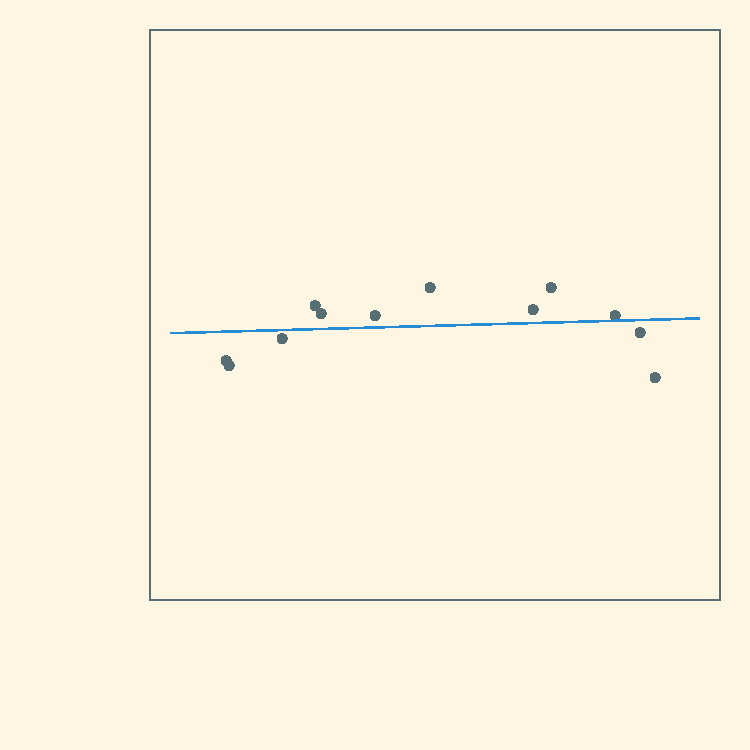
\includegraphics[width=\textwidth]{fig/train_linear}
    %     \caption{Linear Fit}
    % \end{subfigure}%
    % ~
    % \begin{subfigure}[t]{0.33\textwidth}
    %     \centering
    %     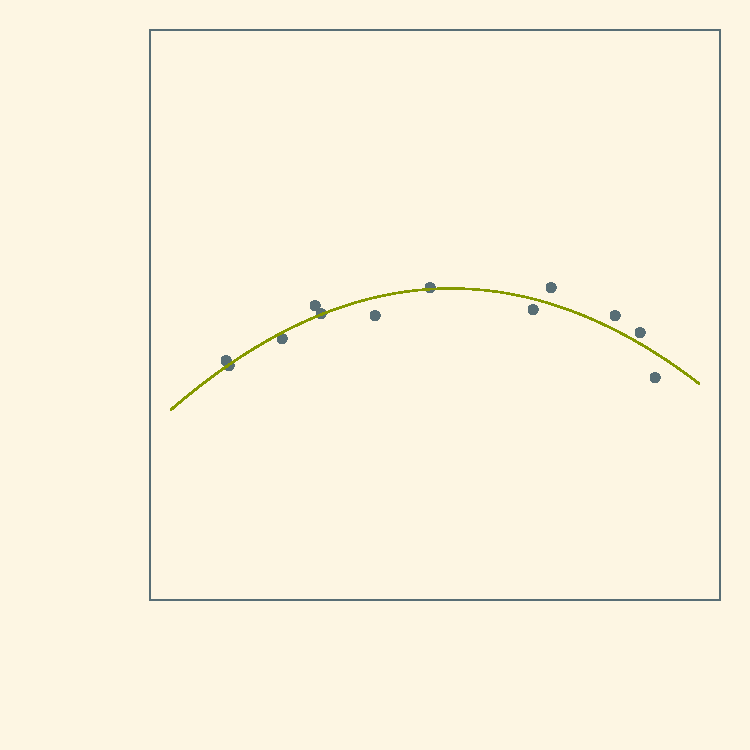
\includegraphics[width=\textwidth]{fig/train_quadratic}
    %     \caption{Quadratic Fit}
    % \end{subfigure}%
    % ~
    % \begin{subfigure}[t]{0.33\textwidth}
    %     \centering
    %     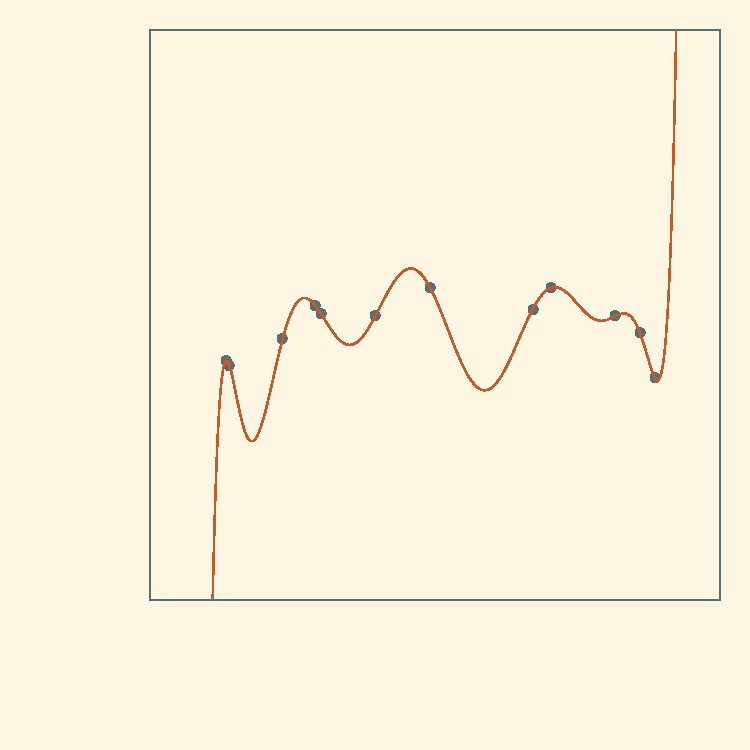
\includegraphics[width=\textwidth]{fig/train_overfit}
    %     \caption{Tenth-Order Fit}
    % \end{subfigure}
    \begin{subfigure}[t]{0.33\textwidth}
        \centering
        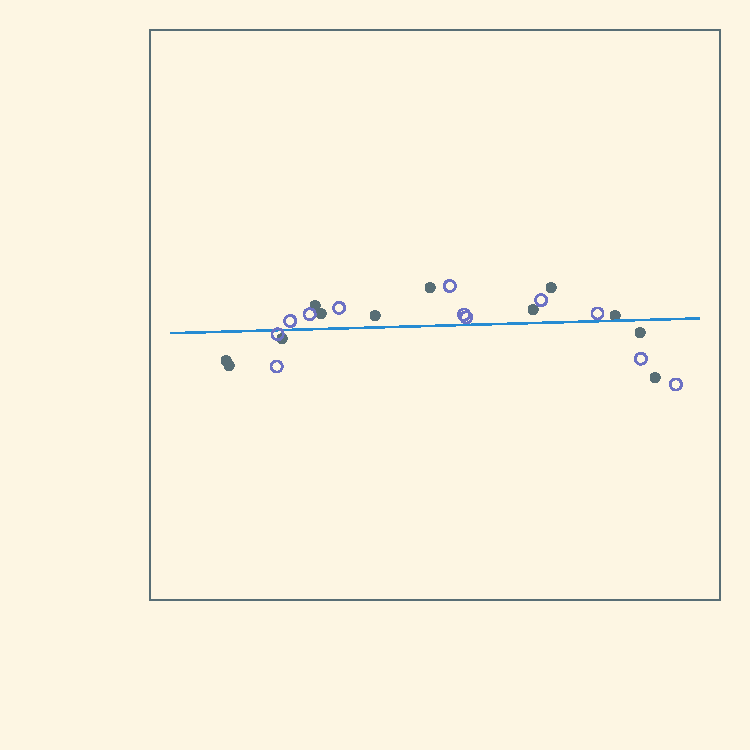
\includegraphics[width=\textwidth]{fig/test_linear}
        \caption{Linear Fit \label{fig:poly-linear}}
    \end{subfigure}%
    ~
    \begin{subfigure}[t]{0.33\textwidth}
        \centering
        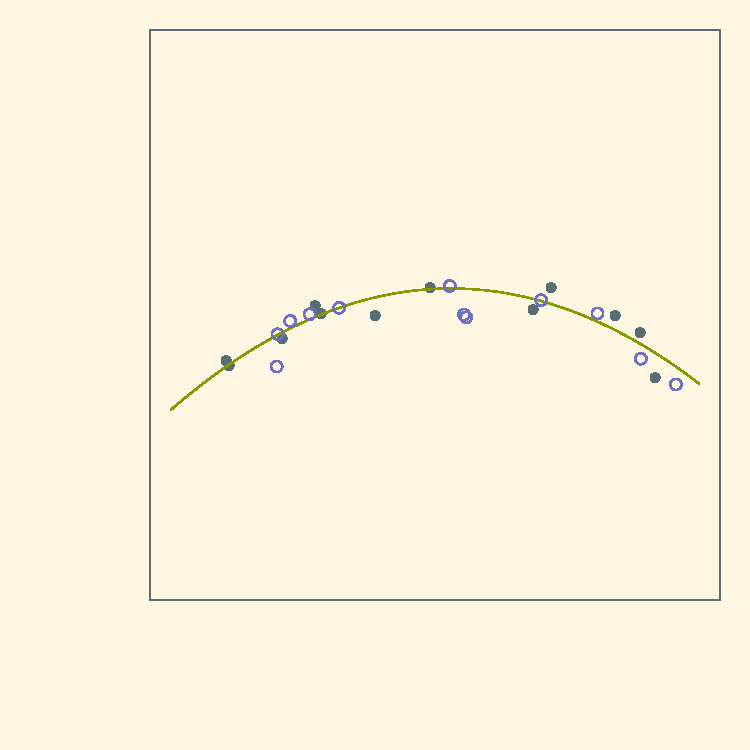
\includegraphics[width=\textwidth]{fig/test_quadratic}
        \caption{Quadratic Fit \label{fig:poly-quad}}
    \end{subfigure}%
    ~
    \begin{subfigure}[t]{0.33\textwidth}
        \centering
        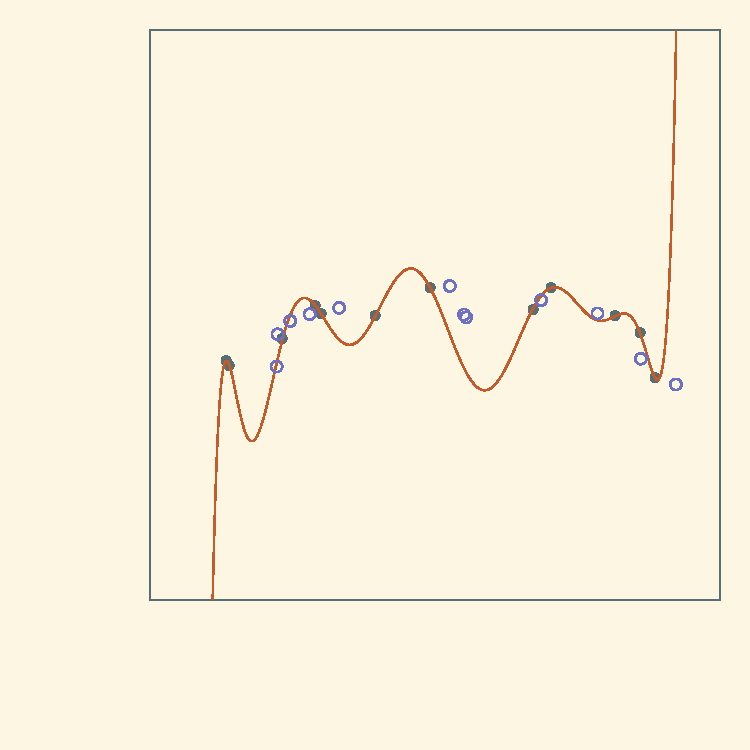
\includegraphics[width=\textwidth]{fig/test_overfit}
        \caption{Tenth-Order Fit \label{fig:poly10}}
    \end{subfigure}
    \begin{subfigure}[t]{0.5\textwidth}
        \centering
        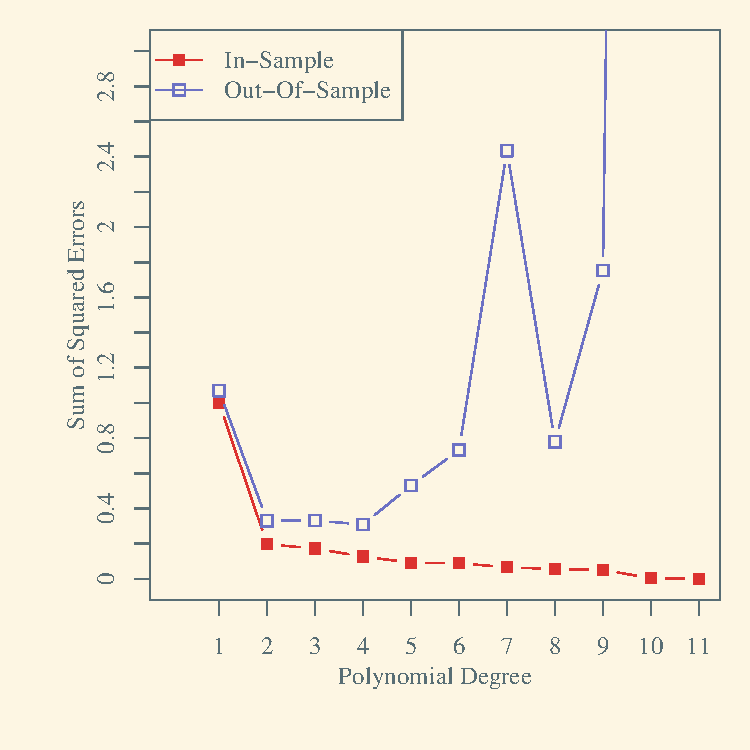
\includegraphics[width=\textwidth]{fig/poly_errors}
        \caption{Errors on Training and Test Set \label{fig:poly-errors}}
    \end{subfigure}
    \caption{\label{fig:polynomials} Polynomials of varying degrees fit using ordinary least
      squares (equivalently, maximum likelihood estimation) 
      to a set of eleven points generated from a fifth order
      polynomial with independent Normal
      residuals. \ref{fig:poly-linear}--\ref{fig:poly10}: fits of
      polynomial order 1, 2 and 10.  Filled circles are training data,
    unfilled circles are data not used during fitting.
    \ref{fig:poly-errors} squared prediction error in and out of the
    training sample for polynomial orders 1 through 10.}
\end{figure*}

\subsection{Balancing Fit and Complexity: Bayesian Occam's Razor}
\label{sec:balanc-fit-compl}

How do we go about deciding how complex a model to use in a given
setting?  One common approach is to use a penalized fit statistic, in
which the specific model $f$ is chosen not to maximize raw fit to the
data (e.g., by maximizing the likelihood), in which case more complex
models that contain simpler models as special cases will always be
chosen, but instead to maximize a {\em penalized} objective function
that balances in-sample fit with some measure of complexity.  This
complexity penalty can be viewed as a means to hold down the variance
of the model class; i.e., to combat overfitting.

Some examples of penalized fit measures that serve to select a subset
of predictor variables to receive nonzero coefficients in linear
regression are the lasso ($L_1$-penalized regression), Mallow's $C_p$,
and various ``information criteria'' such as AIC and BIC (TODO: ADD
CITATIONS).

Bayesian inference provides an alternative approach.  Whereas the
likelihood function serves as a measure of how surprising the data is given a fully
specified model, Bayesian inference provides a method for quantifying
how surprising the data and the specific model are together, where the
data is assumed to be selected stochastically from a set of possible
datasets allowed by the model (as in maximum likelihood estimation),
and additionally, the {\em model} is treated as though it were
selected stochastically from a set of possible models.  At each of
these choice points, if there are lots of options, any one of them
becomes more surprising.  

Consider the problem of choosing between two model
classes, $\mathcal{M}_1$ and $\mathcal{M}_2$, where $\mathcal{M}_1$
has no free parameters, and $\mathcal{M}_2$ has a free parameter
$\theta$, and reproduces $\mathcal{M}_1$ for a particular setting of
$\theta = \theta_*$.  The likelihood function by itself gives us no way by
itself to adjudicate between the two equivalent models,
$\mathcal{M}_1$ on the one hand, and $\mathcal{M}_2$ with $\theta =
\theta_*$ on the other since, $p(Y \given \mathcal{M}_1) = p(Y
\given \mathcal{M}_2, \theta_*)$.  Bayes' rule yields
\begin{align}
  p(\mathcal{M}_1 \given Y)&= \frac{p(\mathcal{M}_1) p(Y \given
    \mathcal{M}_1)}{p(Y)} \\
  p(\mathcal{M}_2 \given Y)&= \frac{p(\mathcal{M}_2) p(Y \given \mathcal{M}_2)}{p(Y)}
\end{align}
where in the case of $\mathcal{M}_2$, we need to expand the likelihood
to
\begin{equation}
  \label{eq:2}
  p(Y \given \mathcal{M}_2) = \int_{\Theta} p(Y \given \theta,
  \mathcal{M}_2) p(\theta \given \mathcal{M}_2) d\theta
\end{equation}
which is a weighted average of specific likelihoods of the form $p(Y
\given \theta, \mathcal{M}_2)$ with weights given by some distribution
over the parameter space.  Thus, if $\mathcal{M}_1$ assigns a large
likelihood to the observed data, even if $\mathcal{M}_2$ can achieve
the same likelihood at $\theta_*$, the ``good value'' $\theta_*$ will
be diluted in the {\bf marginal likelihood}, $p(Y
\given \mathcal{M}_2)$.

Hence, unlike maximum likelihood, 
Bayes theorem will tend to ``reward'' more restrictive {\em model
  classes} even in the case that the more flexible model contains the
simpler one as a special case, providing a built in Occam's Razor.
Of course, if there is some $\theta$ other than $\theta_*$ for which
the likelihood is greater, then $\mathcal{M}_2$ may win out depending
on whether the benefit to the likelihood outweighs the ``penalty''
induced by the $p(\theta \given \mathcal{M}_2)$ term, which is what we
want to happen, since the simplest model is only to be preferred if it
does about as good a job accounting for the data as the more complex model.

I now turn to the example of clustering a set of observations into
some number of groups, or, similarly, of fitting a mixture
distribution to a dataset.  I will introduce this problem in some
detail, since it is closely related to the main topic of this
dissertation, namely Hidden Markov Models, which I will introduce in
the following section, and treat in more detail in
Chapter \ref{chapter:HMM-NPBayes}.  I introduce the clustering
application here since it helps to motivate the bigger picture idea of
a nonparametric model.

\section{Clustering via a Mixture of Gaussians Model}
\label{sec:clustering}

Suppose we have a model of the form
\begin{equation}
  \label{eq:gmm}
  f(y \given \pi, \theta) = \sum_{k=1}^\infty \pi_k f(y \given \theta_k)
\end{equation}
where $\theta = (\theta_1, \theta_2, \dots)$ are some parameters
governing the mixture components, and $\pi = (\pi_1, \pi_2, \dots)$ is
the vector of mixing weights that sum to 1.

We could take a Bayesian approach and put priors on the vector of
mixture weights $\pi$ and on each
$\theta_k$.

Concretely, suppose that $f$ is Normal, so that $\theta_k = (\mu_k,
\sigma^2_k)$, and first suppose that we use a prior on $\pi_k$ that
fixes the number of nonzero weights to a finite value, $K$.  
Then the model is of the form
\begin{equation}
  f(y \given \pi, \theta) = \sum_{k=1}^K \pi_k \Norm{\mu_k}{\sigma^2_k}
\end{equation}

The $\pi_i$ define a categorical distribution over $K$ categories.
The categorical family has the conjugate prior
\begin{equation}
  f(\pi \given \xi) \propto \prod_{k=1}^K \pi_k^{\xi_k - 1}
\end{equation}
which is a {\bf Dirichlet distribution}.

We can also place conjugate priors on the $\mu_k$ and $\sigma_k$, such
as Normal and Inverse-Gamma, in the case of Normal components.

(Note that when $y$ is vector valued, $\mu$ becomes a mean vector and
$\sigma^2$ becomes a covariance matrix.  It is also possible to define
conjguate priors for these.)

Putting everything together and assuming Normal components, we have the joint prior:
\begin{equation}
  f(\pi, \mu, \sigma^{-2}) \propto \prod_{k=1}^K \pi_k^{\xi_k - 1}
  e^{-\frac{1}{2\sigma_k^2} (\mu_k
  - \mu_0)^2} \sigma_k^{-2a_0 - 2} e^{-\sigma_k^{-2} b_0}
\end{equation}
and the joint likelihood
\begin{equation}
  f(y \given \pi, \mu, \sigma^2) = \prod_{i=1}^n \sum_{k=1}^K \pi_k
  \sigma_k^{\frac{1}{2}} e^{-\frac{1}{2\sigma_k^2}(x_i - \mu_k)^2}
\end{equation}

That sum is trouble for inference.  
What we can do is to represent the likelihood in two stages: instead
of saying that each $y_i$ is drawn from a weighted mixture of the $K$
components, we can instead say that each $y_i$ comes from precisely
one component; we just do not know which one.  However, we can say
that $y_i$ comes from component $k$ with probability $k$.  We can
imagine generating data as follows:

For each $i = 1, \dots, n$
\begin{enumerate}
\item Draw $z_i \sim \mathrm{Categorical}(\pi_1, \dots, \pi_K)$
\item Draw $y_i \sim f(y \given \mu_{z_i}, \sigma^2_{z_i})$
\end{enumerate}

The joint likelihood for the $z_i$ and $y_i$ becomes
\begin{align}
  f(z_i, y_i \given \pi, \mu, \sigma^2) = f(z_i \given \pi) f(y_i
  \given z_i, \mu, \theta) &\propto \prod_{i=1}^n \pi_{z_i}
  (\sigma^2_{z_i})^{-1/2} e^{-\frac{1}{2\sigma^2} (y_i - \mu_{z_i})^2}\\
  &= \prod_{k=1}^K \pi_k^{n_k} (\sigma_k^2)^{-\frac{n_k}{2}}
  e^{-\frac{1}{2\sigma^2_k} \sum_{i: z_i = k} (y_i - \mu_k)^2}
\end{align}
which yields a posterior distribution with simple conditional
distributions that can be sampled from very straightforwardly using a
Gibbs sampler, in which the set of posterior variables is divided into
blocks, each of which is iteratively sampled from its conditional
posterior given the previous state of the others, which defines a
Markov Chain whose stationary distribution is the full posterior 
\citep{geman1984stochastic}.

\section{Clustering Sequential Data: The Hidden Markov Model}

In many applications, data are not i.i.d., but have some known
dependence structure.  Sequential data is one such case.  Suppose a
dataset consists of an ordered sequence of observations, ${y_t}, t =
1, \dots, T$.  Since unlike in the i.i.d. case we assume the order is
meaningful (most typically, the index $t$ might represent the time at which the data
point was collected), it is reasonable to expect that observing the
value at time $t$ would alter the predictive distribution at time
$t+1$, even if we knew the marginal distribution.  For example, $y_t$
might be a word or a sentence of text in a document, a snippet of a
sound recording, physiological measurements collected over time.  In
all of these cases, we expect nearby observations either to be
similar, or to be made more predictable given the last few observations.

One option would be to encode the dependencies among the data points
through a conditional model of the data at time $t$ given various
combinations of data at time $t-1$, $t-2$, \dots, $t-s$; that is, to
model the data using an order $s$ Markov chain. However, modeling the
distribution conditioned directly on observations risks an overly
complex conditioning structure, since in most settings there is likely
to be some idiosyncratic noise present in each observation that does
not depend on time in the same way as the underlying signal.  That is,
quite often the distribution at $t$ is likely to be a mixture of a temporally dependent
component and a temporally independent component.

The {\bf Hidden Markov Model}, first developed by
\citet{baum1966statistical} (see also \citet{rabiner1986introduction}
for a classic tutorial) separates temporal dynamics of an evolving
underlying (``hidden'') state from an temporally independent ``noise''
component by augmenting the observed time sequence $\{y_t\}, t = 1,
\dots, T$ with a latent data sequence, $\{z_t\}, t = 1,
\dots T$, such that at the distribution of the observations, $y_t$ are
independent conditioned on the latent sequence, $z_t$, but the $z_t$
evolve according to a Markov chain.  More formally, the model is
\begin{align}
  z_1 &\sim \Cat{\pi_{01}, \dots, \pi_{0J}} \\
  z_t \given z_{t-1} &\sim \Cat{\pi_{z_{t-1}1}, \dots,
    \pi_{z_{t-1}J}}, \quad t = 2, \dots, T
  \\
  y_t \given z_t &\sim F(\theta_{z_t}), \quad t = 1, \dots, T
\end{align}

where the vector $\pi_0 = (\pi_{01}, \dots, \pi_{0K})$ is the initial
distribution of the underlying Markov chain, the matrix $(\pi_{jj'}),
j,j' = 1, \dots, J$ is the transition matrix of the Markov chain, $F$
is a family of {\bf emission distributions}, which is parameterized
for each state in the Markov chain by the $\theta_j, j = 1, \dots, J$.

This model is nearly identical to the mixture model discussed in
Sec. \ref{sec:clustering}, the only difference being the dependence of
the label, $z_t$ on the previous label, $z_{t-1}$.  We can indeed
construct an easy to work with Bayesian HMM by placing an appropriate 
conjugate prior on the $\theta_t$ emission parameters (e.g.,
Normal-Inverse Wishart in the case where $F$ is the family of Normal
distributions), and a Dirichlet conjugate prior on $\pi_0$ and 
each row of $\pi$, and carry out posterior inference using Gibbs
sampling: alternating between sampling the state sequence $\{z_t\}$
and the model parameters, $\pi, \pi_0$ and the $\theta_j$.  There is
some additional difficulty introduced by the fact that the $z_t$
indicators are no longer conditionally independent, and so we must
either sample them jointly, or break up the Gibbs sampler into
many additional blocks so as to sample each $z_t$ conditioned on all
the others.  I will defer details of inference in this model until
Chapter \ref{chapter:HMM-NPBayes}.


\section{Model Selection in HMMs and the Mixture of Gaussians Model}
\label{sec:model-select-mixt}

It is relatively rare that we would be in a situation where we wanted
to fit a mixture of Gaussians to a dataset and knew exactly how many
components there were in the mixture.  It is perhaps somewhat more
likely that we know in advance how many
states the hidden Markov chain in an HMM can visit, but there are
certainly settings where we cannot or would not wish to do this. 
What can we do if we cannot specify $K$ ahead of time?

One approach is to apply the logic outlined in
Sec. \ref{sec:balanc-fit-compl} and simply put a prior distribution on
$K$, and then calculate (or sample from) the posterior distribution
over $K$.  Then, although we can always achieve at least as large a
likelihood with a larger $K$ as with a smaller $K$ (either by setting
some mixture weights to zero, or by effectively combining multiple
components into one by creating mixture components with
identical means and variances), since models with larger $K$ have more flexibility, their
marginal likelihood will tend to be diluted by all of the ways they can fit
the data badly.

However, this requires doing inference separately for as many values
of $K$ as we want to consider, and for the larger values of $K$, this
inference can be computationally expensive.  It turns out that we can
achieve substantially the same thing more simply by employing a single
{\bf nonparametric} model with an {\em infinite} number of
components.  

\section{The Structure of This Dissertation}

In the next chapter, I turn to the distinction between parametric and
nonparametric models, develop some of the theory of {\bf Dirichlet Process Mixture
  Models}, which form the basis for the infinite-state Hidden Markov
Model, which I define after that, along with additional detail on
Gibbs sampling in these two models.

In Chapter \ref{chapter:HaMMLeT}, I introduce a new model, the Hidden
Markov Model with Local Transitions (HaMMLeT), which generalizes the
infinite state Hidden Markov Model to allow more specific prior
information on the state space to be incorporated.  Then, in Chapters
\ref{chapter:cocktail-party} through Chapter \ref{chapter:music}, I
define variations on the basic HaMMLeT model in order to test the
model on several kinds of data.  Finally in Chapter
\ref{chapter:discussion} I give some concluding thoughts and outline
plans for future work.



\chapter{ \MakeUppercase{Bayesian Nonparametric Models and the Infinite
  Hidden Markov Model} }
\label{chapter:HMM-NPBayes}
\section{Parametric Vs. Nonparametric Models}
\label{sec:param-vs.-nonp}

Models that can be identified using a finite set of values
(that is, parameters) are called {\bf parametric} models.  Their
complexity and expressivity is the same whether they are fit using 10
data points, $10^6$ data points, or $10^10$ data points.  Most
canonical statistical models are parametric: the parameters in a
regression model comprise the regression coefficients and the
parameters of the residual distribution.  The parameters of the
mixture of Gaussians model comprise vector, $\pi$, of $K$ mixing weights,
and the parameters of the individual component Normal distributions:
$\{\mu_k, \sigma^2_k\}, k = 1, \dots, K$.

In a parametric model, once the sample size is a few orders of
magnitude larger than the number of parameters, the gains made by
further increasing the sample size, which in a frequentist setting
comes in the form of narrower confidence sets, and in a Bayesian
setting comes in the form of reduced posterior variance, are typically
negligible: the errors in prediction due to inevitable model misspecification, and
practical concerns with generalizability to new data sets, overwhelm
the remaining decimal places of uncertainty.

The name {\bf nonparametric model} is something of a misnomer, in that
nonparametric models do not have {\em no} parameters (a model with no
parameters would by definition be unable to learn anything from data);
rather, they have a number of parameters which grows adaptively as the
sample size increases.

A common frequentist family of nonparametric models are kernel-smoothed density
estimators \citep{rosenblatt1956remarks, parzen1962estimation}, 
in which the probability density of a data-generating process is
estimated by taking the empirical distribution and ``smoothing'' it to
obtain the estimated density at $y$ by
averaging together the values nearby points using a weight kernel.  As
a result, the estimated density requires $n$ values to specify it,
where $n$ is the sample size.  As such, the complexity of the family
of distributions in the model space grows with the sample size, unlike
in a parametric model.  Here, the tradeoff between bias and variance
is controlled not by the complexity of the model space, but rather by
the choice of smoothing bandwith: how much of the density at each
point is ``borrowed'' from nearby locations, with one extreme
representing a bandwidth of zero, in which case the estimate is simply
the empirical distribution.

It is natural to interpret the kernel density estimator as a mixture
model, where there is a mixture component centered at each data point
whose distribution belongs to a family defined by the kernel function:
for example, the Gaussian kernel results in a mixture of Gaussians,
the Epanechnikov kernel \citep{epanechnikov1969non} 
results in a mixture of Epanechnikov distributions, and the Uniform
kernel results in a mixture of Uniform distributions.  On the
interpretation that each component in a mixture model represents a
qualitatively distinct class of data, this means that each point is
viewed as qualitatively distinct, which from a Bayesian perspective
is unsatisfying.  Instead, we would like a model whose complexity
grows more slowly than linear in the sample size, such that as we
collect additional data it is always possible to encounter something
qualitatively new, but where the chances of doing so diminish as we
have more and more data.  This can be accomplished by employing a {\bf
Dirichlet Process} as the prior on the set of mixture components.

\section{The Dirichlet Process}
\label{sec:dirichlet-process}

The Dirichlet Process (DP) was formally defined by
\citet{ferguson1973bayesian} as a random probability measure, $G$, over a
$\mathcal{X}$ equipped with the sigma-algebra $\mathcal{A}$, with the
defining property that, for any partition of $\mathcal{X}$ consisting
of measureable sets, $A_1, A_2 \dots, A_k$, the random distribution given
by the probabilities
\begin{equation*}
  \{P(A_1), P(A_2), \dots, P(A_k)\}
\end{equation*}
has a Dirichlet distribution.

A Dirichlet distribution is defined by a mean distribution, $\pi_1,
\pi_2, \dots, \pi_k; \sum_i \pi_i = 1$, and a concentration parameter,
$\alpha$, which acts as an inverse variance parameter: as $\alpha$
goes to infinity, draws from the Dirichlet distribution are
distributions close to the mean with increasingly high probability.

The Dirichlet Process is also defined by a mean distribution $G_0$, called a
{\bf base measure}, and a
concentration parameter $\alpha$, but since the DP induces a Dirichlet
distribution over {\em any} finite partition of $\mathcal{X}$, the
mean distribution must be defined on all measureable
sets in $\mathcal{A}$.  We will write
\begin{equation}
G \sim \DP{\alpha G_0}
\end{equation}
to indicate that the random measure $G$ is distributed according to a
Dirichlet Process with base measure $G_0$ and concentration parameter $\alpha$.
Then, concretely, we have
\begin{equation*}
    P(A_1), P(A_2), \dots, P(A_k) \sim \Dir{\alpha G_0(A_1), \dots,
      \alpha G_0(A_k)}
\end{equation*}
An important probability of the DP is that the resulting measure is
discrete almost surely, and hence it is a sensible choice as a prior
on mixture components.  An equally important property when it comes to
using a DP as a Bayesian prior is that it is a {\em conjugate prior}
to a discrete likelihood. That is, if $n$ observations, $Y_1, \dots,
Y_n$, are drawn from
some unkown discrete probability measure $G$, and the prior employed
for $G$ is a Dirichlet Process, then the posterior distribution on $G$
is also a DP, whose base measure is a weighted sum of the prior base
measure, $G_0$, and the empirical distribution, $\hat{F}_n$:
\begin{equation}
  \label{eq:4}
  G \given Y \sim \alpha G_0 + n \hat{F}_n
\end{equation}
and whose concentration parameter is simply $\alpha + n$.

\subsection{The Normalized Gamma Process representation of the DP}
\label{sec:norm-gamma-proc}

\citet{ferguson1973bayesian} also showed that the Dirichlet Process
arises by normalizing a {\bf Gamma Process}.    
A Gamma Process is a stochastic point process on $\mathbb{R}^{+} \times
  \Theta$ which is defined by a {\bf L\'evy intensity measure}:
  \begin{equation}
    \label{eq:8}
    \nu(d\pi, d\theta) = \alpha \pi^{-1} e^{-\pi} d\pi G_0(d\theta)
  \end{equation}

  A realization of a Gamma process is a collection of point masses
  $\{\pi_k, \theta_k\}$, where $\pi_k \in \mathbb{R}^{+}$ is the mass
  associated with the point at location $\theta_k \in \Theta$.  This
  collection can be used to define a measure, $\mu$, on $\Theta$,
  where
  \begin{equation}
    \label{eq:3}
    \mu(A) = \sum_{k: \theta_k \in A} \pi_k
  \end{equation}

  The number $n(A)$ of point masses in a region $A \subset \mathbb{R}^+ \times \Theta$ is
  distributed as
  \begin{equation}
    \label{eq:9}
    n(A) \sim \Pois{\int_A \nu(d\pi, d\theta)}
  \end{equation}

  The L\'evy intensity measure of the Gamma process satisfies
  conditions to guarantee that the sum of all of the $\pi_k$
  weights is finite with probability 1, and therefore the measure $G$
  defined by
  \begin{equation}
    \label{eq:1}
    G = \frac{\mu}{\sum_k \pi_k}
  \end{equation}
  is a valid probability measure.  \citet{ferguson1973bayesian} showed
  that this probability measure is a DP with base measure $G_0$ and
  concentration $\alpha$, where
  these are the measure and parameter used in defining the L\'evy intensity of the
  Gamma process.

  Although the formal definition of the DP is well-defined, and
  although the Normalized Gamma Process representation guarantees
  existence of the DP, neither of these is terribly useful in {\em
    constructing} a DP, which limits the usefulness of the DP in
  applied modeling.  Fortunately, a constructive definition of the DP
  was discovered by \citet{sethuraman1994constructive}, using what is
  known as a {\bf Stick-Breaking Process}.

  \subsection{The Stick-Breaking Process construction of the DP}
  \label{sec:stick-break-proc}

  As shown by \citet{sethuraman1994constructive}, we can generate a
  draw from a Dirichlet Process by iteratively sampling the $\pi_k$
  weights, and then placing a point mass with weight $\pi_k$ at a
  location in $\Theta$ independently drawn from $G_0$.  This process
  is called a {\bf Stick-Breaking Process}.  By using the following
  algorithm to select the stick weights, the resulting collection of
  point masses has a Dirichlet Process.

  Having drawn $k-1$ point masses $(\pi_1, theta_1), \dots, (\pi_{k-1}, \theta_{k-1})$,
  \begin{enumerate}
  \item \label{stick-step-1} Draw $\tilde{\pi}_{k} \sim \Beta{1}{\alpha}$.
  \item \label{stick-step-2} Set $\pi_k = \tilde{\pi}_k \prod_{k'=1}^{K-1}
    (1 - \pi_{k'})$.
  \item \label{stick-step-3} Draw $\theta_k \sim G_0$.
  \end{enumerate}
  where, when $k = 1$, the null product in step \ref{stick-step-2} is
  1.

  The choice of $G_0$ and $\alpha$ determine the resulting DP.

  When describing the stick-breaking part of this process by itself
  --- that is, the process that produces the weights, $\pi_1, \pi_2,
  \dots$, it is common to write
  \begin{equation}
    \label{eq:11}
    \pi \sim \GEM{\alpha}
  \end{equation}
  where GEM stands for Griffiths-Engen-McCloskey, the names of three
  authors who did early work on stick-breaking processes and laid the foundation
  for the connection to Dirichlet Processes later formalized by
  \citet{sethuraman1994constructive}.
  
  \subsection{The Chinese Restaurant Process}
  \label{sec:chin-rest-proc}

  A useful construction for doing inference in a Dirichlet
  Process-based model is based on the metaphor of customers sharing
  food at a Chinese restaurant, which is normally described as
  follows.

  One by one, customers enter a Chinese restaurant and either sit at
  an unoccupied table and order a dish for the table, or join a table
  with other customers and share whatever dish is at the table.  The first
  customer necessarily starts a new table.  Subsequent customers join
  table $k$ with probability proportional to $n_k$, where $n_k$ is the
  number of customers currently seated at that table, and sit at an
  unoccupied table with probability proportional to a parameter
  $\alpha$.  

  More formally, the $n+1$th customer to enter the restaurant
  is assigned to table $k$ according to the distribution
  \begin{align}
    P(t_{n+1} = k) =
    \begin{cases}
      \frac{n_k}{n + \alpha} & k = 1, \dots, K \\
      \frac{\alpha}{n + \alpha} & k = K + 1
    \end{cases}
  \end{align}
  For each new table, a dish, $\theta_k$ is sampled from a base
  distribution, $G_0$.

  It turns out that the distribution of the collection of 
  assignments of dishes to customers is the same as the {\em marginal}
  distribution of draws from a random measure $G$ which is distributed
  $\DP{\alpha G_0}$ (see \citet{teh2011dirichlet} for a proof of this
  fact as well as a review of the theory of DPs in general).

  Notice that the Chinese Restaurant Process (CRP) has the property
  that the more often a dish has already been selected, the more
  likely it is to be selected again: that is, it has a ``rich get
  richer'' quality.  This makes sense in terms of the marginal
  distribution of draws from a DP-distributed random measure since,
  the more observations there are at a particular location, the
  stronger the evidence that the mass under $G$ at that location is
  large, and hence, the larger the posterior predictive probability at
  that location (marginalizing over $G$).

  \subsection{The Dirichlet Process Mixture Model}

  We are now ready to define a nonparametric version of a Bayesian
  Gaussian Mixture Model which replaces the Dirichlet distribution
  prior on the collection of mixture components from the fixed $K$ mixture model 
  with a Dirichlet Process prior.

  Reiterating the model initially defined in \eqref{eq:gmm}, suppose
  we have a model of the form
  \begin{equation}
    \label{eq:gmm-2}
    f(y \given \pi, \theta) = \sum_{k=1}^\infty \pi_k f(y \given \theta_k)
  \end{equation}
  where $\theta = (\theta_1, \theta_2, \dots)$ are some parameters
  governing the mixture components, and $\pi = (\pi_1, \pi_2, \dots)$ is
  the vector of mixing weights that sum to 1.  We now drop the
  assumption that all but finitely many of the $\pi_k$ are zero, and
  instead adopt as a prior:
  \begin{align}
    \label{eq:DP-prior}
    \{(\pi_k, \theta_k)_{k=1}^\infty\} \sim \DP{\alpha G_0}
  \end{align}
  As before, we introduce indicator variables, $\{z_i\}_{i=1}^n$ so
  that we can write
  \begin{align}
    \label{eq:5}
    P(z_i = k) = \pi_k, \qquad i = 1, \dots, n; k = 1, 2, \dots \\
    y_i \given z_i \sim F(\theta_{z_i})
  \end{align}
  where $F$ is a parametric family parameterized by $\theta$. For
  example, if $F$ is Normal, then $\theta$ might represent the mean
  vector and covariance matrix, and we might choose $G_0$ to be a
  Normal-Inverse Wishart distribution (or a non-conjugate choice as
  the application suggests).

  \subsection{Two Gibbs Samplers for DP Mixture Models}
  \label{sec:gibbs-sampler-dp}

  Given data, $y = (y_1, \dots, y_n)$ modeled using the mixture
  model in \eqref{eq:gmm-2} with the prior in \eqref{eq:DP-prior}, 
  we want to be able to make inferences about the parameters, $(\pi_k,
  \theta_k)$.  As with all but the simplest models, the full posterior
  is not amenable to exact analysis, and so we must resort to
  approximation to compute quantities of interest.  There are two
  dominant approximation methods in Bayesian inference.  One is variational
  inference, in which the true posterior is replaced by a distribution
  which is more amenable to analysis and which is in some sense as
  close as possible to the true distribution (usually the objective is
  to minimize the KL divergence from the target to the
  approximation).  The second popular approximation technique is
  Markov Chain Monte Carlo (MCMC), in which integrals involving the posterior
  are computed based on a sample from the posterior drawn using a
  Markov Chain whose transition kernel is chosen so as to yield the
  true posterior as the unique stationary distribution.  In a
  nutshell, variational Bayes provides an exact calculations based on an
  approximate distribution, whereas MCMC provides approximate
  calculations based on the true posterior.  I will focus on MCMC in
  this dissertation \citet{fox2012tutorial} for a tutorial on
  variational Bayes generally and \citet{blei2006variational} and
  \citet{kurihara2007collapsed} for work on variational methods for
  Dirichlet Process mixture models in particular.
  
  As with the finite mixture model, MCMC inference is greatly
  simplified by sampling over the $z_i$ indicators as well as over the
  mixture component parameters themselves (indeed, in some
  applications, these indicators may be the variables of primary
  interest).

  % The standard Gibbs sampling algorithm proceeds as follows
  % \begin{algorithm}
  %   \caption{Gibbs sampler for a Generic DP Mixture Model}
  %   \begin{algorithmic}[1]
  %     \State{Initialize the state labels, $z_1, \dots, z_n$ (e.g. from a
  %       a CRP)}
  %     \State{Define $K = \max_{i}\{z_i\}$}
  %     \For{Iteration $m = 1, \dots, M$}
  %         \For{$k = 1, \dots, K$}
  %         \State{Sample $\theta_k \given \{y_i: z_i = k\}$}
  %         \EndFor
  %     \EndFor
  %   \end{algorithmic}
  % \end{algorithm}
  
  We are interested in the joint posterior over the emission parameters,
  $\{\theta_k\}$, the component weights, $\{\pi_k\}$, and the component
  indicators, $\{z_i\}$, where $k$ indexes components and $i$ indexes
  observations.

  \paragraph{Method 1: A Collapsed Sampler Based on the CRP}
  One option is to sample only $\theta$ and $z$, integrating out
  $\pi$.  This is possible since the marginal distribution of $z
  \given \theta$ is a Chinese Restaurant Process.

  In this approach, we sample each entry of $z$ one at a time conditioned on the
  others.  Let $z^{(-i)}$ be the vector of component indicators
  excluding $z_i$, let $n_k^{(-i)} = \sum_{i' \neq i} \mathbb{I}(z_i = k)$ be the count
  of the number of $z_{i'}$ currently assigned to component $k$, not
  counting $z_i$, and let $K$ count the number of distinct values in
  $z$ among the other $n-1$ indicators (we will assume by permuting
  the labels that the distinct values are numbered $1$ through $K$).  Then we have
  \begin{align}
    p(z_i  = k \given z^{(-i)}) =
    \begin{cases}
      \frac{n_k}{n + \alpha}& \quad k = 1, \dots, K \\
      \frac{\alpha}{n + \alpha} & \quad k = K + 1
    \end{cases}
  \end{align}
  where if $z_i$ takes on a distinct value from any of the other
  entries in $z$, we call this value $K + 1$.

  In order to sample $z_i$ conditioned on both $z^{(-i)}$ and the
  data, we also need to compute the likelihood $p(y_i \given z_i, \theta)$ for
  each value of $z_i$.  Generically, we simply have
  \begin{align}
    p(y_i \given z_i, \theta) = f(y_i \given \theta_{z_i})
  \end{align}
  where $f(\cdot \given \theta_{z_i})$ is the density (or mass)
  function corresponding to the distribution $F(\theta_{z_i})$.

  Thus we sample $z_i$ with probabilities
  \begin{align}
    p(z_i  = k \given z^{(-i)}, y_i, \theta) \propto
    \begin{cases}
      \frac{n_k}{n + \alpha} f(y_i \given \theta_k) & \quad k = 1,
      \dots, K \\
      \frac{\alpha}{n + \alpha} \int_{\Theta} f(y_i \given \theta_*)
      p(\theta_*)\ d\theta_* & \qquad k = K+1
    \end{cases}
  \end{align}
  where depending on the form of $f$, it may be able to compute the
  integral for the marginal likelihood of $y_i$ analytically; but if
  not, we can approximate it by sampling a value of $\theta_*$ from
  the prior and using
  \begin{equation}
    \label{eq:1}
    p(z_i = K + 1 \given \theta, y) \propto \frac{\alpha}{n + \alpha} f(y_i \given theta_*)
  \end{equation}
  If $z_i$ is set to $K + 1$, we increment $K$.  If $z_i$ was
  previously the only indicator assigned to some value $k$, relabel
  the indicators to occupy consecutive natural numbers.

  Conditioned on $z$, sampling $\theta$ amounts to $K$ independent
  updates of the parameters of the $K$ separate components, each using
  the likelihood of the observations currently assigned to that
  component.  If the prior on $\theta$ is conjugate to the likelihood,
  this involves $K$ samples from an exponential family.

  \paragraph{Method 2: An uncollapsed sampler based on the
    Stick-Breaking Process}

  Alternatively we might choose to sample a finite subset of the
  entries in $\pi$ directly.  

  Conditioned on a current set of
  assignments to the $z$ indicators, we again let $K$ represent the
  number of distinct values taken on by the $z$, again assuming that
  the labels have been re-numbered as needed to take the values $1$
  through $K$, and again let $n_k, k = 1, \dots, K$ be the counts of
  the $z_i$ assigned to each $k$.  
  We can then sample the weights associated with each currently
  represented component, given by $\pi_1, \dots, \pi_K$, as well as
  the total weight associated with all unrepresented components
  combined, $\pi_{new}$.  Given the $n_k$, we have
  \begin{equation}
    \label{eq:2}
    (\pi_1, \dots, \pi_K, \pi_{new}) \sim \Dir{n_1, n_2, \dots, n_K, \alpha}
  \end{equation}
  We may then sample each $z_i$ according to
  \begin{align}
    p(z_i = k \given \pi, \theta, y) \propto
    \begin{cases}
      \pi_k f(y_i \given \theta_k) & \quad k = 1, \dots, K \\
      \pi_{new} \int_\Theta f(y_i \given \theta_*) p(\theta_*)\
      d\theta_* & k > K
    \end{cases}
  \end{align}
  where each time some $z_i$ is assigned to a new component, we must
  instantiate a new $\pi_{K+1}$ using the stick-breaking process, by sampling
  \begin{equation}
    \label{eq:6}
    \tilde{\pi}_{K+1} \sim \Beta{1}{\alpha},
  \end{equation}
  set $\pi_{K+1} := \pi_{new} \tilde{\pi}_{K+1}$, and set $\pi_{new}
  := 1 - \sum_{k=1}^{K+1} \pi_k$, and then increment $K$ before
  sampling the next $z_i$.

  Sampling $\theta$ is exactly as in the collapsed sampler, since
  the distribution depends only on $z$ and $y$.

\section{An Infinite State HMM}
\label{sec:an-infinite-state}

We would like to adapt the nonparametric DP mixture model to the
sequential setting to define an infinite state HMM 
in an analogous way to that in which the finite
mixture model was adapted to create a finite state HMM.  There, the
link between the mixture model and the $K$-state HMM was that the HMM
consisted of $K$ separate $K$-state mixture models: one associated
with each state.  That is, after visiting state $k$, the next
observation is drawn from mixture model $k$.

Naively, then, we might then try to define a countably infinite set of
mixture models, each with a DP prior, and after visiting component
$k$, draw the next observation from mixture model $k$.  However, if
the prior on the emission parameters $\theta$ is continuous, then with
probability 1 the set of mixture components will be non-overlapping,
and hence we will never revisit the same component twice.

% Perhaps instead we should draw only the mixing weights (that is, the
% transition probabilities) separately for
% each preceding state, and draw $\theta_j$ only once per
% column.  However, this will not do what we want either.  By drawing 
% probabilities from a Stick-Breaking
% Process we will tend to get probabilities that decrease as we go, and
% so by sampling the entries in each row of the transition matrix in
% order, we are introducing a bias for every state to transition toward
% states with low indices.  

\subsection{The Hierarchical Dirichlet Process}
\label{sec:hier-dirichl-proc}

The key property that we want in an Infinite State HMM needs to have
is that the mixture distributions need to be coupled --- that is, they
need to share a set of components.  In order to accomplish this using
a Dirichlet Process prior on the mixture parameters, the base measure
needs to be discrete.

\subsection{The HDP-HMM}
\label{sec:hdp-hmm}

\citet{teh2006hierarchical} defined the {\bf Hierarchical Dirichlet
  Process} (HDP), in which a collection of Dirichlet Processes take as
a common base measure a distribution itself drawn from a DP.  This
model is then hierarchical in the same sense as a Bayesian hierarchical regression
model, in which data sets from a collection of sources are assumed to
have similar distributions, and hence are given a common prior whose
parameters are informed by all of the data across sources.  

Formally, we define
\begin{align}
  G_0 \sim \DP{\gamma H}
\end{align}
and
\begin{align}
  G_j \sim \DP{\alpha G_0}, \quad j = 1, 2, \dots, J
\end{align}
where $\gamma$ is a concentration parameter that governs the
distribution of the weights of the atoms in the shared base measure
$G_0$, with larger $\gamma$ leading to probability mass being
dispersed among a large number of atoms, and smaller $\gamma$ leading
to a concentration of mass in just a few components.  The
concentration parameter $\alpha$ for the individual measures $G_j$
governs how tightly clustered the individual $G_j$ are around the mean
base measure $G_0$, with large $\alpha$ leading to the $G_j$ being
highly similar to $G_0$, and small $\alpha$ leading to each $G_j$
placing a lot of mass in a small number of components drawn from
$G_0$, such that the average across $G_j$s still looks like $G_0$, 
but where each $G_j$ may be quite different.

While the effect of $\gamma$ is clear enough from the Stick-Breaking
Process representation of DPs, it is worth examining how it is that
the second-level concentration $\alpha$ governs the behavior of the
atoms in the individual $G_j$.  We can see this using the
Stick-Breaking Process as well.

The effect of $\alpha$ is clearest when $\gamma$ is large, so that
$G_0$ has little bits of mass at lots of different places, with
location having much mass.  To draw a $G_j$ with this discrete $G_0$ 
as a base measure, we begin with a stick of unit mass, and break off a
mass by sampling from a
$\Beta{1}{\alpha}$ distribution.  We place a mass with this weight at
a random location drawn from the countable set of possibilities given
by $G_0$.  We then draw a random breaking point for remaining mass 
from another $\Beta{1}{\alpha}$ distribution, choose another location independently
from $G_0$, and so on.  First, imagine $\alpha$ is quite small.  Then
the first mass is likely to be quite near 1, the secon is likely to
take a large share of what's left, and so on.  So $G_j$ is likely to
place most of its mass at a few locations, though {\em which}
locations those are is uncertain due to the high dispersion in $G_0$.
At the other extreme, suppose $\alpha$ is quite large.  Then each time
we break off a mass, it is likely to be quite small, and it will take
many breaks and samples from $G_0$ before we accumulate significant
probability.  As a result, by the law of large numbers, 
the distribution of this large number of small masses is likely to
mimic closely the distribution in $G_0$.

TODO: add a figure illustrating combinations of alpha and gamma

\subsection{A Stick-Breaking Representation of the Aggregate Weights
  in an HDP}

The second-level Stick-Breaking Process describes the weights of the
atoms drawn from the base measure to form each $G_j$; however, since the base measure is
discrete, we will assign more than one stick to the same location;
thus if we want to describe the total mass that $G_j$ assigns to the
location $\theta_k$, we need to account for the fact that this mass is
the accumulation of infinitely many ``sticks''.  We can get a better
handle on the distribution of these masses by considering the defining
property of a Dirichlet Process random measure: namely, that the
distribution of the values of the measure over any finite partition of
$\Theta$ is a Dirichlet distribution.

Denote by $\theta_1, \theta_2, \dots$ the locations of the atoms in
$G_0$, with associated probabilities $\beta_1, \beta_2, \dots$.
Consider the finite partition $\{\{\theta_1\}, \Theta \setminus
\{\theta_1\}\}$, and define $\pi_{jk} := G_j(\theta_k), k = 1, 2,
\dots$.  Then,
\begin{align}
  (\pi_{j1}, 1 - \pi_{j1}) \sim \Dir{\alpha
    G_0(\theta_1), \alpha G_0(\Theta \setminus \theta_1)},
\end{align}
that is,
\begin{align}
  (\pi_{j1}, 1 - \pi_{j1}) \sim \Dir{\alpha
    \beta_1, \alpha (1 - \beta_1)},
\end{align}
Since the first component of a two-component Dirichlet distribution
has a Beta distribution with the same parameters, 
this means that $\pi_{j1} \sim \Beta{\alpha \beta_1}{\alpha(1 -
  \beta_1)}$.

More generally, for any $K$, we have
\begin{align}
  (\pi_{j1}, \dots, \pi_{jK}, \sum_{k=K+1}^{\infty} \pi_{jk}) \sim
  \Dir{\alpha \beta_1, \dots, \alpha \beta_K, \alpha
    \sum_{k=K+1}^{\infty} \beta_k}
\end{align}

Thus we can construct the $\pi_{jk}$ weights directly via the
following Stick-Breaking Process.  For $k = 1, 2, \dots$,
  \begin{enumerate}
  \item \label{stick-step-1} Draw $\tilde{\pi}_{jk} \sim \Beta{\alpha
      \beta_k}{\alpha (1 - \sum_{k'=1}^k \beta_{k'})}$.
  \item \label{stick-step-2} Set $\pi_{jk} = \tilde{\pi}_k \prod_{k'=1}^{K-1}
    (1 - \pi_{k'})$.
  \end{enumerate}

\subsection{A Normalized Gamma Process Representation of the Weights
  in the HDP}
\label{sec:norm-gamma-proc-1}

A Dirichlet distribution can be constructed by normalizing a set
of Gamma random variables, where the shape parameters are equal to the
parameters of the Dirichlet, and the rate parameters are a constant
(what constant does not matter, since it will be normalized out
anyway).  So we can write
\begin{align}
  \beta &\sim \GEM{\gamma} \\
  \tilde{\pi}_{jk} &\stackrel{ind}{\sim} \Gamm{\alpha \beta_k}{1} \\
  T_j &:= \sum_{k'} \tilde{\pi}_{jk'} \\
  \pi_{jk} &:= T_j^{-1} \tilde{\pi}_{jk}
\end{align}

Since the sum of independent Gamma variates with a common rate
parameter is a Gamma variate with the shared rate and whose shape is
the sum of the shapes, we have $T_j \sim \Gamm{\alpha}{1}$, and
conditioned on $T_j$ the $\pi_{jk}$ are independent.

\subsection{Adapting the HDP for an Infinite State HMM}

We could use the HDP to define a coupled collection of mixture models,
to model clustered data in several known contexts, as
\citet{teh2006hierarchical} did to define coupled infinite mixtures of
topics in various documents.  We can also use it to define a infinite
collection of infinite mixtures in the form of an HMM with infinitely
many states.  \citet{beal2001infinite} first described an infinite HMM
without explicitly making the connection to a Hierarchical Dirichlet
Process; \citet{teh2006hierarchical} showed that, with a few
differences, the model developed by \citeauthor{beal2001infinite}
could be derived using an HDP.

In the HMM setting, the ``data sources'' indexed by $j$ in the notation in the
previous section correspond to different previous states in the hidden
Markov chain, $\theta_j$ represents the emission parameters
associated with state $j$ each hidden state, and $G_j$ represents the
transition distribution from state $j$ to all other states (which are
identified by their respective $\theta_{j'}$, and due to discreteness
of $G_0$n, are the same countably infinite set for each source
state).  We will denote by $\pi_{jj'}$ the transition probability from
state $j$ to state $j'$, where we have replaced the $k$ subscript by
$j'$ to emphasize the fact that the set of source states and the set
of destination states are the same.

Then we can define the following prior on the elements of the transition matrix of the
HDP-HMM:
\begin{align}
  \beta &\sim \GEM{\gamma} \\
  \tilde{\pi}_{jj'} &\sim \Gamm{\alpha \beta_{j'}}{1} \\
  T_j &:= \sum_{j'} \tilde{\pi}_{jj'} \\
  \pi_{jj'} &:= T_j^{-1} \tilde{\pi}_{jj'} 
\end{align}
To complete the model, define a Markov chain over state indicators,
$\{z_t\}_{t=1}^T$, with infinite transition matrix $\pi =
(\pi_{jj'})$, a prior measure, $H$, on the collection of emission parameters
$\{\theta_j\}_{j=1}^\infty$, and the likelihood $F$:
\begin{align}
  z_t \given z_{t-1} &\sim \Discrete{\pi_{z_{t-1}1},\pi_{z_{t-1}2},
    \dots} \\
  \theta_j &\stackrel{i.i.d.}{\sim} H \\
  y_t \given z_t &\sim F(\theta_j)
\end{align}

\section{Inference in Finite and Infinite State HMMs}
\label{sec:inference-hdp-hmm}

A variety of inference algorithms have been developed for both finite
state and infinite state Bayesian Hidden
Markov Models, including variational methods (see \cite{beal2003variational} for
a review of the finite-state case, and \cite{johnson2014stochastic}
for the infinite-state case), and particle filters 
\citep{fearnhead2003line, tripuraneni2015particle}, as well as a number
of different Gibbs-sampling algorithms \citep{teh2006hierarchical,
  vangael2008beam, fox2008hdp, johnson2013bayesian}.  
The key difference among the Gibbs samplers is
the treatment of the latent state sequence, $\{z_t\}$.  One
distinction is whether each $z_t$ is put in its own block and sampled conditioned on
all of the others (as in \citeauthor{teh2006hierarchical}), or whether
the full $z_t$ sequence is sampled at once, as in
\citeauthor{vangael2008beam}, \citeauthor{fox2008hdp} and
\citeauthor{johnson2013bayesian}.  I focus here on the latter case,
since the Gibbs sampler developed in Chapter \ref{chapter:HaMMLeT} for
the new HaMMLeT model is of this type.

\subsection{The Forward Backward Algorithm}
\label{sec:forw-backw-algor-1}

In a non-dynamic mixture model, the component labels are mutually
independent given the component parameters, and hence a Gibbs sampler
can trivially sample all of them simultaneously.  In the dynamic case,
however, the distribution of each state indicator depends on the
previous indicator, which depends on the previous one, etc.
Moreoever, as a result of this propagation of dependence, the data at
time $t$ is indirect evidence for the indicators not just at time $t$,
but at {\em all other} times as well.  As a result,
sampling the $\{z_t\}$ sequence jointly requires care to appropriately
account for all of these dependencies.  The total number of possible
sequences in a model with $J$ states and $T$ observations is $T^J$,
which is an unmanageable number to consider exhausitvely.  In this section I derive the
{\bf forward-backward algorithm} (CITATION) for a $J$ state HMM.
The forward-backward algorithm is an efficient dynamic-programming
technique for sampling the $\{z_t\}$ sequence given the transition
matrix, $\pi$, the emission parameters, $\theta$, and the data, 
$y_1, \dots, y_T$, which requires only $O(J^2 T)$ computation.

Because of the Markov assumption, the set $\{z_1, \dots,
z_{t-1}\}$ is conditionally independent of the set $\{z_{t+1}, \dots,
z_{T}\}$, as well as of the data $\{y_{t+1}, \dots, y_{T}\}$, given
the indicator $z_t$.  The forward-backward algorithm
takes advantage of this conditional independence property to
iteratively compute the marginal distribution of each $z_t$ 
given only the data from $y_1$ through $y_t$ (the ``forward step''), 
and then sample the $\{z_t\}$ sequence starting with $z_T$ and working
backward to $z_1$ (the backward step).

I describe the backward step first, since this will make clearer the
need for the forward step.

\paragraph{The Backward Step}
In the backward step, we iteratively sample $z_t$ given $z_{t+1}$, and
the model parameters and data.  As noted above, conditioned on
$z_{t+1}$, $z_{t}$ is conditionally independent of all ``future''
data: $y_{t+1}, \dots, y_T$.  Using this fact and Bayes' rule, we have
\begin{align}
  p(z_{t}  = j \given z_{t+1}, y) &\propto p(z_t  = j \given z_{t+1}, y_1,
  \dots, y_t) \\
  &\propto p(z_t = j \given y_1, \dots, y_t) p(z_{t+1} \given z_t = j) \\
  &= b_t(j) \pi_{jz_{t+1}}
\end{align}
where $b_t(j)$ is shorthand notation for the probability
$p(z_t = j \given y_1, \dots, y_t)$, and we have omitted dependence on
$\pi$ and $\theta$ for conciseness.  Hence if we can compute $b_t(j)$
for each $j = 1, \dots, J$ and each $t = 1, \dots, T$, then it is
straigtforward to sample the $z_t$ sequence backward from $T$ to 1.
The computation of $b_t$ is the purpose of the forward step.

\paragraph{The Forward Step}
\label{sec:forward-step}

The goal of the forward step is to compute at each $t$ the partial posterior
distribution $b_t$ as defined above.  We can accomplish this via an
iterative ``message passing'' scheme, beginning at $b_1$.

By definition of the HMM we have
\begin{align}
  p(z_1 = j \given y_1) &\propto p(z_t = j) p(y_1 \given z_t = j) \\
  &= \pi_{0j} f(y_1 \given \theta_{j})
\end{align}

Now, suppose we have computed $b_t$ for some $t$.  Then we can
calculate the next ``message'', $b_{t+1}$ as follows, using the conditional independence
properties of the HMM:
\begin{align}
  b_{t+1}(j') &= p(z_{t+1} = j' \given y_1, \dots, y_{t+1}) \\
  &\propto p(z_{t+1} = j', y_1, \dots,
  y_{t+1})\\
  &\propto p(z_{t+1} = j', y_1, \dots, y_{t}) p(y_{t+1} \given z_{t+1} = j') \\
  &= \sum_{j} p(z_{t} = j, z_{t+1} = j',  y_1, \dots,
  y_{t}) p(y_{t+1} \given z_{t+1} = j') \\
  &= \sum_{j} p(z_{t} = j, y_1, \dots, y_{t})
  p(z_{t+1}  = j' \given z_{t} = j) p(y_{t+1} \given z_{t+1} = j') \\
  &\propto \sum_{j} b_{t}(j) \pi_{jj'} f(y_{t+1} \given \theta_{j'})
\end{align}

Thus to sample the full sequence $\{z_t\}_{t=1}^T$ we first do a
forward pass to calculate $b_t(j)$ for each $t,j$, and then
iteratively sample each $z_t$ beginning from $z_T$ and working backward
to $z_1$.  At each $t$ we need to compute $J^2$ products and a sum
over $J$ terms, and this needs to occur for each $t = 1, \dots, T$, so
the overall computation required for the forward step is $O(TJ^2)$.
The backward step requires only $TJ$ multiplications, and so the full
forward-backward algorithm is $O(TJ^2)$.

\subsection{Gibbs Sampling in the HDP-HMM}

In a finite-state HMM we can construct a straightforward Gibbs
sampler, employing the forward-backward algorithm to
sample the state sequence, $\{z_{t}\}$, conditioned on the data and
model parameters, and then conditioned on the state sequence, we can
update the model parameters as in a non-dynamic mixture model: if
conjugate priors are used, this can be done exactly; otherwise a
proposal distribution can be chosen and the result accepted according
to the Metropolis-Hastings acceptance probability formula.

In the HDP-HMM, however, we have infinitely many states to consider,
and so we cannot directly apply the forward-backward algorithm to
sample the state sequence, since it requires evaluating the
probability of being in every state at every time.  Thus if we want to
construct a Gibbs sampler for the HDP-HMM, we have a few obvious
options.  One is to sample each $z_t$ separately conditioned on the
rest of the sequence, integrating out the transition matrix.  
This is the approach taken in the Chinese
Restaurant Franchise representation, which also integrates out the top
level weights, $\beta$, as well as in the related auxiliary
variable sampler, which instantiates $\beta$, both originally described 
in \citet{teh2006hierarchical} (see that paper for details).  
Alternatively, we can use a finite-state approximation, either by
adaptively terminating the stick-breaking process once a target
proportion, $(1 - \varepsilon)$, for some suitably small choice of
$\epsilon$, of the stick has been broken off (this is referred to as a
{\bf truncated approximation}), or by simply picking a fixed reasonably
large but finite $J$.  This last approach is pursued by
\cite{fox2008hdp} and \cite{johnson2013bayesian} in their
generalizations of the HDP-HMM: the Sticky HDP-HMM and the HDP Hidden
Semi-Markov Model (HDP-HSMM), respectively.

\section{Local Transitions}
\label{sec:local-transitions}

HDP models have been widely adopted in Bayesian statistics and
machine learning.  However, a limitation of the vanilla HDP
is that it offers no mechanism to model correlations between mixture
components across contexts.  % Given the top level weights, one
% construction of the second level weights is to sample a collection of
% Gamma weights, one for each combination of context and component,
% which are all mutually independent, and then normalize within contexts
% to obtain valid mixture distributions; and so the only correlations
% possible between components are the small negative correlations 
% induced by normalization.
This is limiting in many applications, where we expect certain 
components to occur or not occur together.  In the HMM setting, 
we might expect certain states to exhibit similar incoming and
outgoing transition probabilities; that is, for certain rows and columns of the transition
matrix to be correlated.  In particular, we might expect pairs of states that are
``similar'' in some way to transition frequently to each other.  The
HDP-HMM offers no mechanism to model this similarity structure.  

In Chapter \ref{chapter:HaMMLeT}, I define a new model, the Hierarchical Dirichlet
Process Hidden Markov Model with Local Transitions (HDP-HMM-LT, or
HaMMLet, for short), which allows for correlations between rows and columns of the
transition matrix by assigning each state a location in an abstract metric 
space and promoting transitions between states
that are near each other.  I present a Gibbs sampling scheme
for inference in this model which employs an auxiliary variable scheme
to produce simple conditional distributions.  Then, in Chapters
\ref{chapter:cocktail-party} through \ref{chapter:music} I define
concrete instantiations of this model for several kinds of data, and
report experimental results showing that the new model in some cases
achieves better inference performance than existing models.




\chapter{\MakeUppercase{HaMMLeT: An Infinite Hidden Markov Model with
    Local Transitions}}
\label{chapter:HaMMLeT}
In this chapter, I describe a generalization of the Hierarchical
Dirichlet Process Hidden Markov Model \citet{teh2006hierarchical}
discussed in Chapter \ref{chapter:HMM-NPBayes} which introduces a
notion of latent similarity between pairs of hidden states, such that
transitions are a priori more likely to occur between states that are
deemed ``similar''.  This is achieved by placing a similarity function on
the space of state parameters which returns for each pair of states a
value between 0 and 1, representing the degree to which they are
similar (in whatever sense is desired for the application at hand),
and scaling HDP-generated transition probabilities by the similarity
between states.  I will refer to this model as the Hierarchical
Dirichlet Process Hidden Markov Model with Local Transitions
(HDP-HMM-LT, or HaMMLeT).  Although this achieves the goal of
selectively increasing the probability of transitions between similar
states, inference is made more complicated since, unlike in the
``vanilla'' HDP-HMM, the posterior measure over transition
distributions is no longer a Dirichlet Process --- that is, the prior
is no longer conjugate to the state sequence likelihood.

I will present an alternative representation of this process that
facilitates inference with an auxiliary variable scheme with the
following interpretation: The discrete time chain is recast as a
continuous time Markov Process in which: (1) some jump attempts fail,
(2) the probability of success is proportional to the similarity
between the source and destination states, (3) only successful jumps
are observed, and (4) the time elapsed between jumps, as well as the
number of unsuccessful jump attempts, are latent variables that are
sampled during MCMC inference.  By introducing these auxiliary latent
variables, nearly all conditional distributions in the model are
members of an exponential family, admitting exact Gibbs sampling.  The
only exception is the set of similarities, which are defined in an
application-specific way, and require application-specific inference
methods.  I present results for a few different choices in the
experiments in Chs \ref{chapter:cocktail-party} through
\ref{chapter:music}.

The motivating domain for this model is natural language text, in
which sentences in a document are associated with a set of ``topics'',
the topic sets in successive sentences have a high degree of overlap,
even when they are not identical (so that neighboring topic vectors
are similar), and in which there may be a high degree of correlation
between topics, so that modeling the entry and disappearance of each
topic independently is undesirable.  The topic vectors are represented
using binary vectors, indicating which topics are ``active'' in the
sentence, and to constrain the dynamics governing latent state
transitions so that transitions between similar topic vectors are {\it
a priori} more likely, but where certain topics tend to occur
together.  The latter property makes an ordinary factorial HMM
undesireable.

In the remainder of this chapter, I first review the transition
dynamics in the ``vanilla'' HDP-HMM so that it is easier to see how
the proposed HDP-HMM-LT differs; I then define the generative process
of the HDP-HMM-LT; finally, I introduce the ``Markov Jump Process With
Failed Transitions'' augmented data representation, which gives rise
to a natural Gibbs sampler for the HDP-HMM-LT model.

\section{Transition Dynamics in the HDP-HMM}
\label{sec:transition-dynamics}

The conventional HDP-HMM \citep{teh2006hierarchical} is based on a
Hierarchical Dirichlet Process which is defined as follows:

Each of a countably infinite set of states, indexed by $j$, receives a
parameter vector $\theta_j \in \Theta$, according to base measure $H$.
A top-level weight distribution, $\beta$, is drawn from the
Griffith-Engels-McClosky (GEM) stick-breaking process with 
parameter $\gamma > 0$, so that state $j$
has overall weight $\beta_j$, and an emission distribution which is
parameterized by $\theta_j$.
\begin{align} \theta_j &\stackrel{i.i.d.}{\sim} H \\ \beta &\sim
\GEM{\gamma}
\end{align}

The actual transition distribution from state $j$, denoted by $\pi_j$
is then drawn from a Dirichlet Process with concentration parameter
$\alpha$ and base measure $\beta$:
\begin{equation}
  \label{eq:1} \pi_j \stackrel{i.i.d}{\sim} \DP{\alpha \beta} \qquad j
= 1, 2, \dots
\end{equation}

The hidden state sequence is then generated according to the $\pi_j$.
Let $z_t$ be the index of the chain's state at time $t$.  Then we have
\begin{equation}
  \label{eq:4} z_t \given z_{t-1}, \pi_{z_{t-1}} \sim \pi_{z_{t-1}}
\qquad t = 1, 2, \dots, T
\end{equation} where $T$ is the length of the data sequence.

Finally, the emission distribution for state $j$ is a function of
$\theta_j$, so that we have
\begin{equation}
  \label{eq:5} y_t \given z_{t}, \theta_{z_t} \sim F(\theta_{z_t})
\end{equation}

A shortcoming of this model is that the generative process does not
take into account the fact that the set of source states is the same
as the set of destination states: that is, that the distribution
$\pi_j$ has an element which corresponds to state $j$.  Put another
way, there is no special treatment of the diagonal of the transition
matrix, so that self-transitions are no more likely {\it a priori}
than transitions to any other state.

The Sticky HDP-HMM \citep{fox2008hdp} addresses this issue by adding
an extra mass of $\kappa$ at location $j$ to the base measure of the
DP that generates $\pi_j$.  That is, they replace \eqref{eq:1} with
\begin{equation}
  \label{eq:6} \pi_j \sim \DP{\alpha\beta + \kappa \delta_j}.
\end{equation} An alternative model is presented by
\cite{johnson2013bayesian}, wherein state duration distributions are
modeled separately, and ordinary self-transitions are ruled out.  In
both of these models, auxiliary latent variables are introduced to
simplify conditional posterior distributions and facilitate Gibbs
sampling.  However, while both of these models have the useful
property that self-transitions are treated as ``special'', they
contain no notion of similarity for pairs of states that are not
identical: in both cases, when $j \neq j'$, the prior probability of
transitioning from $j$ to $j'$ depends only on the top-level stick
weight associated with state $j'$, and not on the identity or
parameters of the previous state $j$.

\section{An HDP-HMM With Local Transitions}

The goal of the proposed model is to add to the transition model the
concept of a transition to a ``nearby'' state, where nearness of $j$
and $j'$ may be defined deterministically or stochastically in terms
of the emission parameters, $\theta_j$ and $\theta_{j'}$, or may be
based on a latent state geometry that is a priori independent of the
emission distribution.

In order to accomplish this, we first consider an alternative
construction of the transition distributions, based on the Normalized
Gamma Process representation of the Dirichlet Process
\citep{ferguson1973bayesian}.

\paragraph{Notational Conventions} In the definitions and derivations
that follow, I will adopt the convention that variables written with
no subscript, such as $\theta$, $\beta$, and $\pi$, represent the
collection of all corresponding subscripted values: for example,
$\theta$ is the vector $(\theta_1, \theta_2, \dots)$, and $\pi$ is the
matrix $(\pi_{jj'})$.  For variables that represent counts, I will use
a dot in the subscript to represent a sum over corresponding
individual counts; for example, $n_{j\cdot}$ is used to represent
$\sum_{j'} n_{jj'}$, and $n_{\cdot\cdot}$ means $\sum_{j}\sum_{j'}
n_{jj'}$.

\subsection{A Normalized Gamma Process representation of the HDP-HMM}
\label{sec:normalized-gamma}

Define a random measure, $\mu = \sum_{j=1}^{\infty} \pi_j
\delta_{\theta_j}$, where
\begin{align} \pi_j &\stackrel{ind}{\sim}
\Gamm{\omega_j}{1} \label{eq:17}\\ T &= \sum_{j=1}^{\infty}
\pi_j \label{eq:18}\\ \tilde{\pi}_j &= \frac{\pi_j}{T} \label{eq:16}\\
\theta_j &\stackrel{i.i.d}{\sim} H \label{eq:19}
\end{align} and subject to the constraint that $\sum_{j\geq 1}
\omega_j < \infty$, which ensures that $T < \infty$ almost surely,
since
\begin{equation*} T \sim \Gamm{\sum_j \omega_j}{1}.
\end{equation*} As shown by Paisley et al. (2011), for fixed
$\{\omega_j\}$ and $\{\theta_j\}$, $\mu$ is distributed as a Dirichlet
Process with base measure $\nu = \sum_{j=1}^{\infty} \omega_j
\delta_{\theta_j}$.  If we draw $\beta$ from the GEM stick-breaking process
and then draw a series $\{\mu_m\}_{m=1}^M$ of i.i.d. random measures
from the above process, setting $w = \alpha\beta$ for some $\alpha >
0$, then this defines a Hierarchical Dirichlet Process.  If, moreover,
there is one $\mu_m$ associated with every state $j$, then we obtain
the HDP-HMM.

We can thus write
\begin{align} \beta &\sim \GEM{\gamma} \label{eq:20} \\ \theta_j
&\stackrel{i.i.d.}{\sim} H \label{eq:21}\\ \pi_{jj'}
&\stackrel{ind}{\sim} \Gamm{\alpha \beta_{j'}}{1} \label{eq:22}\\ T_j
&= \sum_{j'=1}^{\infty} \pi_{jj'} \\ \tilde{\pi}_{jj'} &=
\frac{\pi_{jj'}}{T_j} \label{eq:23},
\end{align} where $\gamma$ and $\alpha$ are prior concentration
hyperparameters for the two DP levels,
\begin{align}
  \label{eq:50} p(z_t \given z_{t-1}, \pi) = \tilde{\pi}_{z_{t-1}z_t}
\end{align} and the observed data $\{y_t\}_{t\geq 1}$ is distributed
as
\begin{equation}
  \label{eq:24} y_t \given z_t \stackrel{ind}{\sim} F(\theta_{z_t})
\end{equation} for some family, $F$ of probability measures indexed by
values of $\theta$.

\subsection{Promoting ``Local'' Transitions}
\label{sec:prom-local-trans}

In the preceding formulation, the transition distributions
$\{\pi_{j}\}_{j=1}^\infty$ are independent conditioned on the
top-level weights, $\beta$.  Our goal is to relax this assumption, in
order to allow for the possibility that there may be correlations
between these distributions.  We achieve this by introducing a notion
of a geometry on the state space; that is, that some pairs of states
are ``near'' to each other, and will thus tend to have similar
transition probabilities associated with them.

We associate with each state a location, $\ell_j \in \mathcal{L}$, and
define a ``similarity function'', $\phi: \mathcal{L} \times
\mathcal{L} \to [0,1]$, which returns for any pair of locations a
measure of how ``close'' they are.  

In order to remain agnostic about the extent to which $\phi$ is based
on the emission parameters, I will use $\theta_j$ to represent the
emission parameters for state $j$, and assume that $\ell_j$ determines
$\theta_j$, but that $\phi$ may be based on any part of $\ell_j$,
which may include some, all, or none of the information contained in
$\theta_j$.

I will also use the shorthand $\phi_{jj'}$ to represent $\phi(\ell_j,
\ell_{j'})$, for the sake of readability; but the reader should keep
in mind that whenever $\phi$ appears in a conditional distribution, it
is a constant if and only if $\ell$ is being conditioned on.

We can generalize the generative process defined in
\eqref{eq:20}-\eqref{eq:23} as follows:
\begin{align} \beta &\sim \GEM{\gamma} \\ \ell_j
&\stackrel{i.i.d}{\sim} H \\ \pi_{jj'} \given \beta, \theta &\sim
\Gamm{\alpha \beta_{j'}}{\phi_{jj'}^{-1}} \\ T_j &=
\sum_{j'=1}^{\infty} \pi_{jj'} \\ \tilde{\pi}_{jj'} &=
\frac{\pi_{jj'}}{T_j} \\ y_t \given z_t \stackrel{ind}{\sim}
F(\theta_{z_t})
\end{align} where $H$ is now a measure on $\mathcal{L}$.  In this new
formuation, the expected value of $\pi_{jj'}$ is
$\alpha\beta_{j'}\phi_{jj'}$.  Since a similarity between one object
and another should not exceed the similarity between an object and
itself, we will assume that $\phi_{jj'} = 1$ if $j = j'$.  We will
also assume that the similarity function is symmetric, so that
$\phi_{jj'} = \phi_{j'j}$ for all $j,j'$.  As we will see, either or
both of these assumptions could be relaxed if desired in a particular
application, but derivations presented here will make both.

The above model is equivalent to simply drawing the $\pi_{jj'}$ as in
\eqref{eq:20} and scaling each one by $\phi_{jj'}$ prior to
normalization, since it is a general property of Gamma distributions
that, if $X \sim \Gamm{a}{b}$, then $cX \sim \Gamm{a}{b/c}$.

Unfortunately, this formulation complicates inference significantly,
compared to the ordinary HDP-HMM, as the introduction of non-constant
rate parameters to the prior on $\pi$ destroys the conjugacy between
$\pi$ and $z$, and worse, the conditional likelihood function for
$\pi$ contains a sum which renders all entries within a row mutually
dependent {\em a posteriori}.

\section{The HDP-HMM-LT as a continuous-time Markov Jump Process with
``failed'' jumps}
\label{sec:dist-based-filt}

We can gain stronger intuition, as well as simplify posterior
inference, by re-casting the HDP-HMM-LT described in the last section
as a continuous time Markov Jump Process where some of the attempts to
jump from one state to another fail, and where the failure probability
increases as a function of the ``distance'' between the states.

Let $\phi$ be defined as in the last section, and let $\beta$,
$\theta$ and $\pi$ be defined as in the Normalized Gamma Process
representation of the ordinary HDP-HMM.  Specifically,
\begin{align}
  \label{eq:beta} \beta &\sim \GEM{\gamma} \\ \ell_j
&\stackrel{i.i.d}{\sim} H \\ \pi_{jj'} \given \beta &\sim \Gamm{\alpha
\beta_{j'}}{1}
\end{align} Now suppose that when the process is in state $j$, jumps
to state $j'$ are made at rate $\pi_{jj'}$.  This defines a
continuous-time Markov Process where the off-diagonal elements of the
transition rate matrix are the off diagonal elements of the $\pi$
matrix.  In addition, self-jumps are allowed, and occur with rate
$\pi_{jj}$.

If we only observe the jumps and not the durations between jumps, this
is an ordinary Markov chain, whose transition matrix is obtained by
appropriately normalizing the rows of $\pi$.  If we do not observe the
jumps themselves, but instead an observation is generated once per
jump from a distribution that depends on the state being jumped to,
then we have an ordinary HMM.

We modify this process as follows.  Suppose that each jump attempt
from state $j$ to state $j'$ has a chance of failing, which is an
increasing function of the ``distance'' between the states.  In
particular, let the success probability be $\phi_{jj'}$ (recall that
we assumed above that $0 \leq \phi_{jj'} \leq 1$ for all $j,j'$).
Then, the rate of successful jumps from $j$ to $j'$ is
$\pi_{jj'}\phi_{jj'}$, and the corresponding rate of unsuccessful jump
attempts is $\pi_{jj'}(1-\phi_{jj'})$.  To see this, denote by
$N_{jj'}$ the total number of jump attempts to $j'$ in a unit interval
of time spent in state $j$.  Since we are assuming the process is
Markovian, the total number of attempts is $\Pois{\pi_{jj'}}$
distributed.  Conditioned on $N_{jj'}$, $n_{jj'}$ will be successful,
where
\begin{equation}
  \label{eq:51} n_{jj'} \given N_{jj'} \sim
\Binom{N_{jj'}}{\phi_{jj'}}
\end{equation} It is easy to show (and well known) that the marginal
distribution of $n_{jj'}$ is $\Pois{\pi_{jj'}\phi_{jj'}}$, and the
marginal distribution of $N_{jj'} - n_{jj'}$ is
$\Pois{\pi_{jj'}(1-\phi_{jj'})}$.  The rate of successful jumps from
state $j$ overall is then $T_j := \sum_{j'} \pi_{jj'} \phi_{jj'}$.

Let $t$ index jumps, so that $z_t$ indicates the $t$th state visited
by the process (counting self-jumps as marking a transition to a new
time step).  Given that the process is in state $j$ at discretized
time $t$ (that is, $z_{t} = j$), it is a standard property of Markov
Processes that the probability that the destination $z_{t+1}$ of the
first successful jump is independent of the time since the last jump,
and the probability that $z_{t+1} = j'$ is proportional to the rate,
$\pi_{jj'}\phi_{jj'}$.

Let $\tau_{t}$ indicate the time elapsed between the $t-1$th and and
$t$th successful jump (where we assume that the first observation
occurs when the first successful jump from a ``dummy'' initial state
is made).  We have
\begin{equation}
  \label{eq:52} \tau_t \given z_{t-1} \sim \Exp{T_{z_{t-1}}}
\end{equation} where $\tau_t$ is independent of $z_{t}$.

During this period, there will be some number of unsuccessful attempts
to jump to each state, where the rate of unsuccessful jump attempts
from to state $j'$ is given by $\pi_{z_{t-1}}(1 - \phi_{z_{t-1}j'})$.
Denote by $\tilde{q}_{j't}$ the number of unsuccessful jump attempts
to $j'$ during the interval with duration $\tau_t$.  Then we have
\begin{equation}
  \label{eq:53} \tilde{q}_{j't} \given z_{t-1}, \tau_t \sim
\Pois{\tau_t \pi_{z_{t-1}j'}(1-\phi_{z_{t-1}j'})}
\end{equation}

Define the following additional variables
\begin{align}
  \label{eq:56} \mathcal{T}_j &= \{t \given z_{t-1} = j\} \\ q_{jj'}
&= \sum_{t \in \mathcal{T}_j}\tilde{q}_{j't} \\ u_j &= \sum_{t \in
\mathcal{T}_j} \tau_t.
\end{align} In addition, let $Q = (q_{jj'})_{j,j' \geq 1}$ be the
matrix of unsuccessful jump attempt counts, and $u = (u_j)_{j \geq 1}$
be the vector whose $j$th entry is the total time spent in state $j$.

Since each of the $\tau_t$ with $t \in \mathcal{T}_j$ are
i.i.d. $\Exp{T_j}$, and since the sum of $n$ Exponential random
variables with shared scale $\lambda$ has a $\Gamm{n}{\lambda}$
distribution, we have
\begin{equation} u_j \given z, \pi, \ell \stackrel{ind}{\sim}
\Gamm{n_{j\cdot}}{T_j}
\end{equation} where we define $n_{j\cdot} = \sum_{j'} n_{jj'}$, where
$n_{jj'}$ is the number of successful jumps from state $j$ to $j'$ and
$n_{j\cdot}$ is the total number of times that state $j$ is visited.

Moreover, since the $\tilde{q}_{j't}$ with $t \in \mathcal{T}_j$ are
Poisson distributed, the total number of failed attempts in the total
duration $u_j$ is
\begin{equation}
  \label{eq:60} q_{jj'} \stackrel{ind}{\sim}
\Pois{u_j\pi_{jj'}(1-\phi_{jj'})}.
\end{equation}

Thus if we marginalize out the individual $\tau_t$ and
$\tilde{q}_{j't}$, we have a joint distribution over $z$, $u$, and
$Q$, conditioned on the transition rate matrix $\pi$ and the success
probability matrix $\phi$, which is
\begin{align}
  \label{eq:54} p(z, u, Q \given \pi, \ell) &= \left(\prod_{t=1}^T
p(z_{t} \given z_{t-1})\right) \prod_{j} p(u_j \given z, \pi, \ell)
\prod_{j'} p(q_{jj'} \given u_j \pi_{jj'}, \phi_{jj'}) \\ &=
\left(\prod_{t}
\frac{\pi_{z_{t-1}z_t}\phi_{z_{t-1}z_t}}{T_{z_{t-1}}}\right) \prod_{j}
\frac{T_j^{n_{j\cdot}}}{\Gamma(n_{j\cdot})} u_j^{n_{j\cdot} - 1}
e^{-T_j u_j} \\ &\qquad\qquad\times \prod_{j'}
e^{-u_j\pi_{jj'}(1-\phi_{jj'})} u_j^{q_{jj'}} \pi_{jj'}^{q_{jj'}}
(1-\phi_{jj'})^{q_{jj'}} (q_{jj'}!)^{-1} \\ &= \prod_{j}
\Gamma(n_{j\cdot})^{-1} u_j^{n_{j\cdot} + q_{j\cdot}-1} \\
&\qquad\qquad \times \prod_{j'} \pi_{jj'}^{n_{jj'} + q_{jj'}}
\phi_{jj'}^{n_{jj'}} (1-\phi_{jj'})^{q_{jj'}}
e^{-\pi_{jj'}\phi_{jj'}u_j} e^{-\pi_{jj'}(1-\phi_{jj'})u_j}
(q_{jj'}!)^{-1} \\ &\label{eq:joint-likelihood} = \prod_{j}
\Gamma(n_{j\cdot})^{-1} u_j^{n_{j\cdot} + q_{j\cdot}-1} \prod_{j'}
\pi_{jj'}^{n_{jj'} + q_{jj'}} \phi_{jj'}^{n_{jj'}}
(1-\phi_{jj'})^{q_{jj'}} e^{-\pi_{jj'}u_j} (q_{jj'}!)^{-1}
\end{align}

\subsection{An HDP-HSMM-LT modification}
\label{sec:an-hsmm-modification}

In any Hidden Markov Model, the distribution of the number of time
steps for which a given hidden state persists is by definition a
Geometric distribution, where the ``failure'' parameter is the
relevant entry on the diagonal of the transition matrix.  The HDP-HMM
and the HDP-HMM-LT as defined above are no exception.  Although the
Sticky HDP-HMM \cite{fox2008hdp} and the LT generalization presented
here provide mechanisms for which the diagonal entries of the
transition matrix will tend to have greater mass than the off-diagonal
entries, they do not alter the Markovian assumption, which implies
Geometric durations.

The HDP Hidden Semi-Markov Model (HDP-HSMM;
\citet{johnson2013bayesian}) gets around this restriction directly, by
treating self-transitions as fundamentally distinct from all other
transitions, and modeling state persistence durations directly.
Should it be desireable to combine this property with the general
similarity bias of the HDP-HMM-LT, it is trivial to modify the LT
model to incorporate a separate duration model.  We can simply fix the
diagonal elements of $\pi$ to be zero, and allow $D_t$ observations to
be emitted $i.i.d.$ $F(\theta_{z_t})$ at jump $t$, where
\begin{equation}
  \label{eq:95} D_t \given z \stackrel{ind}{\sim} g(\omega_{z_t})
\qquad \omega_j \stackrel{i.i.d}{\sim} G
\end{equation} The likelihood then includes the additional term for
the $D_t$, and the only inference step which is affected is that,
instead of sampling $z$ alone, we sample $z$ and the $D_t$ jointly, by
defining
\begin{equation} z^*_s = z_{\max\{T \given s \leq \sum_{t=1}^T D_t\}}
\end{equation} where $s$ ranges over the total number of observations,
and associating a $y_s$ observation sequence with each $z^*_s$.
Inferences about $\phi$ are not affected, since the diagonal elements
are assumed to be 1 anyway.

In the HDP-HSMM as it is presented in \cite{johnson2013bayesian},
zeroing out the diagonal of the transition matrix to isolate
self-transitions to the separate duration model necessitates
renormalization of the other entries so that the rows of the
transition matrix are probability distributions.  As a result, the
conditional posterior for the matrix is no longer in an exponential
family.  To deal with this, \citeauthor{johnson2013bayesian} introduce
auxiliary variables which can be interpreted as the diagonal entries
of the transition matrix prior to zeroing out, as well as the number
of self-transitions that would have occurred for each state had the
transition matrix diagonal governed self-transitions instead of the
separate duration model.  Conditioned on these auxiliary variables,
conjugacy between the transition matrix prior and likelihood is
restored, and Gibbs sampling is able to proceed with exponential
family updates.

In the LT model, on the other hand, we are already representing the
transition matrix in unnormalized form, having rendered the entries
conditionally independent given the $z$ state sequence and the $u$
holding times, so we are free to clamp the diagonal entries at zero
without introducing a need for additional auxiliary variables in order
to achieve semi-Markov dynamics.

\subsection{Choice of Similarity Function}
The similarity function, $\phi$
bears resemblance to a kernel function, as used in a number of machine
learning methods, for example, to project data into a new feature space in
for a Support Vector Machine, or as a covariance function for a
Gaussian Process.  Although the role of the similarity function here
is similar, the restrictions on the similarity function here are different
than the restrictions that define a valid kernel, which is why I have
avoided using the term ``kernel'' in this context.  For the HaMMLeT
model, the similarity function must satisfy three properties:
\begin{enumerate}
\item It is bounded above.
\item It is nonnegative.
\item It is not identically zero.
\end{enumerate}

Given the motivation for the model and the intuitive properties of a
``similarity'' function, it seems natural to assume
additionally that $\phi$ is symmetric, and that it attains its upper
bound when evaluating the similarity between a state and itself; that
is, that $\phi_{jj'} = \phi_{j'j} \leq \phi_{jj} = 1$ for all $j,j'$.
However, strictly speaking there is no technical requirement that this
be the case; as long as the three conditions above are satisfied, the
normalization constant in the Normalized Gamma Process representation 
will be finite and positive, and the Markov Process with Failed Jumps
interpretation will hold (possibly after a global rescaling and
absorbing the constant into the
normalization so that $\phi_{jj'} \leq 1$ for all $j,j'$).

Some natural choices of similarity function are the following, all of
which depend on a distance function, $d_\lambda$.
\begin{enumerate}
\item The Laplacian kernel: $\phi(x,y) = \exp(-d_{\lambda}(x,y))$
\item The Gaussian kernel: $\phi(x,y) = \exp(-d_{\lambda}(x,y)^2)$
\item \label{rational} Functions of the form:
  \begin{equation*}
  \phi(x,y) = \left(c +
    d_{\lambda}(x,y)^p\right)^{-q} \text{ for positive constants $c$,
  $p$ and $q$}
  \end{equation*}
\end{enumerate}
where \label{rational} encompasses traditional kernel functions
including the Cauchy, Generalized Student's $t$, rational quadratic,
and inverse multiquadratic as special cases.

Notably absent from this list are kernel functions that take negative
values, such as the linear, polynomial, log kernels, and wave kernels, among others.

\subsection{Summary}
\label{sec:model-summary}

I have defined the following augmented generative model for the
HDP-H(S)MM-LT:
\begin{align}
  \label{eq:96} \beta &\sim \GEM{\gamma} \\ \ell_j
&\stackrel{i.i.d}{\sim} H \\ \pi_{jj'} \given \beta &\sim \Gamm{\alpha
\beta_{j'}}{1} \\ z_{t} \given z_{t-1}, \pi, \ell &\sim \sum_{j}
\left(\frac{\pi_{z_{t-1}j}\phi_{z_{t-1}j}}{\sum_{j'}
\pi_{z_{t-1}j'}\phi_{z_{t-1}j'}}\right)\delta_j \\ u_j \given z, \pi,
\ell &\stackrel{ind}{\sim} \Gamm{n_{j\cdot}}{\sum_{j'}
\pi_{jj'}\phi_{jj'}} \\ q_{jj'} \given u, \pi, \ell
&\stackrel{ind}{\sim} \Pois{u_j(1 - \phi_{jj'})\pi_{jj'}} \\
  \label{eq:likelihood} y_t \given z, \ell &\sim F(\theta_{z_t})
\end{align}

If we are using the HSMM variant, then we simply fix $\pi_{jj}$ to 0
for each $j$, draw
\begin{align}
  \label{eq:97} \omega_j &\stackrel{i.i.d}{\sim} G \\ D_t \given z
&\stackrel{ind}{\sim} g(\omega_{z_t}),
\end{align} for chosen $G$ and $g$, set
\begin{equation}
  \label{eq:98} z^*_s = z_{\max\{T \given s \leq \sum_{t=1}^T D_t\}}
\end{equation} and replace \eqref{eq:likelihood} with
\begin{equation}
  \label{eq:likelihood-hsmm} \by_s \given z, \theta \sim
F(\theta_{z^*_s})
\end{equation}

\section{MCMC Inference in the ``Failed Jumps'' Representation}
\label{sec:inference}

I develop a Gibbs sampling algorithm based on the Markov Process with
Failed Jumps representation, augmenting the data with the duration
variables $u$, the failed jump attempt count matrix, $Q$, as well as
additional auxiliary variables which we will define below.  In this
representation the transition matrix is not modeled directly, but is a
function of the unscaled transition matrix $\pi$ and the similarity
matrix $\phi$.  The full set of variables is partitioned into three
blocks: (1) $\{\gamma, \alpha, \beta, \pi\}$, (2) $\{z, u, Q, \xi\}$,
and (3) $\{\ell\}$, where $\xi$ is a placeholder for an additional set
of auxiliary variables that will be introduced below.  The variables
in each block are sampled jointly conditioned on the other two blocks.
In some of the applications described in later chapters, blocks (2)
and (3) can be sampled jointly, and if desired, the parameters of the
$\phi$ function can be given priors and sampled as a separate block.

Since we are representing the transition matrix of the Markov chain
explicitly, we approximate the stick-breaking process that produces
$\beta$ using a finite Dirichlet distribution with a number of
components larger than we expect to need, forcing the remaining
components to have zero weight.

Let $J$ indicate the maximum number of states.  Then, we approximate
\eqref{eq:beta} with
\begin{equation}
  \label{eq:28} \beta \given \gamma \sim \mathrm{Dirichlet}(\gamma /
J, \dots, \gamma / J)
\end{equation} This distribution converges weakly to the
Stick-Breaking Process as $J \to \infty$ \cite{ishwaran2000markov}.
In practice, $J$ is large enough when the vast majority of the
probability mass in $\beta$ is allocated to a strict subset of
components, or when the latent state sequence $z$ never uses all $J$
available states, indicating that the data is well described by a
number of states less than $J$.

\subsection{Sampling $\pi$, $\beta$, $\alpha$ and $\gamma$}
\label{sec:sampling-pi}

The joint conditional over $\gamma$, $\alpha$, $\beta$ and $\pi$ given
$z$, $u$, $Q$, $\xi$ and $\theta$ will factor as
\begin{equation}
  \label{eq:46} p(\gamma, \alpha, \beta, \pi \given z, u, Q, \xi,
\theta) = p(\gamma \given \xi) p(\alpha \given \xi) p(\beta \given
\gamma, \xi) p(\pi \given \alpha, \beta, \theta, z)
\end{equation} I will derive these four factors in reverse order.

\paragraph{Sampling $\pi$}

The entries in $\pi$ are conditionally independent given $\alpha$ and
$\beta$, so we have the prior
\begin{equation}
  \label{eq:47} p(\pi \given \beta, \alpha) = \prod_{j} \prod_{j'}
\Gamma(\alpha\beta_{j'})^{-1} \pi_{jj'}^{\alpha\beta_{j'} - 1}
\exp(-\pi_{jj'}),
\end{equation} and the likelihood given augmented data $\{z, u, Q\}$
given by \eqref{eq:joint-likelihood}.  Combining these, we have
\begin{align}
  \label{eq:61} p(\pi, z, u, Q \given \beta, \alpha, \theta) &=
\prod_{j} u_j^{n_{j\cdot} + q_{j\cdot} - 1}\prod_{j'}
\Gamma(\alpha\beta_{j'})^{-1} \pi_{jj'}^{\alpha\beta_{j'} + n_{jj'} +
q_{jj'} - 1} \\&\qquad \times e^{-(1 + u_j) \pi_{jj'}}
\phi_{jj'}^{n_{jj'}} (1-\phi_{jj'})^{q_{jj'}} (q_{jj'}!)^{-1}
\end{align} Conditioning on everything except $\pi$, we get
\begin{align}
  \label{eq:24} p(\pi \given Q, u, z, \beta, \alpha, \theta) &\propto
\prod_j \prod_{j'} \pi_{jj'}^{\alpha\beta_{j'} + n_{jj'} + q_{jj'} -
1} \exp(-(1 + u_j)\pi_{jj'})
\end{align} and thus we see that the $\pi_{jj'}$ are conditionally
independent given $u$, $z$ and $Q$, and distributed according to
\begin{align}
  \label{eq:25} \pi_{jj'} \given n_{jj'}, q_{jj'}, \beta_{j'}, \alpha
\stackrel{ind}{\sim} \Gamm{\alpha\beta_{j'} + n_{jj'} + q_{jj'}}{1 +
u_j}
\end{align}


\paragraph{Sampling $\beta$}
\label{sec:sampling-bbeta}

Consider the conditional distribution of $\beta$ having integrated out
$\pi$.  The prior density of $\beta$ from \eqref{eq:28} is
\begin{equation}
  \label{eq:62} p(\beta \given \gamma) =
\frac{\Gamma(\gamma)}{\Gamma(\frac{\gamma}{J})^J} \prod_{j}
\beta_j^{\frac{\gamma}{J} - 1}
\end{equation} After integrating out $\pi$ in \eqref{eq:61}, we have
\begin{align} p(z, u, Q \given \beta, \alpha, \gamma, \theta) &=
\prod_{j=1}^J u_{j} ^{-1} \prod_{j'=1}^J u^{n_{jj'} + q_{jj'} - 1}(1 +
u_j)^{-(\alpha\beta_{j'} + n_{jj'} + q_{jj'})} \\ &\qquad \qquad
\times \frac{\Gamma(\alpha\beta_{j'} + n_{jj'} +
q_{jj'})}{\Gamma(\alpha\beta_{j'})}
\phi_{jj'}^{n_{jj'}}(1-\phi_{jj'})^{q_{jj'}} (q_{jj'}!)^{-1} \\ &=
\prod_{j=1}^J \Gamma(n_{j\cdot})^{-1} u_j^{-1}(1+u_j)^{-\alpha}
\left(\frac{u_j}{1+u_j}\right)^{n_{j\cdot} + q_{j\cdot}} \\ &\qquad
\qquad \times \prod_{j' = 1}^J \frac{\Gamma(\alpha\beta_{j'} + n_{jj'}
+ q_{jj'})}{\Gamma(\alpha\beta_{j'})}
\phi_{jj'}^{n_{jj'}}(1-\phi_{jj'})^{q_{jj'}} (q_{jj'}!)^{-1}
\end{align} where we have used the fact that the $\beta_j$ sum to 1.
Therefore
\begin{align} p(\beta \given z, u, Q, \alpha, \gamma, \theta) &\propto
\prod_{j=1}^J \beta_j^{\frac{\gamma}{J} - 1} \prod_{j'=1}^J
\frac{\Gamma(\alpha\beta_{j'} + n_{jj'} +
q_{jj'})}{\Gamma(\alpha\beta_{j'})}.
\end{align}

Following \citep{teh2006hierarchical}, we can write the ratios of
Gamma functions as polynomials in $\beta_j$, as
\begin{equation}
  \label{eq:31} p(\beta \given z, u, Q, \alpha, \gamma, \theta)
\propto \prod_{j=1}^J \beta_j^{\frac{\gamma}{J} - 1} \prod_{j'=1}^{J}
\sum_{m_{jj'} = 1}^{n_{jj'}} s(n_{jj'} + q_{jj'}, m_{jj'}) (\alpha
\beta_{j'})^{m_{jj'}}
\end{equation} where $s(m,n)$ is an unsigned Stirling number of the
first kind, which is used to represent the number of permutations of
$n$ elements such that there are $m$ distinct cycles.

This admits an augmented data representation, where we introduce a
random matrix $M = (m_{jj'})_{1 \leq j,j' \leq J}$, whose entries are
conditionally independent given $\beta$, $Q$ and $z$, with
\begin{equation}
  \label{eq:32} p(m_{jj'} = m \given \beta_{j'}, \alpha, n_{jj'},
q_{jj'}) = \frac{s(n_{jj'} + q_{jj'}, m) \alpha^{m}
\beta_{j'}^{m}}{\sum_{m'=0}^{n_{jj'} + q_{jj'}} s(n_{jj'} + q_{jj'},
m') \alpha^{m'} \beta_{j'}^{m'}}
\end{equation} for integer $m$ ranging between $0$ and $n_{jj'} +
q_{jj'}$.  Note that $s(n,0) = 0$ if $n > 0$, $s(0,0) = 1$, $s(0,m) =
0$ if $m > 0$, and we have the recurrence relation $s(n+1,m) = n
s(n,m) + s(n,m-1)$, and so we could compute each of these coefficients
explicitly; however, it is typically simpler and more computationally
efficient to sample from this distribution than it is to enumerate its
probabilities

For each $m_{jj'}$ we simply draw $n_{jj'}$ assignments of customers
to tables according to the Chinese Restaurant Process and set
$m_{jj'}$ to be the number of distinct tables realized; that is,
assign the first customer to a table, setting $m_{jj'}$ to 1, and
then, after $n$ customers are assigned, assign the $n+1$th customer to
a new table with probability $\alpha\beta_{j'} / (n +
\alpha\beta_{j'})$, in which case we increment $m_{jj'}$, and to an
existing table with probability $n / (n + \alpha)$, in which case we
do not increment $m_{jj'}$.

% To see that this yields the distribution in \eqref{eq:32}, notice
% that, in order to end up with $m$ distinct tables, we need to draw
% the term with numerator $\alpha\beta_j'$ exactly $m$ times.
% Irrespective of $m$, we have a product of terms of the form $n +
% \alpha\beta_{j'}$ for $n = 1, \dots, % n_{jj'}$, and so the
% denominators can be absorbed into the constant of proportionality.
% Then, all that remains is to sum the probabilities of different
% specific table assignments corresponding to the same value of
% $m$. This number corresponds exactly to $s(n_{jj'},m)$, which can be
% seen by inductively proving that the recurrence relation is the same.

% Suppose we have $n$ customers distributed among $m$ tables.  If $n >
% 0$ we must have $m$ at least 1, since the first customer will always
% start a new table, and so $s(n,0) = 0$.  If $n = 0$, then $m = 0$ 
% necessarily, so $s(0,0) = 1$ and $s(0,m) = 0$.  Now, suppose that
% there are $s(n,m)$ ways to divide the first $n$ observations into
% $m$ tables.

Then, we have joint distribution
\begin{equation}
  \label{eq:33} p(\beta, M \given z, u, Q, \alpha, \gamma, \ell)
\propto \prod_{j=1}^J \beta_j^{\frac{\gamma}{J} - 1} \prod_{j'=1}^{J}
s(n_{jj'} + q_{jj'}, m_{jj'}) \alpha^{m_{jj'}} \beta_{j'}^{m_{jj'}}
\end{equation} which yields \eqref{eq:31} when marginalized over $M$.
Again discarding constants in $\beta$ and regrouping yields
\begin{equation}
  \label{eq:34} p(\beta \given M, z, u, \theta, \alpha, \gamma)
\propto \prod_{{j'}=1}^J \beta_{j'}^{\frac{\gamma}{J} + m_{\cdot
{j'}}- 1}
\end{equation} which is Dirichlet:
\begin{equation}
  \label{eq:38} \beta \given M, \gamma \sim
\mathrm{Dirichlet}(\frac{\gamma}{J} + m_{\cdot 1}, \dots,
\frac{\gamma}{J} + m_{\cdot J})
\end{equation}

\paragraph{Sampling $\alpha$ and $\gamma$}
\label{sec:sampling-alpha} Assume that $\alpha$ and $\gamma$ have
Gamma priors, with
\begin{align}
  \label{eq:42} p(\alpha) &=
\frac{b_{\alpha}^{a_{\alpha}}}{\Gamma(a_{\alpha})} \alpha^{a_{\alpha}
- 1} \exp(-b_{\alpha}\alpha) \\ p(\gamma) &=
\frac{b_{\gamma}^{a_\gamma}}{\Gamma(a_{\gamma})} \gamma^{a_{\gamma -
1}} \exp(-b_{\gamma}\gamma)
\end{align}

Having integrated out $\pi$, we have
\begin{align} p(\beta, z, u, Q, M \given \alpha, \gamma, \theta) &=
\frac{\Gamma(\gamma)}{\Gamma(\frac{\gamma}{J})^J}
\alpha^{m_{\cdot\cdot}} \prod_{j=1}^J \beta_j^{\frac{\gamma}{J} +
m_{\cdot j} - 1}\Gamma(n_{j\cdot})^{-1} u_j^{-1}(1+u_j)^{-\alpha}
\left(\frac{u_j}{1+u_j}\right)^{n_{j\cdot} + q_{j\cdot}} \\ &\qquad
\qquad \times \prod_{j' = 1}^J s(n_{jj'} + q_{jj'}, m_{jj'})
\phi_{jj'}^{n_{jj'}}(1-\phi_{jj'})^{q_{jj'}} (q_{jj'}!)^{-1}
\end{align} We can also integrate out $\beta$, to yield
\begin{align} p(z, u, Q, M \given \alpha, \gamma, \theta) &=
\alpha^{m_{\cdot\cdot}} e^{-\sum_{j''} \log(1+u_{j''}) \alpha}
\frac{\Gamma(\gamma)}{\Gamma(\gamma + m_{\cdot\cdot})} \\ &\qquad
\qquad \times \prod_j \frac{\Gamma(\frac{\gamma}{J} + m_{\cdot
j})}{\Gamma(\frac{\gamma}{J}) \Gamma(n_{j\cdot})} u_j^{-1}
\left(\frac{u_j}{1+u_j}\right)^{n_{j\cdot} + q_{j\cdot}} \\ &\qquad
\qquad \times \prod_{j' = 1}^J s(n_{jj'} + q_{jj'}, m_{jj'})
\phi_{jj'}^{n_{jj'}}(1-\phi_{jj'})^{q_{jj'}} (q_{jj'}!)^{-1}
\end{align} demonstrating that $\alpha$ and $\gamma$ are independent
given $\theta$ and the augmented data, with
\begin{equation}
  \label{eq:43} p(\alpha \given z, u, Q, M, \theta) \propto
\alpha^{a_{\alpha} + m_{\cdot\cdot}}\exp(-(b_\alpha +
\sum_{j}\log(1+u_j))\alpha)
\end{equation} and
\begin{align}
  \label{eq:8} p(\gamma \given z, u, Q, M, \theta) &\propto
\gamma^{a_{\gamma - 1}} \exp(-b_{\gamma}\gamma)
\frac{\Gamma(\gamma)\prod_{j=1}^J \Gamma(\frac{\gamma}{J} + m_{\cdot
j})}{\Gamma(\frac{\gamma}{J})^J\Gamma(\gamma + m_{\cdot\cdot})}
\end{align} So we see that
\begin{equation}
  \label{eq:44} \alpha \given z, u, Q, M, \theta \sim \Gamm{a_{\alpha}
+ m_{\cdot\cdot}}{b_\alpha + \sum_j\log(1+u_j)}
\end{equation} To sample $\gamma$, we introduce a new set of auxiliary
variables, $r = (r_1, \dots, r_J)$ and $t$ with the following
distributions:
\begin{align}
  \label{eq:9} p(r_{j'} = r \given m_{\cdot {j'}}, \gamma) &=
\frac{\Gamma(\frac{\gamma}{J})}{\Gamma(\frac{\gamma}{J} + m_{\cdot
{j'}})} s(m_{\cdot {j'}}, r) \left(\frac{\gamma}{J}\right)^r \qquad r
= 1, \dots, m_{\cdot j} \\ p(t \given m_{\cdot\cdot} \gamma) &=
\frac{\Gamma(\gamma + m_{\cdot\cdot})}{\Gamma(\gamma)
\Gamma(m_{\cdot\cdot})} t^{\gamma - 1} (1-t)^{m_{\cdot\cdot} - 1}
\qquad t \in (0,1)
\end{align} so that
\begin{align}
  \label{eq:10} p(\gamma, r, t \given M) &\propto \gamma^{a_{\gamma -
1}} \exp(-b_{\gamma}\gamma) t^{\gamma - 1}(1-t)^{m_{\cdot\cdot} - 1}
\prod_{j'=1}^J s(m_{\cdot {j'}}, r_{j'})
\left(\frac{\gamma}{J}\right)^{r_{j'}}
\end{align} and
\begin{align}
  \label{eq:11} p(\gamma \given r, t) \propto \gamma^{a_\gamma +
r_{\cdot} - 1} \exp(-(b_{\gamma} - \log(t)) \gamma),
\end{align} which is to say
\begin{equation}
  \label{eq:18} \gamma \given r, t, z, u, Q, M, \theta \sim
\Gamm{a_{\gamma} + r_{\cdot}}{b_{\gamma} - \log(t)}
\end{equation}

\subsubsection{Summary}

I have made the following additional assumptions about the generative
model in this section:
\begin{equation}
  \label{eq:100} \gamma \sim \Gamm{a_{\gamma}}{b_{\gamma}} \qquad
\alpha \sim \Gamm{a_{\alpha}}{b_{\alpha}}
\end{equation}

The joint conditional over $\gamma$, $\alpha$, $\beta$ and $\pi$ given
$z$, $u$, $Q$, $M$, $r$, $t$ and $\theta$ factors as
\begin{equation}
  \label{eq:46} p(\gamma, \alpha, \beta, \pi \given z, u, Q, r, t,
\theta) = p(\gamma \given r, t) p(\alpha \given u, M) p(\beta \given
\gamma, M) p(\pi \given \alpha, \beta, z, u, Q)
\end{equation} where
\begin{align}
  \label{eq:64} \gamma \given r, t &\sim \Gamm{a_{\gamma} +
r_{\cdot}}{b_{\gamma} - \log(t)} \\ \alpha \given u, M &\sim
\Gamm{a_{\alpha} + m_{\cdot\cdot}}{b_{\alpha} + \sum_j \log(1 + u_j)}
\\ \beta \given \gamma, M &\sim \mathrm{Dirichlet}(\frac{\gamma}{J} +
m_{\cdot 1}, \dots, \frac{\gamma}{J} + m_{\cdot J}) \\ \pi_{jj'}
\given \alpha, \beta_{j'}, z, u, Q &\stackrel{ind}{\sim}
\Gamm{\alpha\beta_{j'} + n_{jj'} + q_{jj'}}{1 + u_j}
\end{align}


\subsection{Sampling $z$ and the auxiliary variables}
\label{sec:sampling-z_t}

The hidden state sequence, $z$, is sampled jointly with the auxiliary
variables, which consist of $u$, $M$, $Q$, $r$ and $t$.  The joint
conditional distribution of these variables is defined directly by the
generative model:
\begin{align}
  \label{eq:19} p(z, u, Q, M, r, t \given \pi, \beta, \alpha, \gamma,
\ell) &= p(z \given \pi, \theta) p(u \given z, \pi, \ell) p(Q \given
u, \pi, \ell) p(M \given z, Q, \alpha, \beta) \\ &\qquad \times p(r
\given \gamma, M) p(t \given \gamma, M)
\end{align} Since we are representing the transition matrix
explicitly, we can sample the entire sequence $z$ at once with the
forward-backward algorithm, as in an ordinary HMM (or, if we are
employing the HSMM variant described in
Sec. \ref{sec:an-hsmm-modification}, then we can use the modified
message passing scheme for HSMMs described by
\citet{johnson2013bayesian}).  Having done this, we can sample $u$,
$Q$, $M$, $r$ and $t$ from their forward distributions.  To summarize,
we have
\begin{align}
  \label{eq:48} u_j \given z, \pi, \ell &\stackrel{ind}{\sim}
\Gamm{n_{j\cdot}}{\sum_{j'} \pi_{jj'}\phi_{jj'}} \\ q_{jj'} \given
u_j, \pi_{jj'}, \phi_{jj'} &\stackrel{ind}{\sim} \Pois{u_j(1 -
\phi_{jj'})\pi_{jj'}} \\ m_{jj'} \given n_{jj'}, q_{jj'}, \beta_{j'},
\alpha &\stackrel{ind}{\sim}
\frac{\Gamma(\alpha\beta_j)}{\Gamma(\alpha\beta_j + n_{jj'} +
q_{jj'})}\sum_{m=1}^{n_{jj'} + q_{jj'}} s(n_{jj'} + q_{jj'}, m)
\alpha^m \beta_{j'}^m \delta_{m} \\ r_j \given m_{\cdot j}, \gamma
&\stackrel{ind}{\sim}
\frac{\Gamma(\frac{\gamma}{J})}{\Gamma(\frac{\gamma}{J} + m_{\cdot
j})} \sum_{r=1}^{m_{j\cdot}} s(m_{\cdot j}, r)
\left(\frac{\gamma}{J}\right)^r \delta_r \\ t \given \gamma, M &\sim
\Beta{\gamma}{m_{\cdot\cdot}}
\end{align}

\subsection{Sampling state and emission parameters}
\label{sec:sampling-eta}

The state parameters, $\theta$, influence the transition matrix, $\pi$
and the auxiliary vector $q$ through the similarity matrix matrix
$\phi$, and also control the emission distributions.  We have
likelihood factors
\begin{align}
  \label{eq:65} p(z, Q \given \theta) &\propto \prod_{j}\prod_{j'}
\phi_{jj'}^{n_{jj'}}(1-\phi_{jj'})^{q_{jj'}} \\ p(y \given z, \theta)
&= \prod_{t=1}^T f(y_t; \theta_{z_t})
\end{align} where, recall, $n_{jj'}$ counts the number of times that
the state sequence transitions from state $j$ to state $j'$,
$\theta_j$ is the part of $\ell_j$ that governs the emission
distribution for state $j$, and proportionality is with respect to
variation in $\theta$.

The parameter space for the hidden states, the associated prior $H$ on
$\theta$, and the similarity function $\phi$, is application-specific,
thus I now turn to three individual applications with qualitatively
different state spaces and emission distributions, derive inference
methods for each, and present experiments on synthetic and real data.

\section{Use Cases}

In Chapter \ref{chapter:cocktail-party}, I describe an application of
the HaMMLeT model to a synthetic dataset designed to mimic a speaker
diarization or blind source separation task. Here, each latent state
corresponds to a description of which of several sound sources is
active at a given time step, and where the observed data is a set of
signals picked up from several microphones distributed around the
room, each of which picks up all of the sound sources with varying
sensitivities, and the goal is to determine who is speaking when.  In
this application the latent states are represented as binary vectors,
similarity is based on Hamming distance between binary vectors, and
the emission model is a multivariate linear-Gaussian model.

In Chapter \ref{chapter:music} I describe an application to
unsupervised learning of musical structure.  The data is a sequence of
chords in a musical composition, represented as a single symbol, and
the goal is to infer a set of chord equivalence classes and a
transition model between equivalence classes.  Unlike in the previous
applications, similarity between states is modeled separately from the
emission distributions, so that $\ell_j = (\eta_j, \theta_j)$, where
$\phi$ is based on the $\eta_j$ part of the state parameters, and
$\theta_j$ is a disjoint set of parameters governing the emission
distribution.

Finally, in Chapter \ref{chapter:discussion} I describe a potential future
application to power disaggregation, in which the observation sequence consists the amount of
power used by a house at various times throughout a day, and the goal
is to separate the aggregated power signal into several signals
corresponding to a set of appliances (oven, air conditioning,
lighting, etc.).  Unlike the cocktail party setting, each latent
signal may have more than two levels, and so in addition to inferring
what appliances are on when, the model needs to discover how much
power each appliance uses in each of its latent states.  Here, latent
states are vectors where each entry is a categorical label, the number
of categories per channel is unknown, the similarity model is again
based on Hamming distance between binary vectors, and the emission
model is linear-Gaussian.


\chapter{\MakeUppercase{Binary Vector States: Speaker Diarization}}
\label{chapter:cocktail-party}
\section{Binary State Vectors}

I consider here the case where a state consists of a finite $D$-dimensional 
binary vector, $\ell_j$, the emission parameter vector $\theta_j$ is all of $\ell_j$, and the emission distribution is based on a noisy linear transformation of the state vector according to a $D \times K$ weight matrix $W$, so that each $K$-dimensional
observation is $\Norm{W^{\sf T} \theta_j}{\Sigma}$.  For the experiments discussed
in this chapter, I will assume that $\Sigma$ does not depend on $j$, but this assumption
is easily relaxed if appropriate.  For finite-length binary vector
states, the set of possible states is finite, and so on its face it may
seem that a nonparametric model is unnecessary.  However, if $D$ is
reasonably large, it is likely that most of the $2^D$ possible states
are vanishingly unlikely (and, in fact, the number of observations may
well be less than $2^D$), and so we would like a model that encourages
the selection of a sparse set of states.  Moreover, there could be more
than one state with the same emission parameters, but with different transition
dynamics. 

We require a similarity function, $\phi(\theta_j, \theta_{j'})$, which 
varies between 0 to 1, and is equal to 1 if and only if $\theta_j =
\theta_{j'}$.  A natural choice in this setting is the Laplacian kernel:
\begin{align}
  \label{eq:39}
  \phi_{jj'} &= \phi(\theta_j, \theta_{j'}) = \exp(-\lambda \Delta_{jj'})
\end{align}
where $\Delta_{jj'd} = \abs{\theta_{jd} - \theta_{j'd}}$, $\Delta_{jj'} =
\sum_{d=1}^D \Delta_{jj'}$ is the Hamming
distance between $\theta_j$ and $\theta_{j'}$,
and $\lambda \geq 0$ (if $\lambda = 0$, the $\phi_{jj'}$
are all 1, and so do not have any influence, reducing the
model to an ordinary HDP-HMM).

Before describing individual experiments, I describe the additional
inference steps needed for these variables.

\subsection{Additional Inference Steps}
\label{sec:sampling-eta}

\paragraph{Sampling $\theta$} We put independent Beta-Bernoulli priors
on each coordinate of $\theta$.  Each coordinate $\theta_{jd}$ can be sampled
conditioned on all the others and the coordinate-wise prior means,
$\{\mu_d\}$, which we sample in turn conditioned on the $\theta$s.  Since individual coordinates are binary, each one has a Bernoulli posterior, whose parameter we now derive by computing the posterior log-odds, that is we will derive
\begin{equation}
  \label{eq:1}
  \log \frac{p(\theta_{jd} = 1 \given \theta\setminus\theta_{jd}, z, Q, Y)}{p(\theta_{jd} = 0 \given \theta\setminus\theta_{jd}, z, Q, Y)}
\end{equation}
Since $\theta_{jd}$ affects both the similarity matrix and the emission distribution, the posterior log-odds has three components: 
the prior log odds, the likelihood due to the successful and failed transitions (specifically the outgoing transition counts from state $j$, $n_{jj'}$ and $q_{jj'}$, as well as the incoming transition counts to state $j$, $n_{j'j}$ and $q_{j'j}$, across all $j'$), 
and the likelihood due to the data, $y$, for those $t$ such that $z_{t} = j$.

The prior log odds is simply $\log(\mu_d / (1 - \mu_d))$.  Next, we compute the likelihood component due to the transition attempts, that is
\begin{equation*}
  \log \frac{p(z, Q \given \theta_{jd} = 1, \theta\setminus\theta_{jd}, \lambda)}{p(z, Q \given \theta_{jd} = 0, \theta\setminus\theta_{jd}, \lambda)}
\end{equation*}

Let
\begin{align}
  \label{eq:68}
  \phi_{jj'-d} &= \exp(-\lambda(\Delta_{jj'} - \Delta_{jj'd}))
\end{align}
so that $\phi_{jj'} = \phi_{jj'-d} e^{-\lambda\Delta_{jj'd}}$.

Since the matrix $\phi$ is assumed to be symmetric, we have
\begin{align}
  \label{eq:70}
  \frac{p(z, Q \given \theta_{jd}  = 1, \theta\setminus\theta_{jd}
    )}{p(z, Q \given \theta_{jd}  = 0, \theta\setminus\theta_{jd} )}
  &\propto \prod_{j' \neq j}
  \frac{e^{-\lambda(n_{jj'} + n_{j'j})\abs{1 - \theta_{j'd}}}(1 -
    \phi_{jj'-d} e^{-\lambda\abs{1 - \theta_{j'd}}})^{q_{jj'} +
      q_{j'j}}}{e^{-\lambda(n_{jj'} + n_{j'j})\abs{\theta_{j'd}}}
    (1-\phi_{jj'-d}e^{-\lambda\abs{\theta_{j'd}}})^{q_{jj'} +
      q_{j'j}}} \\
  &= \label{eq:71} e^{-\lambda(c_{jd0} - c_{jd1})}
  \prod_{j' \neq j} \left(\frac{1 - \phi_{jj'-d}e^{-\lambda}}{1-\phi_{jj'-d}}\right)^{(-1)^{\theta_{j'd}}(q_{jj'} + q_{j'j})}
\end{align}
where $c_{jd0}$ and $c_{jd1}$ are the number of successful jumps to or
from state $j$, to or from states with a 0 or 1, respectively, in
position $d$.  That is,
\begin{equation}
  \label{eq:72}
  c_{jd0} = \sum_{\{j' \given \theta_{j'd} = 0\}} n_{jj'} + n_{j'j}\qquad c_{jd1} = \sum_{\{j' \given \theta_{j'd} = 1\}} n_{jj'} + n_{j'j}
\end{equation}

We assume the observed data $Y$ consists of a $T \times K$
matrix, where the $t$th row $y_t = (y_{t1}, \dots,
y_{tK})$ is a $K$-dimensional feature vector associated
with time $t$, and let $W$ be a $D \times K$ weight matrix
with $k$th column $w_k$ that maps $D$ dimensional binary state vectors 
to means in the $K$-dimensional observation space.  Then
the part of the likelihood function from time $t$ is
\begin{equation}
  \label{eq:74}
  p(y_t \given z_t, \theta_{z_t}) = \Norm{y_t \given W^{\sf T}\theta_{z_t}}{\Sigma}
\end{equation}
In the experiments discussed here, $\Sigma$ is asssumed diagonal with entries $\sigma^2_k$, $k = 1, \dots, K$, and does not depend on $j$.  Under this assumption, we have
\begin{equation}
  \label{eq:73}
  p(y_t \given W^{\mathsf{T}} \theta_{z_t}) = \prod_{k=1}^K \Norm{y_t \given w_k^{\sf T}\theta_{z_t}}{\sigma^2_k}.
\end{equation}
The coordinate $\theta_{jd}$ affects the likelihood only through the mean, $W^{\sf T} \theta_j$.  Expanding this mean to isolate the effect of $\theta_{jd}$, we have
\begin{equation*}
  w_k^{\sf T}\theta_j = \sum_{d} w_{dk} \theta_{jd}
\end{equation*}
and so we see that setting $\theta_{jd} = 1$ vs 0 shifts the $k$th coordinate 
of the mean, $W_{\sf T} \theta_{j}$, by $w_{dk}$.  Denote by $\theta^*$ the matrix 
whose $t$th row consists of the binary state vector $\theta_{z_t}$, and 
let $X^* = W^{\sf T} \theta^*$.  As shorthand, write $x_{tk}^{(-d)}$ to be the $(t,k)$ entry in $X^*$ assuming that $\theta_{jd} = 0$. Then the corresponding value if $\theta_{jd} = 1$ is $x_{tk}^{(-d)} + w_{dk}$. Since the $y_t$ are conditionally independent given the state sequence, $z$, we can write the log likelihood ratio for $\theta_{jd} = 1$ versus $\theta_{jd} = 0$ as
\begin{equation}
  \label{eq:91}
  \sum_{t: z_t = j} \sum_{k=1}^K\log\left(\frac{\Norm{y_{tk} \given
    x_{tk}^{(-d)} + w_{dk}}{\sigma^2_k})}{\Norm{y_{tk} \given
    x_{tk}^{(-d)}}{\sigma^2_k}}\right) = \sum_{t: z_t = j} \sum_{k=1}^K -\frac{w_{dk}}{\sigma^2_k}(y_{tk} - x_{tk}^{(-d)} + \frac{1}{2}w_{dk})
\end{equation}

All together, we have
\begin{align}
  \label{eq:77}
  &\log\left(\frac{p(\theta_{jd} = 1 \given Y, z, Q, \theta \setminus
    \theta_{jd})}{p(\theta_{jd} = 0 \given Y, z, Q, \theta
    \setminus \theta_{jd})}\right) \\ &\qquad = \log\left(\frac{p(\theta_{jd} =
  1) p(z, Q \given \theta_{jd} = 1, \theta \setminus
  \theta_{jd}) p(Y \given z, \theta_{jd} = 1, \theta \setminus \theta_{jd})}{p(\theta_{jd} = 0) p(z, Q \given \theta_{jd} = 0,
  \theta \setminus \theta_{jd}) p(Y \given z, \theta_{jd} = 0,
  \theta \setminus \theta_{jd})}\right) \\ & \qquad = \log\left(\frac{\mu_d}{1 - \mu_d}\right)
  \\ & \qquad \qquad + (c_{jd1} - c_{jd0}) \lambda +
    \sum_{j' \neq j}
  (-1)^{\theta_{j'd}}(q_{jj'} + q_{j'j})\log\left(\frac{1 -
      \phi_{jj'}^{(-d)}e^{-\lambda}}{1-\phi_{jj'}^{(-d)}}\right) \\ &
  \qquad \qquad + \sum_{t: z_t = j} \sum_{k=1}^K -\frac{w_{dk}}{\sigma^2_k}(y_{tk} - x_{tk}^{(-d)} + \frac{1}{2}w_{dk})
\end{align}

\paragraph{Sampling $\mu$}
\label{sec:sampling-bmu}

Sampling the $\mu_d$ is straightforward with a Beta prior.  Suppose
\begin{equation}
  \label{eq:92}
  \mu_d \stackrel{ind}{\sim} \Beta{a_\mu}{b_\mu}
\end{equation}
Then, conditioned on $\theta$ the $\mu_d$ are independent with
\begin{equation}
  \label{eq:93}
  \mu_d \given \theta \sim \Beta{a_\mu + \sum_{j} \theta_{jd}}{b_\mu +
  \sum_{j} (1 - \theta_{jd})}
\end{equation}

\paragraph{Sampling $W$ and $\Sigma$}
Conditioned on the state matrix $\theta$ and the data matrix $Y$, 
the weight matrix $W$ can be sampled as well using standard methods
for Bayesian linear regression.  We place a zero mean Normal prior on each
element of $W$ (including a row of intercept terms), resulting in a
multivariate Normal posterior for each column.  For the experiments
reported below, we constrain $\Sigma$ to be a diagonal matrix, and
place an Inverse Gamma prior on the variances, resulting in conjugate updates.

Define the prior:
\begin{equation}
  \label{eq:78}
  p(W) = \prod_{k=1}^K\prod_{d=1}^D \mathcal{N}(w_{dk} \given 0,\sigma^2_0).
\end{equation}
The likelihood is
\begin{equation}
  \label{eq:79}
  p(Y \given W, \theta) = \prod_{t=1}^T \prod_{k=1}^K p(y_{tk}; x_{tk}) = \prod_{t=1}^T \prod_{k=1}^K \mathcal{N}(y_{tk} \given x_{tk},\sigma^2_k)
\end{equation}
Then it is a standard result from Bayesian linear modeling that
\begin{equation}
  \label{eq:80}
  p(W \given \theta, Y) = \prod_{k=1}^K
  \Norm{\left(\sigma_0^{-2} \mathbf{I} + \Sigma^{-1} \theta^{*\mathsf{T}} \theta^*
    \right)^{-1}\Sigma^{-1} \theta^{*\mathsf{T}} Y}{\left(\sigma_0^{-2} \mathbf{I} + \Sigma^{-1} \theta^{*\mathsf{T}} \theta^{*}\right)^{-1}}
\end{equation}

\paragraph{Sampling $\lambda$}
\label{sec:sampling-lambda}
The Laplacian kernel $\phi$ is defined as $\phi(\theta_j, \theta_{j'}) =
e^{-\lambda d(\theta_j,\theta_{j'})}$, where in our case $d$ is
  Hamming distance.  The parameter $\lambda$ governs the connection between $\theta$ and
$\phi$.  Writing \eqref{eq:65} in terms of $\lambda$ and the distance matrix
$\Delta$ gives the likelihood
\begin{equation}
  \label{eq:88}
  p(z, Q \given \lambda, \theta) \propto \prod_{j}\prod_{j'}
  e^{-\lambda \Delta_{jj'} n_{jj'}}(1-e^{-\lambda\Delta_{jj'}})^{q_{jj'}} 
\end{equation}
We put an $\Exp{b_{\lambda}}$ prior on $\lambda$, which yields a
posterior density
\begin{equation}
  \label{eq:88}
  p(\lambda \given z, Q, \theta) \propto
  e^{-(b_{\lambda} + \sum_{j}\sum_{j'} \Delta_{jj'} n_{jj'})\lambda} \prod_{j}\prod_{j'}
  (1-e^{-\lambda\Delta_{jj'}})^{q_{jj'}}
\end{equation}
This density is log-concave, with
\begin{equation}
  \label{eq:90}
  -\frac{d^2\log(p(\lambda \given z, Q,
    \theta))}{d\lambda^2} = \sum_{\{(j,j') \given
    \Delta_{jj'} > 0\}}
  \frac{\Delta_{jj'}^2 q_{jj'}
    e^{\lambda\Delta_{jj'}}}{(e^{\lambda\Delta_{jj'}} - 1)^2} > 0
\end{equation}
and so we can use Adaptive Rejection Sampling \citep{gilks1992adaptive}
to sample from it.  To do this we need to compute the log density and its first derivative, which are given by
\begin{align}
  \label{eq:94}
  h(\lambda) &= 
  -(b_{\lambda} + \sum_{\{(j,j') \given \Delta_{jj'} > 0\}} \Delta_{jj'} n_{jj'})\lambda +
  \sum_{\{(j,j') \given \Delta_{jj'} > 0\}} q_{jj'} \log(1 - e^{-\lambda\Delta_{jj'}}) \\
  h'(\lambda) &= -(b_{\lambda} + \sum_{\{(j,j') \given \Delta_{jj'} > 0\}} \Delta_{jj'}
  n_{jj'}) + \sum_{\{(j,j') \given \Delta_{jj'} > 0\}}
  \frac{q_{jj'}\Delta_{jj'}}{e^{\lambda\Delta_{jj'}} - 1}
\end{align}

\subsection{Summary}
\label{sec:summary}

I have made the following assumptions about the representation of the
hidden states and observed data in this subsection:
(1) States are distinguished via a $D$-dimensional binary parameter vector, $\theta_j$ 
(2) the similarity $\phi$ between states $j$ and $j'$
is the Laplacian kernel with respect to Hamming distance 
between the respective $\theta$ vectors, and has a decay parameter 
$\lambda$, and (3) $Y$ consists of $K$ real-valued
features associated with each time step $t$.  In addition, the following priors are applied:
\begin{align}
\mu_d &\stackrel{i.i.d}{\sim} \Beta{a_{\mu}}{b_{\mu}} \\
\lambda &\sim \Exp{b_{\lambda}} \\
\theta_{jd} \given \mu &\stackrel{ind}{\sim} \Bern{\mu_d} \\
w_{dk} &\stackrel{i.i.d.}{\sim} \Norm{0}{\sigma^2_0} \\
y_{tk} \given W, z, \theta &\stackrel{ind}{\sim} \Norm{w_{k}^{T}\theta_{z_t}}{\Sigma}
\end{align}

I introduce Gibbs blocks corresponding to (1) each $\theta_{jd}$
individually, (2) the vector $\mu$, (3) the decay parameter
$\lambda$, and (4) the weight matrix $W$.
We have conditional posterior distributions
\begin{align}
  \label{eq:101}
  \theta_{jd} \given \theta \setminus \theta_{jd}, z, Q, \mu,
  \lambda, W, Y^* &\sim
  \Bern{\frac{e^{\zeta_{jd}}}{1 + e^{\zeta_{jd}}}} \\
  \mu_d \given \theta, \dots &\stackrel{ind}{\sim} \Beta{a_\mu + \sum_{j} \theta_{jd}}{b_\mu +
  \sum_{j} (1 - \theta_{jd})} \\
p(\lambda \given z, Q, \theta, \dots) &\propto e^{-(b_{\lambda} + \sum_{j}\sum_{j'} \Delta_{jj'} n_{jj'})\lambda} \prod_{j}\prod_{j'}
  (1-e^{-\lambda\Delta_{jj'}})^{q_{jj'}} \\
  W \given \theta, Y, z, \dots &\stackrel{ind}{\sim} \Norm{\left(\sigma_0^{-2} \mathbf{I} + \Sigma^{-1} \theta^{*\mathsf{T}} \theta^*
    \right)^{-1}\Sigma^{-1} \theta^{*\mathsf{T}} Y}{\left(\sigma_0^{-2} \mathbf{I} + \Sigma^{-1} \theta^{*\mathsf{T}} \theta^{*}\right)^{-1}}
\end{align}
where $\Delta_{jj'} = \norm{\theta_j - \theta_j'}_{L_1}$ and
\begin{align}
\zeta_{jd} &= \log\left(\frac{\mu_d}{1 - \mu_d}\right)
  + (c_{jd1} - c_{jd0}) \lambda +
    \sum_{j' \neq j}
  (-1)^{\theta_{j'd}}(q_{jj'} + q_{j'j})\log\left(\frac{1 -
      \phi_{jj'}^{(-d)}e^{-\lambda}}{1-\phi_{jj'}^{(-d)}}\right)
  \notag \\ & \qquad - \sum_{\{t \given z_t = j\}} \sum_{k=1}^K
  \frac{w_{dk}}{\sigma^2_k}(y^*_{tk} - x_{tk}^{(-d)} + \frac{1}{2}w_{dk})
\end{align}
All distributions can be sampled from directly except for $\lambda$, which
requires Adaptive Rejection Sampling, with the equations
\begin{align}
  h(\lambda) &= 
  -(b_{\lambda} + \sum_{\{(j,j') \given \Delta_{jj'} > 0\}} \Delta_{jj'} n_{jj'})\lambda +
  \sum_{\{(j,j') \given \Delta_{jj'} > 0\}} q_{jj'} \log(1 - e^{-\lambda\Delta_{jj'}}) \\
  h'(\lambda) &= -(b_{\lambda} + \sum_{\{(j,j') \given \Delta_{jj'} > 0\}} \Delta_{jj'}
  n_{jj'}) + \sum_{\{(j,j') \given \Delta_{jj'} > 0\}}
  \frac{q_{jj'}\Delta_{jj'}}{e^{\lambda\Delta_{jj'}} - 1}
\end{align}


\section{``Cocktail Party'' Data}

The binary state instantiation of the model was evaluated using a speaker
diarization/blind source separation task known as the ``cocktail party'' problem.  
In such a task, the observable data consists of one or more audio
signals, discretized into $T$ segments, where the signal at time $t$
is assumed to arise from multiple speakers, some subset of whom are
speaking.  The inference problem is to recover which speakers are
speaking when.  In this experiment it is assumed that speakers are grouped into
conversations, and take turns speaking within conversation, a
modification of standard ``cocktail party'' data [TODO: CITATION].  
An example binary state sequence with three groups of
3, 2 and 2 speakers is shown in Fig. \ref{fig:cocktail-binary-sequences}, with time on the
horizontal axis and speaker on the vertical axis, so that the full latent
binary state at a given time is represented by an individual column.

In this task, there are naively $2^D$ possible states, where each state
indicates which of $D$ speakers is speaking
at a particular time step.  However, due to the conversational grouping, if
at most one speaker in a conversation can be speaking at any given
time (a natural assumption of within-group turn-taking), 
the state space is constrained, with only $\prod_c (s_c + 1)$
states possible (with perhaps a small probability of other
combinations occurring due to occasional overlap), where $s_c$ is the 
number of speakers in conversation $c$.

Two datasets were used for evaluation, one synthetic and one using
utterances from the the PASCAL 1st Speech Separation
Challenge\footnote{\url{http://laslab.org/SpeechSeparationChallenge/}}.
In both cases, the underlying signal consisted of 16 simultaneous speakers, with the
signal matrix linearly mapped to 12 microphone channels.
The 16 speakers were grouped into 4 conversational groups of 4
speakers each, where speakers within a conversation took turns
speaking.   Hence there are $2^{16} = 65536$ states possible assuming
that any combination of speakers can be active at a given time;
however, because of turn-taking only $5^4 = 625$ of these can actually
occur.

\begin{figure}[t]
  \centering
  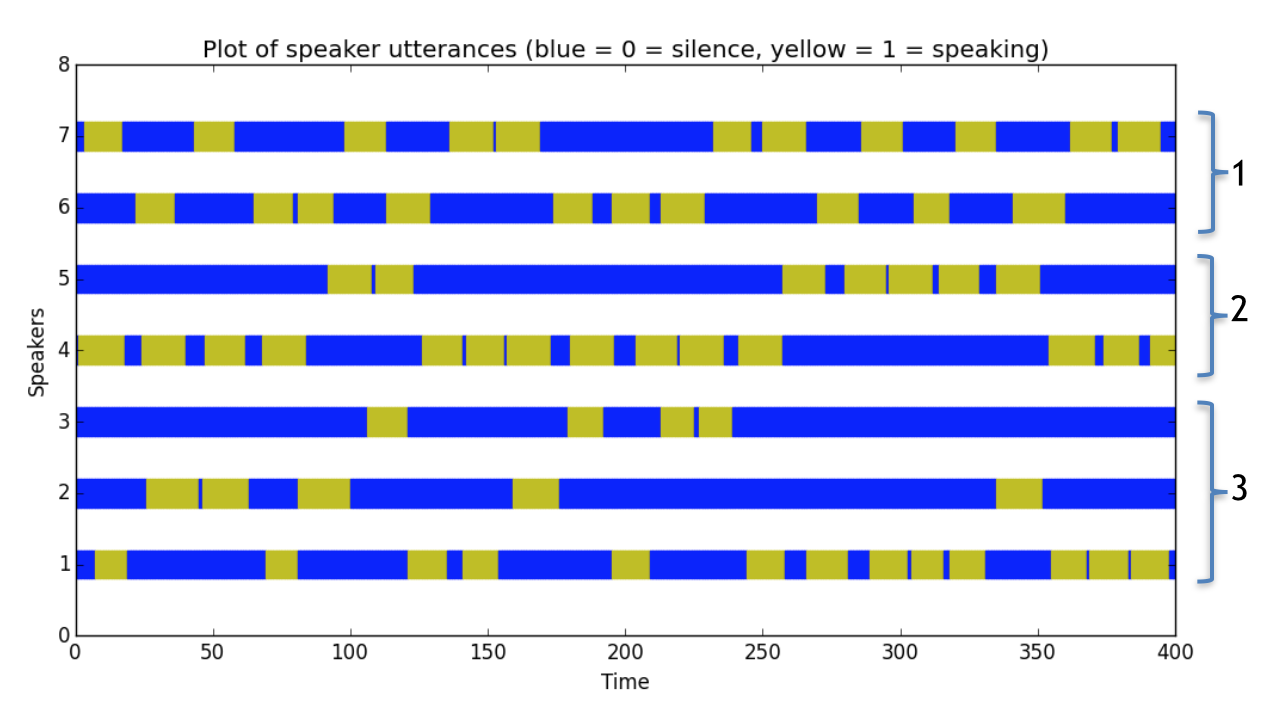
\includegraphics[width=0.8\textwidth]{fig/cocktail-with-groups.png}
  \caption{Example latent binary vector sequence for synthetic
    "cocktail party with conversational groups" data.  Conversational
    groups are indicated by the brackets on the right.}
  \label{fig:cocktail-binary-sequences}
\end{figure}

\paragraph{Synthetic Data}
For the synthetic cocktail party data, the turn sequence within each conversation was
generated using a Hidden Semi-Markov Model (HSMM) with Poisson distributed state-durations, in which the state sequence had $s_c$ states, with pauses with
shorter Poisson duration inserted between each ``sentence''.  The
states within conversations were then mapped to a binary vector with
$s_c$ entries, where silence is represented by all zeroes, 
and speaker $s$ speaking corresponds to a 1 in position $s$.  
The binary vectors were concatenated across
conversations to yield latent states consisting of length $S$ binary
vectors.  To simulate speakers being recorded by $K$ microphones,
weights mapping speakers to microphones were generated independently from
a $U(0,1)$ distribution, resulting in a $D \times K$ weight matrix,
$W$.  A constant ``background sound level'' parameter for each microphone was added as
well, also $U(0,1)$, and independent $\Norm{0}{\sigma^2_k}$ noise was added
to each time step at microphone $k$.

Transition and emission parameters were generated from conjugate priors
to the Poisson HSMM.  The data set
consisted of four conversations of four speakers each, and 12
microphones, so that $D = 16$, and $K = 12$.  There are therefore
$2^{16} = 65536$ possible binary vector-valued states, but only
$(4+1)^4 = 625$, less than 1\%, can actually occur.  The noise variance $\sigma^2_k$ 
was set to a constant of $1/10$ for all $k = 1, \dots, K$.

\paragraph{PASCAL Dataset}
The dataset for this experiment was constructed using a pool of 
500 utterances wasfrom the the PASCAL 1st Speech Separation
Challenge\footnote{\url{http://laslab.org/SpeechSeparationChallenge/}}.
In this data, each ``turn'' within a conversation consists of a single sentence
(average duration $\sim 3$s) and turn orders within a conversation were
randomly generated, with random pauses distributed $\Norm{1/4s}{(1/4s)^2}$
inserted between sentences.  Every time a speaker has a turn, the
sentence is drawn randomly from the 500 sentences uttered by that
speaker in the data.  The conversations continued for 40s, and 
the signal was down-sampled to length 2000.  The 'on' portions of each
speaker's signal were normalized to have amplitudes with mean 1 and standard
deviation 0.5.  An additional column of 1s was added to the speaker signal matrix,
representing background noise.  The resulting signal matrix, $\boldeta$, was thus
$2000 \times 17$ and the weight matrix was $17 \times 12$.  Following
\citet{gael2009infinite} and \citet{valera2015infinite}, the weights
were drawn independently from a $\Unif{0,1}$ distribution, and
independent $\Norm{0}{0.3^2}$ noise was added to each entry of the
observation matrix. 

As with the synthetic data, weights mapping speakers to microphones 
were generated independently from
a $U(0,1)$ distribution, resulting in a $D \times K$ weight matrix,
$W$.  A constant ``background sound level'' parameter for each
microphone was again added,
also $U(0,1)$, and independent $\Norm{0}{\sigma^2_k}$ noise was added
to each time step at microphone $k$.

\paragraph{Results}
The states were inferred from the data using five models: 
(1) a binary-state Factorial HMM, in which the
individual binary speaker sequences are modeled as independent a
priori, (2) an ordinary HDP-HMM without local transitions, where the
latent states are binary vectors, (3) the Sticky HDP-HMM, (4) our
HDP-HMM-LT model, and (5) a model that combines the local transition
property with the ``Sticky'' property: the Sticky HDP-HMM-LT.  
The same linear-Gaussian emission model was employed for all models; 
the only difference was the prior on the sequence of binary state vectors.

To simplify interpretation of the results, the weight matrix
was fixed to the true value (this makes the latent dimensions
identifiable and makes comparisons between inferred and ground truth
state matrices meaningful).  Each model was evaluated at each Gibbs
iteration using the Hamming distance between inferred 
and ground truth state matrices, as well as the F1 score, which is the harmonic mean between the precision (the proportion of the 1s in the inferred state matrix that were actually 1 in the ground truth) and recall (the proportion of the 1s in the ground truth state matrix that were correctly classified as 1 by the model).

The results for the five models on the synthetic and PASCAL datasets are in Figs
\ref{fig:synth-cocktail-results} and \ref{fig:pascal-results},
respectively.  
In Figs \ref{fig:synth-cocktail-binary-matrices} and
\ref{fig:pascal-binary-matrices}, the ground truth state
matrix is shown against the expected state matrix for the five models,
averaged over the 10 runs and all iterations 1001 through 2000.  
The LT and Sticky-LT models outperform the others on all measures. 

The inferred decay rate $\lambda$ for the
HDP-HMM-LT model and its Sticky counterpart on the synthetic and
PASCAL datasets are shown in Figs. \ref{fig:synth-cocktail-results}
and \ref{fig:pascal-results} as well.  Both LT models settle 
on a non-negligible $\lambda$ value for both datasets, suggesting that 
the local transition structure explains the data well.  
They also use more components than the non-LT HDP
models, perhaps owing to the fact that the weaker transition prior of
the non-LT models is more likely to explain nearby similar observations
as a single persisting state, whereas the LT models place a higher
probability on transitioning to a new state with a similar latent vector.

\begin{figure}[tb]
  \centering
  \begin{minipage}{0.75\textwidth}
  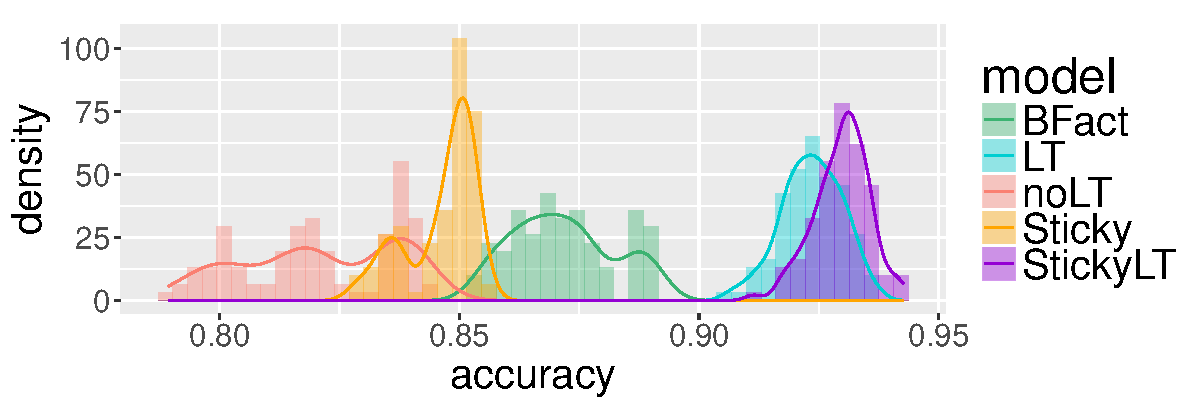
\includegraphics[width = \textwidth]{fig/cocktail/synth_s16_m12/hyper_h/h10.0_nocs_cp0/a5b0p01/accuracy_density.pdf}
\end{minipage}

\begin{minipage}{0.75\textwidth}
  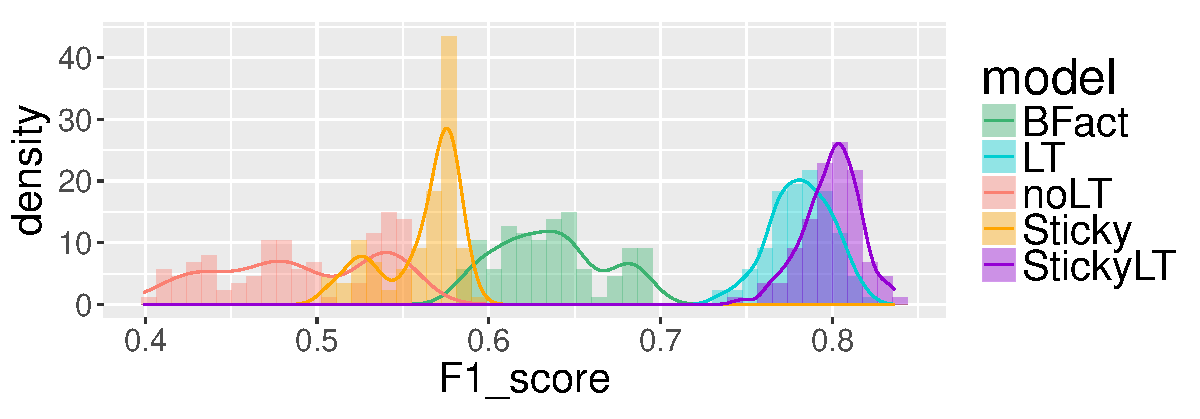
\includegraphics[width = \textwidth]{fig/cocktail/synth_s16_m12/hyper_h/h10.0_nocs_cp0/a5b0p01/F1_score_density.pdf}
\end{minipage}

\begin{minipage}{0.75\textwidth}
  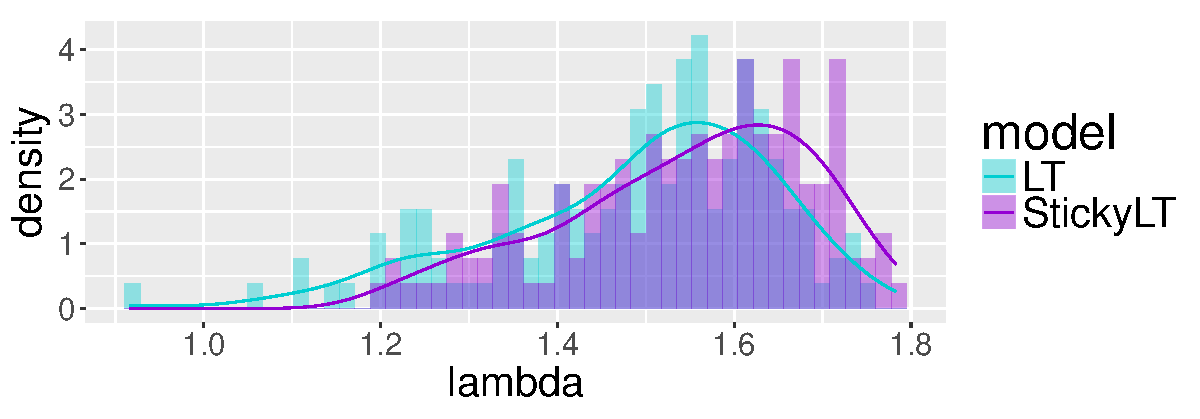
\includegraphics[width = \textwidth]{fig/cocktail/synth_s16_m12/hyper_h/h10.0_nocs_cp0/a5b0p01/lambda_density.pdf}
\end{minipage}

\begin{minipage}{0.75\textwidth}
  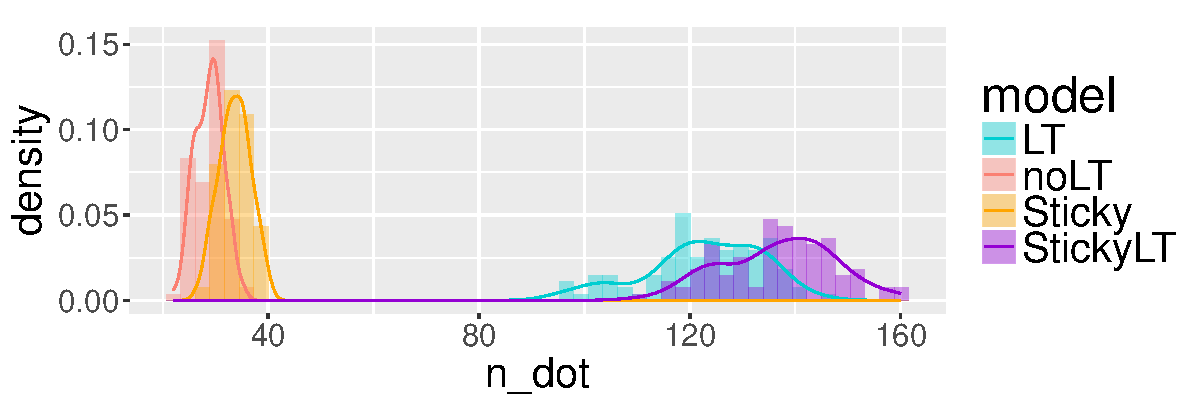
\includegraphics[width = \textwidth]{fig/cocktail/synth_s16_m12/hyper_h/h10.0_nocs_cp0/a5b0p01/n_dot_density.pdf}
\end{minipage}
\caption{(a-b) Accuracy and F1 scores for the HDP-HMM-LT, standard HDP-HMM, and
    Binary Factorial HMM on
    the synthetic cocktail party data.  Metrics are averaged
  over 10 Gibbs runs on each model, with error bars representing a 99\% confidence
  interval for the mean per iteration.  The first 100 iterations are
  not shown. (c) Learned similarity parameter, $\lambda$, for the LT
  model, (d) Number of distinct states used by HDP-HMM and
  HDP-HMM-LT.  The first 100 iterations are excluded.}
  \label{fig:synth-cocktail-results}
\end{figure}

\begin{figure}[tb]
% \vskip 0.1in
\begin{center}
  \centerline{\includegraphics[width = \textwidth, height = 0.2\textwidth]{fig/cocktail/synth_s16_m12/hyper_h/h10.0_nocs_cp0/a5b0p01/groundtruth.pdf}}
  \centerline{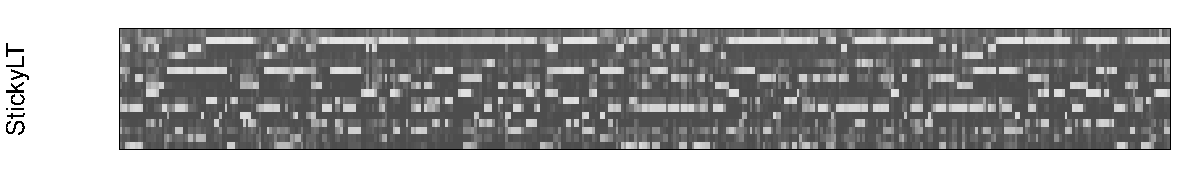
\includegraphics[width = \textwidth, height = 0.2\textwidth]{fig/cocktail/synth_s16_m12/hyper_h/h10.0_nocs_cp0/a5b0p01/StickyLT_hdp_hmm_w0_ah5_bh0p01/binary_state.pdf}}
  \centerline{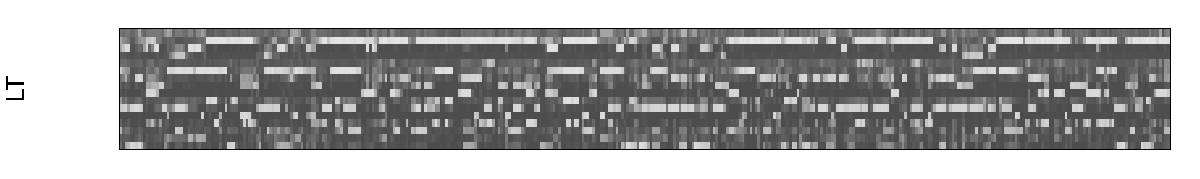
\includegraphics[width = \textwidth, height = 0.2\textwidth]{fig/cocktail/synth_s16_m12/hyper_h/h10.0_nocs_cp0/a5b0p01/LT_hdp_hmm_w0_ah5_bh0p01/binary_state.pdf}}
  \centerline{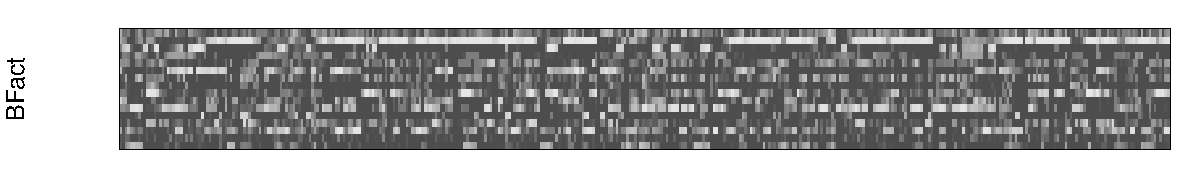
\includegraphics[width = \textwidth, height = 0.2\textwidth]{fig/cocktail/synth_s16_m12/hyper_h/h10.0_nocs_cp0/a5b0p01/BFact_hmm_w0_ah5_bh0p01/binary_state.pdf}}
  \centerline{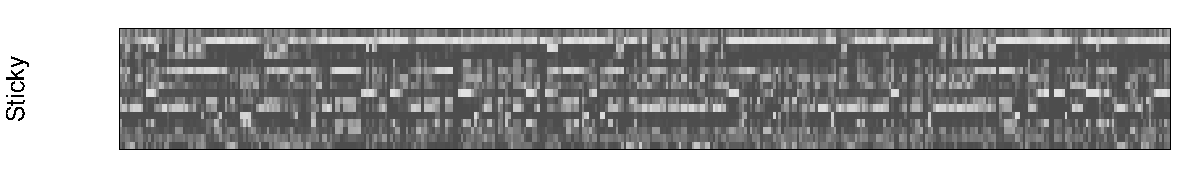
\includegraphics[width = \textwidth, height = 0.2\textwidth]{fig/cocktail/synth_s16_m12/hyper_h/h10.0_nocs_cp0/a5b0p01/Sticky_hdp_hmm_w0_ah5_bh0p01/binary_state.pdf}}
  \centerline{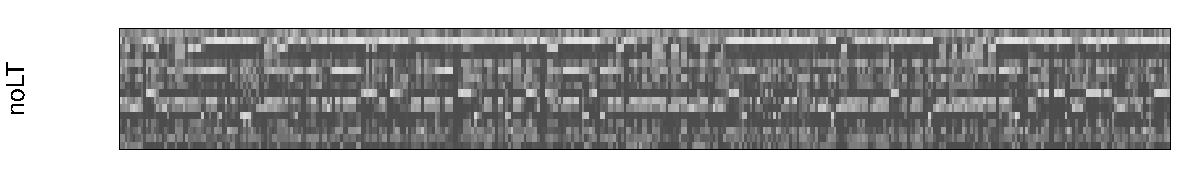
\includegraphics[width = \textwidth, height = 0.2\textwidth]{fig/cocktail/synth_s16_m12/hyper_h/h10.0_nocs_cp0/a5b0p01/noLT_hdp_hmm_w0_ah5_bh0p01/binary_state.pdf}}
\caption{Binary speaker matrices for the synthetic cocktail data, with time on
  the horizontal axis and speaker on the vertical axis.  White is 1,
  black is 0.  The ground truth matrix is at the top, followed by the 
  inferred speaker matrix for the
  Sticky HDP-HMM-LT, HDP-HMM-LT, binary factorial, Sticky-HDP-HMM, and
  ``vanilla'' HDP-HMM.  All inferred matrices are averaged over 5 runs
  of 5000 Gibbs iterations each, with the first 2000 iterations
  discarded as burn-in. \label{fig:synth-cocktail-binary-matrices}}
\end{center}
\end{figure}

\begin{figure}[tb]
  \centering
  \begin{minipage}{0.75\textwidth}
  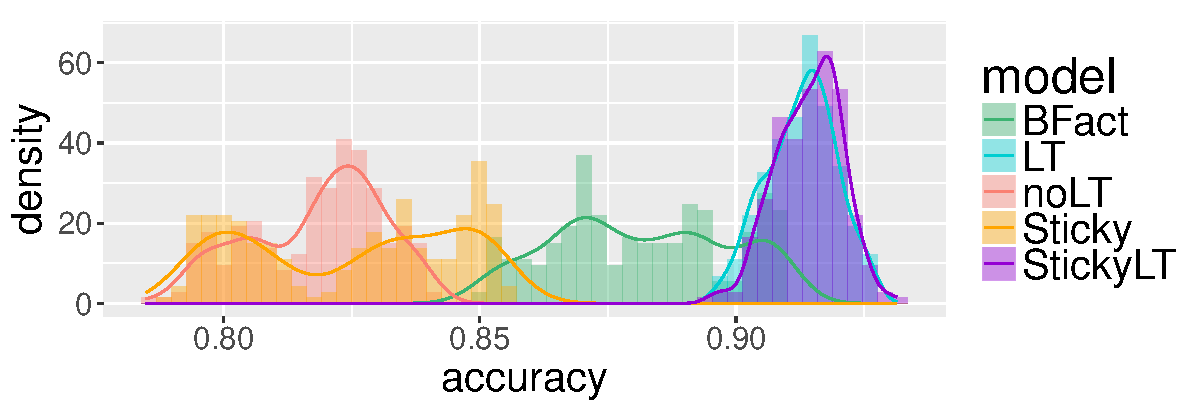
\includegraphics[width = \textwidth]{fig/cocktail/SSC1_s16_m12/abs_2000_n0.3_cp0/all_models/accuracy_density.pdf}
\end{minipage}

\begin{minipage}{0.75\textwidth}
  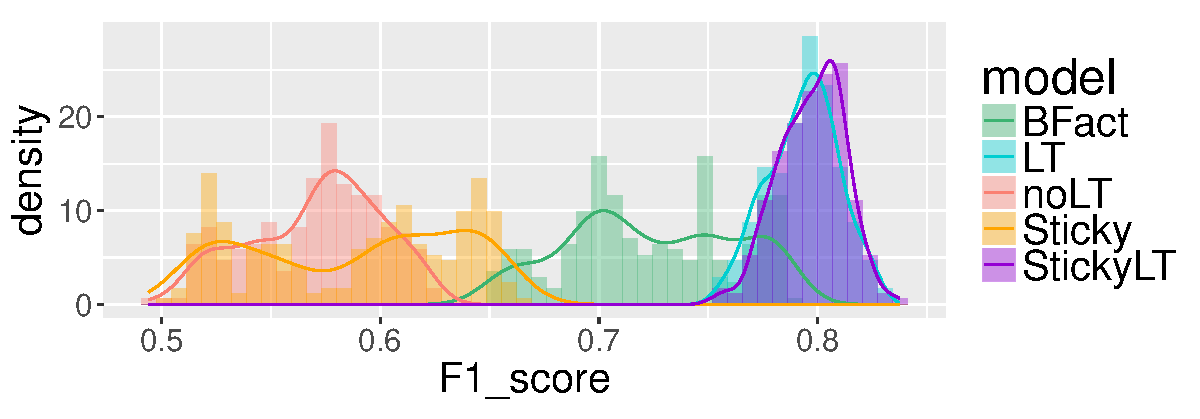
\includegraphics[width = \textwidth]{fig/cocktail/SSC1_s16_m12/abs_2000_n0.3_cp0/all_models/F1_score_density.pdf}
\end{minipage}

\begin{minipage}{0.75\textwidth}
  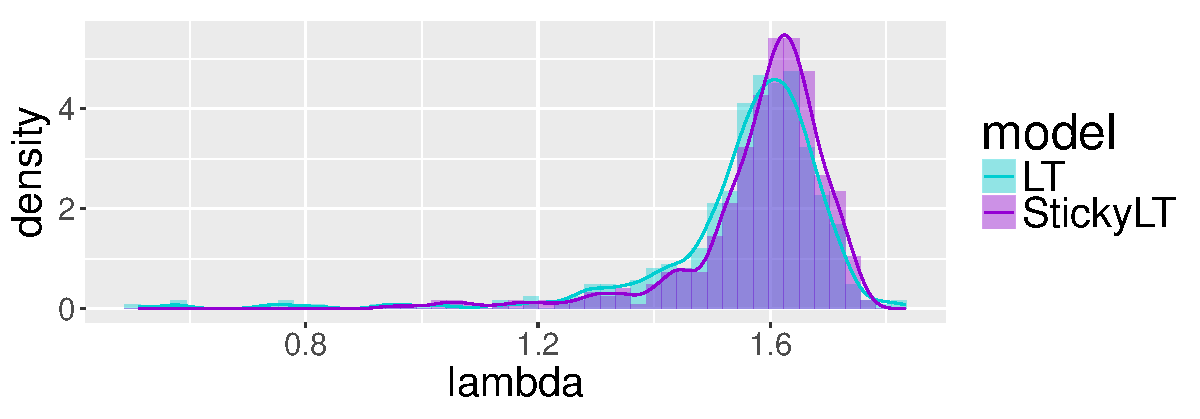
\includegraphics[width = \textwidth]{fig/cocktail/SSC1_s16_m12/abs_2000_n0.3_cp0/all_models/lambda_density.pdf}
\end{minipage}

\begin{minipage}{0.75\textwidth}
  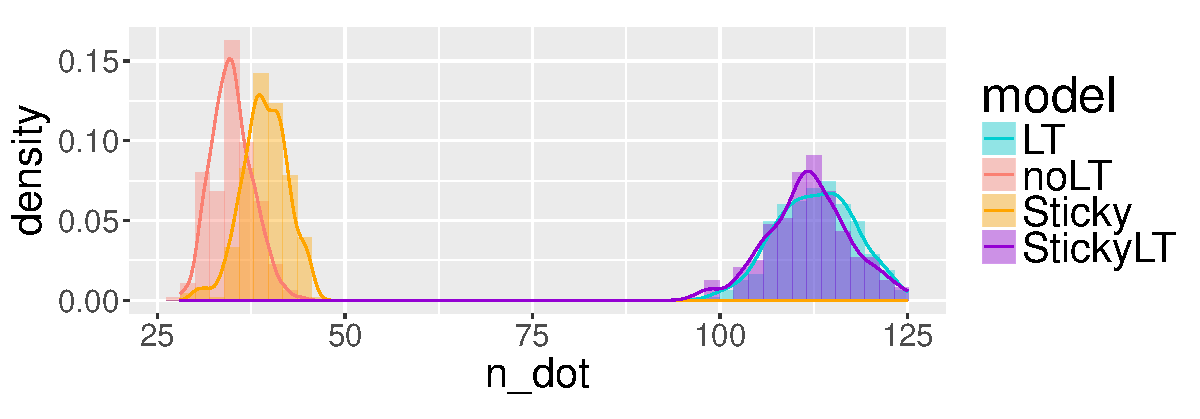
\includegraphics[width = \textwidth]{fig/cocktail/SSC1_s16_m12/abs_2000_n0.3_cp0/all_models/n_dot_density.pdf}
\end{minipage}
\caption{(a-b) Accuracy and F1 scores for the HDP-HMM-LT, standard HDP-HMM, and
    Binary Factorial HMM on
    the PASCAL cocktail party data.  Metrics are averaged
  over 10 Gibbs runs on each model, with error bars representing a 99\% confidence
  interval for the mean per iteration.  The first 100 iterations are
  not shown. (c) Learned similarity parameter, $\lambda$, for the LT
  model, (d) Number of distinct states used by HDP-HMM and
  HDP-HMM-LT.  The first 100 iterations are excluded.}
  \label{fig:pascal-results}
\end{figure}

\begin{figure}[tb]
% \vskip 0.1in
\begin{center}
  \centerline{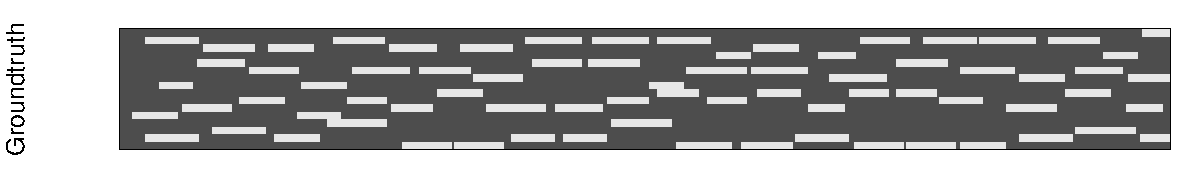
\includegraphics[width = \textwidth, height = 0.2\textwidth]{fig/cocktail/SSC1_s16_m12/abs_2000_n0.3_cp0/all_models/groundtruth.pdf}}
  \centerline{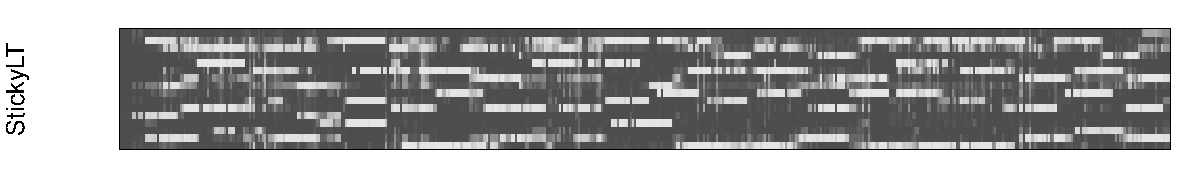
\includegraphics[width = \textwidth, height = 0.2\textwidth]{fig/cocktail/SSC1_s16_m12/abs_2000_n0.3_cp0/all_models/StickyLT_hdp_hmm_w0/binary_state.pdf}}
  \centerline{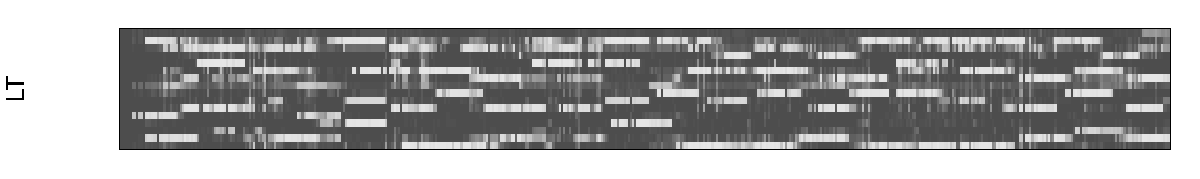
\includegraphics[width = \textwidth, height = 0.2\textwidth]{fig/cocktail/SSC1_s16_m12/abs_2000_n0.3_cp0/all_models/LT_hdp_hmm_w0/binary_state.pdf}}
  \centerline{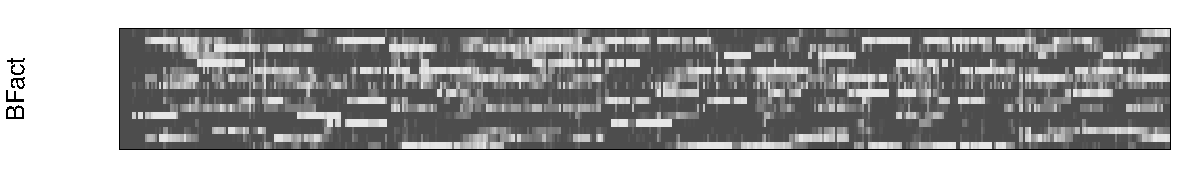
\includegraphics[width = \textwidth, height = 0.2\textwidth]{fig/cocktail/SSC1_s16_m12/abs_2000_n0.3_cp0/all_models/BFact_hmm_w0/binary_state.pdf}}
  \centerline{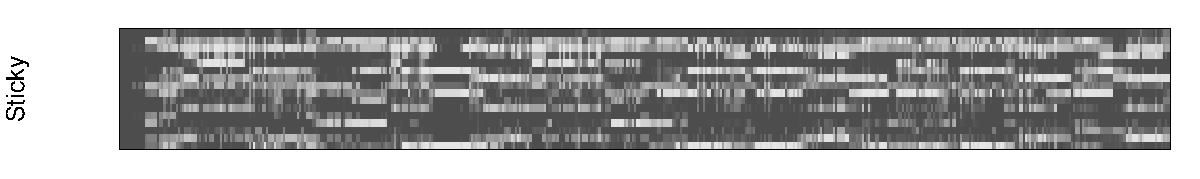
\includegraphics[width = \textwidth, height = 0.2\textwidth]{fig/cocktail/SSC1_s16_m12/abs_2000_n0.3_cp0/all_models/Sticky_hdp_hmm_w0/binary_state.pdf}}
  \centerline{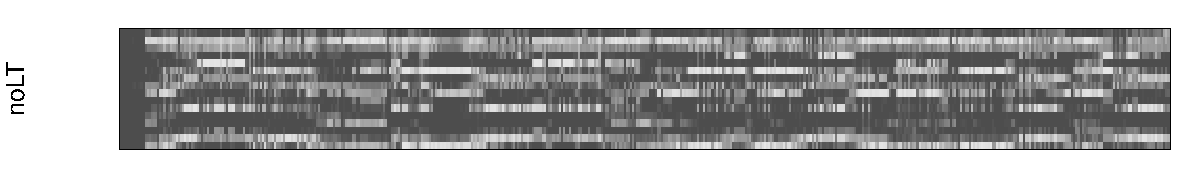
\includegraphics[width = \textwidth, height = 0.2\textwidth]{fig/cocktail/SSC1_s16_m12/abs_2000_n0.3_cp0/all_models/noLT_hdp_hmm_w0/binary_state.pdf}}
\caption{Binary speaker matrices for the PASCAL cocktail party data, with time on
  the horizontal axis and speaker on the vertical axis.  White is 1,
  black is 0.  The ground truth matrix is at the top, followed by the 
  inferred speaker matrix for the
  Sticky HDP-HMM-LT, HDP-HMM-LT, binary factorial, Sticky-HDP-HMM, and
  ``vanilla'' HDP-HMM.  All inferred matrices are averaged over 5 runs
  of 5000 Gibbs iterations each, with the first 2000 iterations
  discarded as burn-in. \label{fig:pascal-binary-matrices}}
\end{center}
\end{figure}

\section{Synthetic Data Without Local Transitions}
\label{sec:synth-data-without}

As a ``sanity check'' on the model, data was also generated 
directly from an ordinary HDP-HMM, with no local
transition property, in order to investigate the performance of our
model in a case where the data did not have the key property that its
prior equipped it to discover.  The results are in
Fig. \ref{fig:synthetic-results}.
During iterations when the $\lambda$ parameter is large, the LT model has worse
performance than the non-LT model on this data, as its bias toward
local transitions is not helpful; however, the
$\lambda$ parameter settles near zero as sampling continues, and the 
model learns that a preference for local transitions does not help to explain
the data.  Note that when $\lambda = 0$, the HDP-HMM-LT reduces to an ordinary HDP-HMM.
Unlike on the cocktail party data, the LT model does not use more
states when the data does not have the LT property.

\begin{figure}[tb]
  \centering
  \begin{minipage}{0.75\textwidth}
  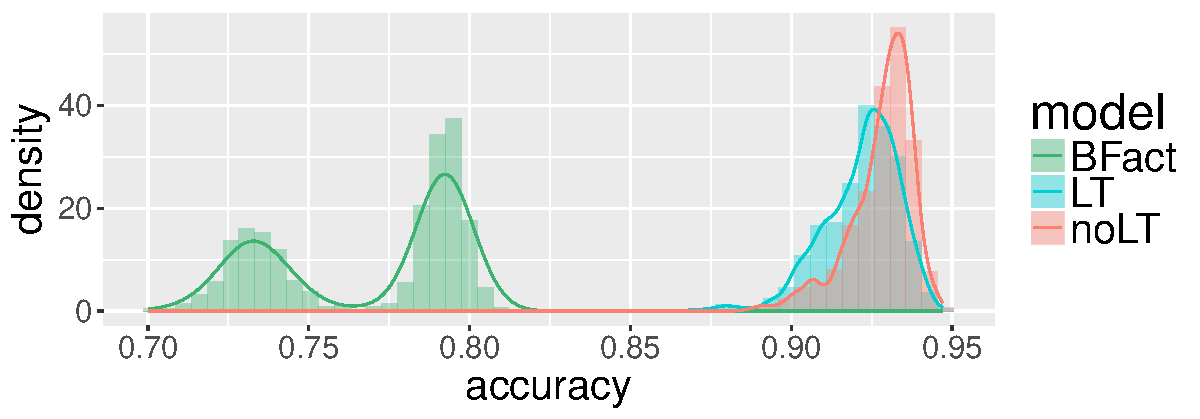
\includegraphics[width = \textwidth]{fig/synth16/accuracy_density.pdf}
\end{minipage}

  \begin{minipage}{0.75\textwidth}
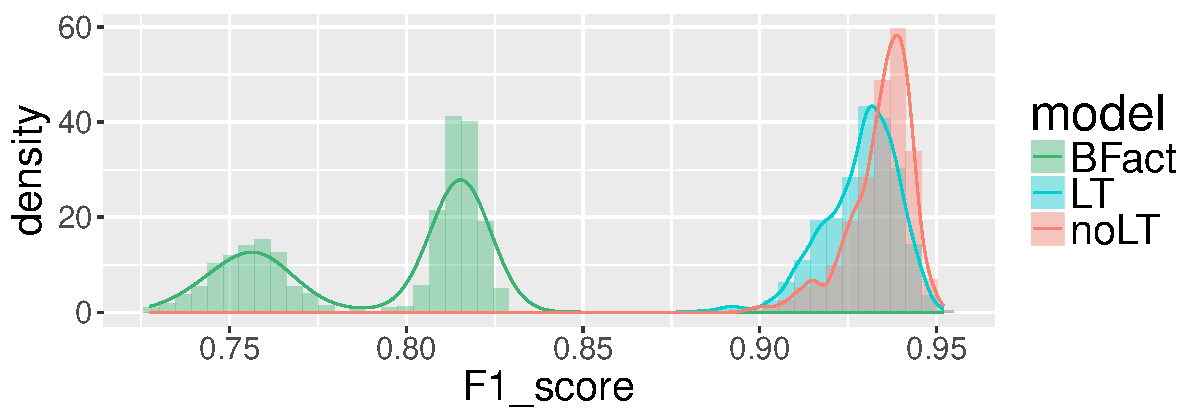
\includegraphics[width = \textwidth]{fig/synth16/F1_score_density.pdf}
\end{minipage}

  \begin{minipage}{0.75\textwidth}
  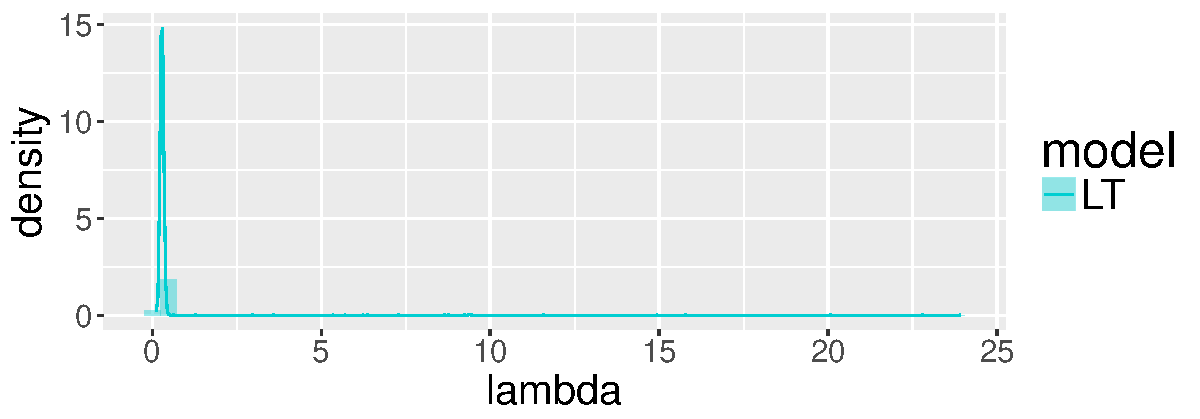
\includegraphics[width = \textwidth]{fig/synth16/lambda_density.pdf}
\end{minipage}

  \begin{minipage}{0.75\textwidth}
  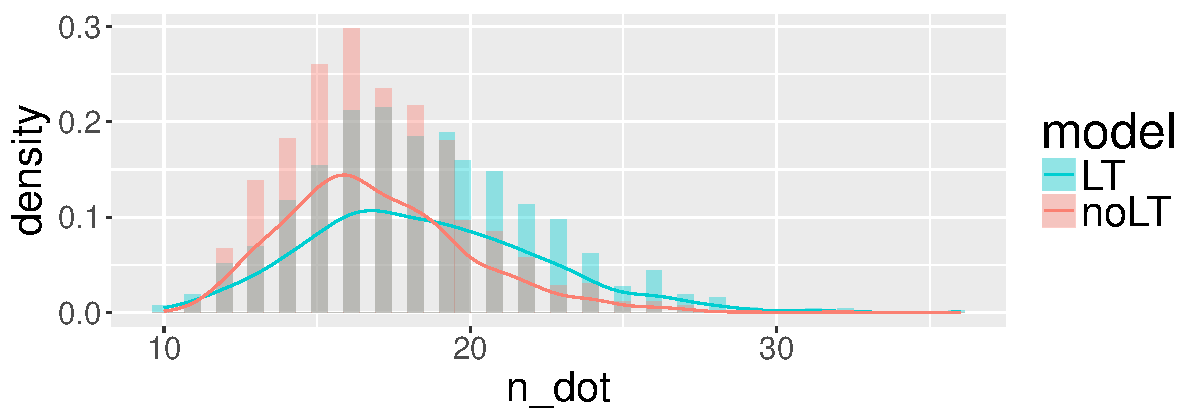
\includegraphics[width = \textwidth]{fig/synth16/n_dot_density.pdf}
\end{minipage}
  \caption{(a-b) Accuracy and F1 for the three models on data generated 
    from an HDP-HMM without local transitions, (c) Learned similarity
    parameter, $\lambda$,
  for the LT model, (d) Number of states used by
  the HDP-HMM and HDP-HMM-LT.  The first 1000 iterations are omitted.}
  \label{fig:synthetic-results}
\end{figure}

\begin{figure}[tb]
% \vskip 0.1in
\begin{center}
  \centerline{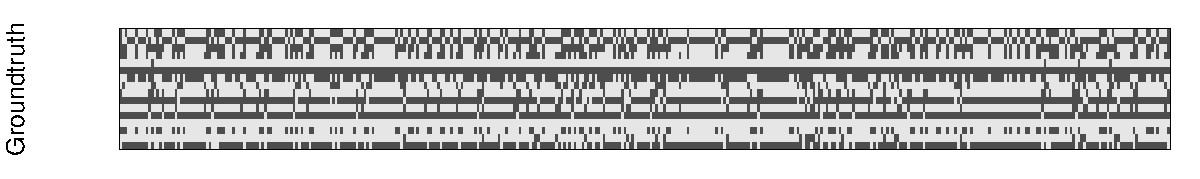
\includegraphics[width = \textwidth, height = 0.2\textwidth]{fig/synth16/groundtruth.pdf}}
  \centerline{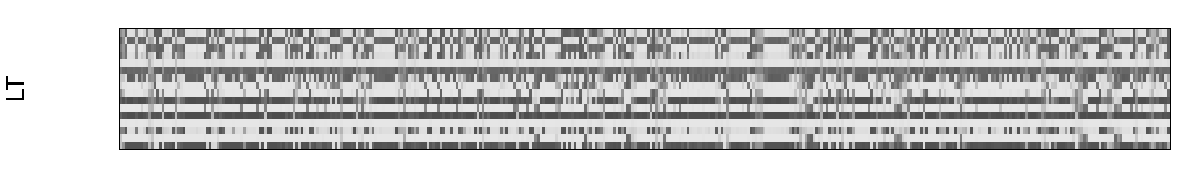
\includegraphics[width = \textwidth, height = 0.2\textwidth]{fig/synth16/LT_hdp_hmm_w0/binary_state.pdf}}
  \centerline{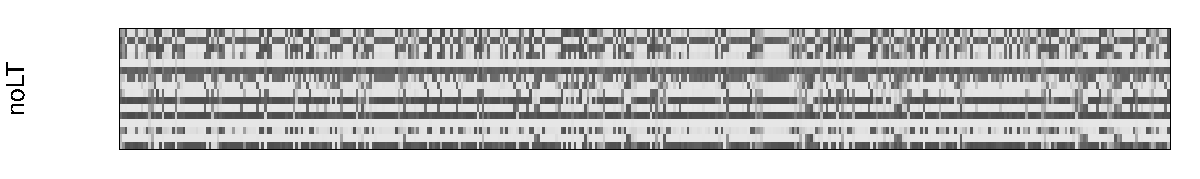
\includegraphics[width = \textwidth, height = 0.2\textwidth]{fig/synth16/noLT_hdp_hmm_w0/binary_state.pdf}}
  \centerline{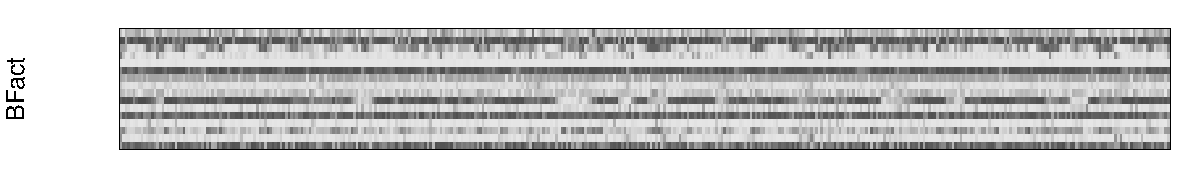
\includegraphics[width = \textwidth, height = 0.2\textwidth]{fig/synth16/BFact_hmm_w0/binary_state.pdf}}
\caption{Binary state matrices for the data generated from a regular HDP-HMM, 
  White is 1, black is 0.  The ground truth matrix is at the top, followed by the 
  inferred speaker matrix for the
  Sticky HDP-HMM-LT, HDP-HMM-LT, binary factorial, Sticky-HDP-HMM, and
  ``vanilla'' HDP-HMM.  All inferred matrices are averaged over 5 runs
  of 2000 Gibbs iterations each, with the first 1000 iterations
  discarded as burn-in. \label{fig:synthetic-binary-matrices}}
\end{center}
\end{figure}

\section{Generalizing to Categorical-Valued $\theta$}
For the experiment described in this chapter, 
we relax the assumption made in Chapter \ref{chapter:cocktail-party} 
that the $\theta_j$ are binary vectors and
instead allow each $\theta_{jd}$ to take on one in an arbitrary set of
discrete values --- i.e., to be categorically distributed rather than
Bernoulli distributed; however the similarity between two states will again be defined in terms of distance between $\theta_j$ vectors that also inform the emission distribution via a linear-Gaussian model.  As a result, much of the additional inference steps described for the 
cocktail party experiment carry over here.  The exception of course is
inferences about $\theta$.

In this chapter, I first define representations and priors for $\theta$ and the weight matrix, 
$W$ for the general case of categorical-vector-valued $\theta$.  Then I derive the necessary Gibbs steps.  Finally, I describe an application to power disaggregation, where the observations consists of an aggregated energy-use time series from several houses, the latent state vector describes the energy being used by each of several channels (e.g., lighting, refrigerator, washer/dryer), such that individual channels are in one of several discrete states at a given time. For example, the refrigerator channel might cycle between an ``off'' state, a low-power standby state, and a high-power ``active cooling'' state.  Inference consists of discovering the set of discrete states for each channel, attributing a typical level of energy consumption for each state, and inferring what state each channel is in during each discretized time window in the data.

\section{Priors and Representations in the Categorical State Variant}
\label{sec:priors-repr-categ}

In place of Beta priors on each $\theta_{jd}$, we use Chinese
Restaurant Process priors, with concentration parameter
$\alpha_{d}^{(\theta)}$.  In the case that the number of categorical 
values is known in advance, this can be replaced by a Dirichlet 
prior, but I present the more flexible case here. 

The weight matrix $W$ must be expanded to allow for distinct weights
associated with each possible value of the $\theta_{jd}$.  Rather than
the matrix given by $(w_{dk})_{d=1,\dots,D,k=1,\dots,K}$, we now need
a set of weights, $(w_{sdk})$, where $s$ indexes the categorical
values that $\theta_{jd}$ can take.  With a CRP prior, 
there is an unbounded number of $s$, though during inference, as in the direct assignment sampler for the HDP-HMM, we need only consider those values to which some state is currently assigned, plus one additional value representing a ``new'' state.

I will continue to assume that the $\phi$ function
decays exponentially as a function of the number of component-wise
differences (that is, Hamming distance) 
between a pair of states.  Specifically, $\Delta_{jj'd}$ is zero
if and only if $\theta_{jd} = \theta_{j'd}$ and is 1 otherwise,
$\Delta_{jj'} = \sum_{d} \Delta_{jj'd}$, and
$\phi(\theta_{j}\theta_{jj'}) = e^{-\lambda\Delta_{jj'}}$.
  
We can use a ``dummy variable'' representation
of $\theta_j$.  Define $S_d$ to be the number of realized
states for dimension $d$ and a 1 in position $\sum_{d' < d} S_{d'} + s$ indicates that
$\theta_{jd} = s$.  There will thus be $D$ entries equal to 1, with
the remaining entries equal to zero.  We can then represent the weight
matrix $\bW$ as stacked block matrix, where each block is $S_d
\times K$, and there is one block for each $d$.  In practice we only
need to instantiate a new block when some $\theta_{jd}$ is assigned to
a ``new table'' in the CRP metaphor, so that the dimension of $\bW$ is
$\sum_d S_d \times K$.  Then we have
\begin{equation}
  y_{t} \sim \Norm{w^{(b)} + W^{\sf T}\theta_{z_t}}{\Sigma}
\end{equation}
where $w^{(b)}$ is a $K$-dimensional bias vector with a separate Normal
prior, $W$ is the weight matrix as defined just above, $z_t$ is the
state indicator for time $t$, and $\Sigma$ is a $K \times K$ noise covariance matrix.

\section{Adapting Posterior Inference for Categorical State Vectors}
\label{sec:adapt-post-infer}

\subsubsection{Sampling $\theta$}

As before, the conditional posterior for $\theta_{jd}$ 
is proportional to the product of three terms: the prior (now a CRP),
the likelihood of all successful and failed transitions to and from
state $j$, and the likelihood of the observation sequence.

Under the CRP, the probability that $\theta_{jd} = s$ conditioned on the rest of $\theta$ (but not the data) is proportional to the number of other $j' \neq j$ such that
$\theta_{j'd} = s$ where this count is positive; and proportional to
$\alpha_j^{(\theta)}$ otherwise.  Let 
\begin{equation}
\tilde{n}^{-j}_{ds} = \sum_{j' \neq j} I(\theta_{jd} = s), \quad s = 1,
\dots, S_d
\end{equation}
be these counts, where we assume that there are $S_d$ distinct values
taken by the $\theta_{jd}$ for a particular $d$.  Then
\begin{equation}
  p(\theta_{jd} = s \given \theta_{d}^{-j}) \propto
\begin{cases}
\tilde{n}^{-j}_{ds} & s = 1, \dots, S_d \\
\alpha_{d}^{(\theta)} & s = S_d + 1
\end{cases}
\end{equation}

The transition component of the likelihood is as in the binary case:
\begin{align}
  p(z, Q \given \theta_{jd}, \theta_{d}^{-j}) & \propto
  e^{-\lambda\sum_{j'} \Delta_{jj'} (n_{jj'} + n_{j'j})} \prod_{j'
    \neq j} (1 - e^{-\lambda\Delta_{jj'} (q_{jj'} + q_{j'j})})\\
  &\propto e^{-\lambda \sum_{j'} I(\theta_{jd} \neq \theta_{j'd})
    (n_{jj'} + n_{j'j})} \prod_{j'
    \neq j} (1 - a\cdot e^{-\lambda I(\theta_{jd} \neq \theta_{j'd}) (q_{jj'} + q_{j'j})})
\end{align}
where $a$ is a constant in $\theta_{jd}$, defined as $e^{-\lambda
  \Delta_{jj'-d} (q_{jj'd} + q_{j'jd})}$.  Taking a log yields
\begin{equation}
  \log p(z, Q \given \theta_{jd}, \theta_{d}^{-j}) =
  -\lambda \sum_{\{j':\ \theta_{jd} \neq \theta_{j'd}\}} (n_{jj'} +
  n_{j'j}) + \sum_{j'
    \neq j} \log(1 - a\cdot e^{-\lambda I(\theta_{jd} \neq \theta_{j'd}) (q_{jj'} + q_{j'j})})
\end{equation}

The emission component of the likelihood is given for each $t$ by
\begin{equation}
  p(y_t \given \theta_{z_t}, W, \Sigma) \propto \abs{\Sigma}^{-1/2}
  \exp(-\frac{1}{2} (y_t - w^{(b)} -
  W^{\sf T} \theta_{z_t})^{\sf T}\bSigma^{-1}(y_t - w^{(b)} - W^{\sf T} \theta_{z_t}))
\end{equation}

Assuming a diagonal covariance matrix, isolating $\theta_{j,d}$, and
taking a log, this becomes, for each $k$ and $t$,
\begin{align}
  \log p(y_{tk} \given \theta_{z_t,d}, \theta_{z_t}^{-d}, w^{(b)}_k, \sigma^2_k) &=
   -\frac{1}{2\sigma^2_k} \left(y_{tk} -
      w^{(b)}_k-\theta_{z_t}\bw_k\right)^2 \\
  &\propto -\frac{1}{2\sigma^2_k} (\sum_{d'} w_{\theta_{z_td'},d',k} -
    (y_{tk} - w^{(b)}_k))^2 \\
  &\propto -\frac{1}{2\sigma^2_k}(w_{\theta_{z_td},d,k} - (y_{tk} -
    w^{(b)}_k - \sum_{d' \neq d} w_{\theta_{z_t,d'},d',k}))^2
\end{align}
For a particular $j$ and $d$, the full emission log likelihood is a sum of
terms like the above, over all $t$ such that $z_t = j$.

\paragraph{Sampling $W$}
Having expanded $\theta$ to a dummy variable representation, and
having constructed a stacked block form of $W$, we can sample each
column of $W$ from a conditional posterior multivariate Normal just
as in the binary case.

\paragraph{Sampling $\lambda$} Since $\lambda$ controls only the relationship between the distance matrix, $\Delta$, and the similarity matrix, $\phi$, upon 
conditioning on $\Delta$ and the jump attempts, $\lambda$ is not sensitive to the way that $\Delta$ was computed; hence it can be sampled using Adaptive Rejection Sampling from exactly the same conditional distribution as before.

\section{Power Disaggregation}
\label{sec:power-disaggregation}

The categorical model was tested using a subset of the Reference Energy Disaggregation Data set (REDD; \citet{kolter2011redd}).  The data consists of power consumption measurements from several time intervals from several electrical channels in several different homes, as well as an aggregated power consumption time series for each interval per home. An example interval is shown in Fig. \ref{fig:redd-data-example}.  

Two key properties of this data are apparent in the figure.  First, up to some small-scale variability, each channel visits a relatively small number of amplitudes, with some (such as the oven) alternating between an ``on'' state and an ``off'' state, and others (such as the outlets and lighting channels) exhibiting more complex dynamics, presumably corresponding to various appliances or light fixtures turning on and off in different combinations.  This property motivates the choice of a categorical state model.  Second, there are clear correlations among the various channels: in this example, the two oven channels always go on and off together, albeit exhibiting different amplitudes when on, while two of the three lighting channels are highly but not perfectly correlated, while the third exhibits opposing behavior to the other two (perhaps arising from behavior).

Collectively, the dynamics exhibited here are similar to the cocktail party data described in Chapter \ref{chapter:cocktail-party}.  For one, since transitions between combinatorial states tend to be ``local'', in that it is rare for more than one channel to change state at one time, we would expect the HaMMLeT model's bias toward local state transitions to be beneficial, compared to the ``vanilla'' HDP-HMM which has no such locality bias.  On the other hand, not all combinations of states occur in the data, and morever, some state combinations are more or likely than the product of the individual channel probabilities would suggest, suggesting that the flexibility of a model such as HaMMLeT, in which there is a single latent state space over vector-valued states, might be better able to capture the correct transition probaiblities than a model such as the Factorial HMM, in which the component chains evolve {\em a priori} independently.

\begin{figure}[tb]
  \centering
  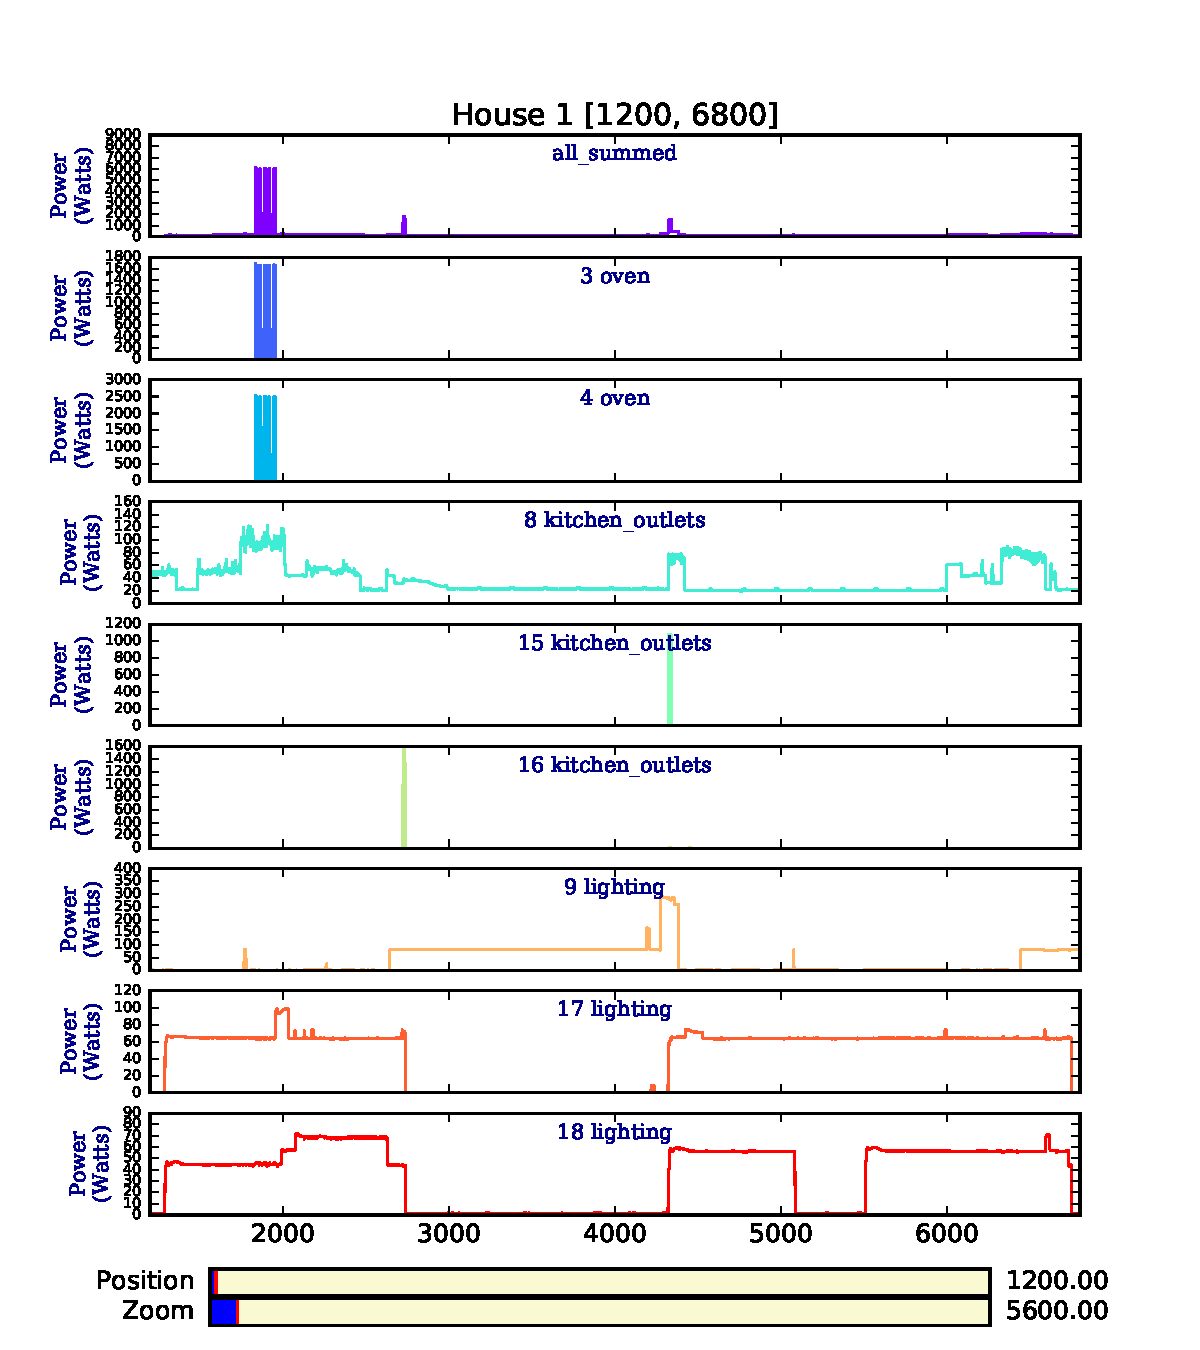
\includegraphics[width=\textwidth]{data/REDD/jw2013_downsampled_intervals/house_1_1200_6800/house_1_1200-6800.pdf}
  \caption{A sample data interval from the REDD dataset \cite{kolter2011redd}.  The top channel contains the total measured power in watts consumed by a home during a period of approximately 24 hours.  Each timestep represents a 20 second intervals, during which the amplitude recorded is a median of the amplitudes in the original higher resolution data.}
  \label{fig:redd-data-example}
\end{figure}

% \chapter{\MakeUppercase{Categorical Vector States: Power Disaggregation}}
% \label{chapter:REDD}

\chapter{\MakeUppercase{Separate Similarities and Emissions: Learning
  Tonal Grammar in Music}}
\label{chapter:music}
\section{Separable Similarity and Emissions}
\label{sec:separ-simil-emiss}

In the HDP-HMM-LT model, we have a defined set of states with 
locations $\ell_j$, $j = 1, \dots,
J$.  In Chapters \ref{chapter:cocktail-party} and \ref{chapter:REDD}, the similarities depended on the same parameters that determined the emission distributions, which we denoted by $\theta_j$.  In Chapter \ref{chapter:cocktail-party},
each $\theta_j$ was a binary state vector, and the similarity $\phi_{jj'}$ was a decreasing function of the distance between those state vectors, while the emission distribution was a Gaussian centered at a linear function of $\theta_j$.  In Chapter \ref{chapter:REDD}, we generalized from binary state vectors to categorical state vectors, but similarity was still based on the distance between state vectors, and emission distributions were still Gaussians centered at a linear function of the state vector.

In this chapter, we suppose instead that $\ell_{j}$ consists of two separate and a priori independent parts: $\ell_j = (\theta_{j}, \eta_{j})$, where the $\theta_j$ govern the emission distributions, and the similarities, $\phi_{jj'}$ depend on the $\eta_j$

Define
\begin{equation*}
  \phi_{jj'}(\eta_j, \eta_{j'}) = \exp\left(-\frac{\lambda}{2} \Delta_{jj'}^2\right)
\end{equation*}
where $\Delta_{jj'}$ is the Euclidean distance between $\eta_j$ and
$\eta_{j'}$; that is,
\begin{equation*}
  \Delta_{jj'}^2 = \sum_{d} (\eta_{jd} - \eta_{j'd})^2
\end{equation*}

\section{A Hamlitonian Monte Carlo step to sample $\eta$}
\label{sec:haml-monte-carlo}

Since the $\eta_j$ are real-valued vectors, we can sample them jointly using Hamiltonian Monte Carlo (HMC, also known as ``Hybrid Monte Carlo''; \citet{duane1987hybrid}, see also \citet{neal2011mcmc}).  HMC is a variation on the Metropolis-Hastings MCMC 
algorithm which is designed to more efficiently explore a high-dimensional continuous distribution by adopting a proposal distribution which is based on the evolution of Hamiltonian dynamics in a physical system.  The position of the particle in the system represents the current state of the Markov chain, the potential energy of the particle is the negative log of the target distribution, and an auxiliary ``momentum'' variable is introduced, representing the kinetic energy of the system.  The Markov chain evolves by computing a discrete approximation of an update to the position and momentum variables, and then computing the standard Metropolis-Hastings acceptance probability.

In order to carry out HMC in the context of the HaMMLeT model with latent continuous state variables given by $\eta_j$, $j = 1, \dots, J$, we need the log likelihood and log prior for the $\eta$ vector.  Assume independent and isotropic Gaussian priors on each 
$\eta_{j}$, so we have
\begin{equation*}
  p(\eta_j) \propto \exp\left(-\frac{h_\eta}{2} \sum_{d} \eta_{jd}^2 \right),
\end{equation*}
where $h_{\eta}$ is the prior precision which does not depend on $d$.

Then the log prior density, up to a constant, is
\begin{equation*}
  \log p(\eta_j) \propto -\frac{h_{\eta}}{2} \sum_{d} \eta_{jd}^2
\end{equation*}

The relevant log likelihood, as shown in Chapter \ref{chapter:HaMMLeT} is
the probability of the $z$ and $Q$ variables given the
$\phi_{jj'}$.  In particular, we have
\begin{equation*}
  L := p(\bz, \bQ \given \bphi) = \prod_{j} \prod_{j'} \phi_{jj'}^{n_{jj'}}(1 - \phi_{jj'})^{q_{jj'}}
\end{equation*}
and
\begin{equation*}
  \log L = \sum_{j} \sum_{j'} \left( n_{jj'} \log(\phi_{jj'}) +
    q_{jj'} \log(1 - \phi_{jj'})\right)
\end{equation*}

To do Hamiltonian Monte Carlo to sample from the conditional posterior
of $\eta$ given $\bz$ and $\bQ$, we need to compute the gradient of the
log posterior, which is just the sum of the gradient of the log prior
and the gradient of the log likelihood.

The $j,d$ coordinate of the gradient of the log prior is simply
\begin{equation*}
  -2h_{\eta} \eta_{jd}
\end{equation*}

To get the $j,d$ coordinate of the gradient of the log likelihood, we
can apply the chain rule to terms as is convenient.  In particular,

\begin{equation*}
  \frac{\partial L}{\partial \eta_{jd}}=\sum_{j} \sum_{j'} n_{jj'}
  \frac{\partial \log(\phi_{jj'})}{\partial \Delta_{jj'}^2}
  \frac{\partial \Delta_{jj'}^2}{\partial \eta_{jd}}+ \sum_{j}
  \sum_{j'} q_{jj'} \frac{\partial \log(1 - \phi_{jj'})}{\partial (1 -
    \phi_{jj'})}\frac{\partial (1 - \phi_{jj'})}{\partial
    \Delta_{jj'}^2} \frac{\partial \Delta_{jj'}^2}{\partial \eta_{jd}}
\end{equation*}

We have the following components:
\begin{align*}
  \frac{\partial \log(\phi_{jj'})}{\partial \Delta_{jj'}^2} &=
  -\frac{\lambda}{2} \\
  \frac{\partial \Delta_{jj'}^2}{\partial \eta_{jd}} &= 2\Delta_{jj'd} I(j \neq j')\\
  \frac{\partial \log(1 - \phi_{jj'})}{\partial (1 -
    \phi_{jj'})} &= \frac{1}{1 - \phi_{jj'}} \\
  \frac{\partial (1 - \phi_{jj'})}{\partial
    \Delta_{jj'}^2} &= \frac{\lambda}{2} \phi_{jj'}
\end{align*}
which yields
\begin{align*}
  \frac{\partial L}{\partial \eta_{jd}} &= -\lambda \sum_{j}
  \sum_{j'} n_{jj'} \Delta_{jj'd} \mathbb{I}(j \neq j') +
  \lambda \sum_{j}\sum_{j'} q_{jj'} \Delta_{jj'd} \frac{\phi_{jj'}}{1 -
    \phi_{jj'}} \mathbb{I}(j \neq j) \\
  &= - \lambda \sum_{(j,j'): j \neq j'} \Delta_{jj'd} \left(n_{jj'} - q_{jj'}
    \frac{\phi_{jj'}}{1 - \phi_{jj'}}\right)
\end{align*}
\begin{equation*}
  p(\eta_j) \propto \exp\left(-\frac{h_\eta}{2} \sum_{d} \eta_{jd}^2 \right),
\end{equation*}
where $h_{\eta}$ is the prior precision which does not depend on $d$.

\section{Synthetic Data from an HMM with a Nearly Block Diagonal Transition Matrix}
\label{sec:synthetic-data-from}


\subsection{Data-generation}

As a first check on this version of the model, several datasets were generated from fixed state Hidden Markov models whose transition matrices were close to block-diagonal.  Specifically, the state space consisted of 40 states in total which were grouped into 10 ``superstates'' of 4 states each.  With probability 0.95, the chain transitioned to another state in the same superstate, and with probability 0.05 it transitioned to a different superstate.  The distribution across the 4 same-superstate entries was drawn for each row from a symmetric Dirichlet, where the concentration parameter varied across datasets.  The distribution for each row across the 8 other-superstate entries was drawn from a symmetric Dirichlet as well, where again, the concentration parameter was varied.

Each of the forty states was associated with a mean in a two-dimensional observation space.  However, unlike in the experiments discussed in Chapters \ref{chapter:cocktail-party} and \ref{chapter:REDD}, there was no relationship between proximity in transition space and proximity in emission space: the means for the twelve states were drawn independently from a $\Norm{0}{\sigma^2 I}$ distribution, where $\sigma^2$ was varied across datasets.

At each time step, an observation was drawn from a bivariate $\Norm{\mu_j}{I}$ distribution.

Since the HaMMLeT model infers a latent location for each state, and since the latent state locations impact the transition matrix by promoting transitions between nearby states and suppressing transitions between far away states, it is predicted that the HaMMLeT model will locate states in the same superstate near each other, and so we should expect to see a ``clustering'' of states into three distinct groups based on their $\eta_j$ vectors.  This clustering ability should allow HaMMLeT to more efficiently learn the correct transition matrix as compared to the HDP-HMM with no preference for local transitions.

To evaluate the performance of HaMMLeT versus the ordinary HDP-HMM, each models' calculated marginal log likelihood was computed based on both the training data set used during inference, and on a held-out test set.  At each Gibbs iteration, the marginal log likelihood was computed by fixing the transition matrix and emission parameters, and integrating out the state sequence using the forward message passing algorithm.

\subsection{Results}

\begin{figure}
\begin{minipage}{0.45\textwidth}
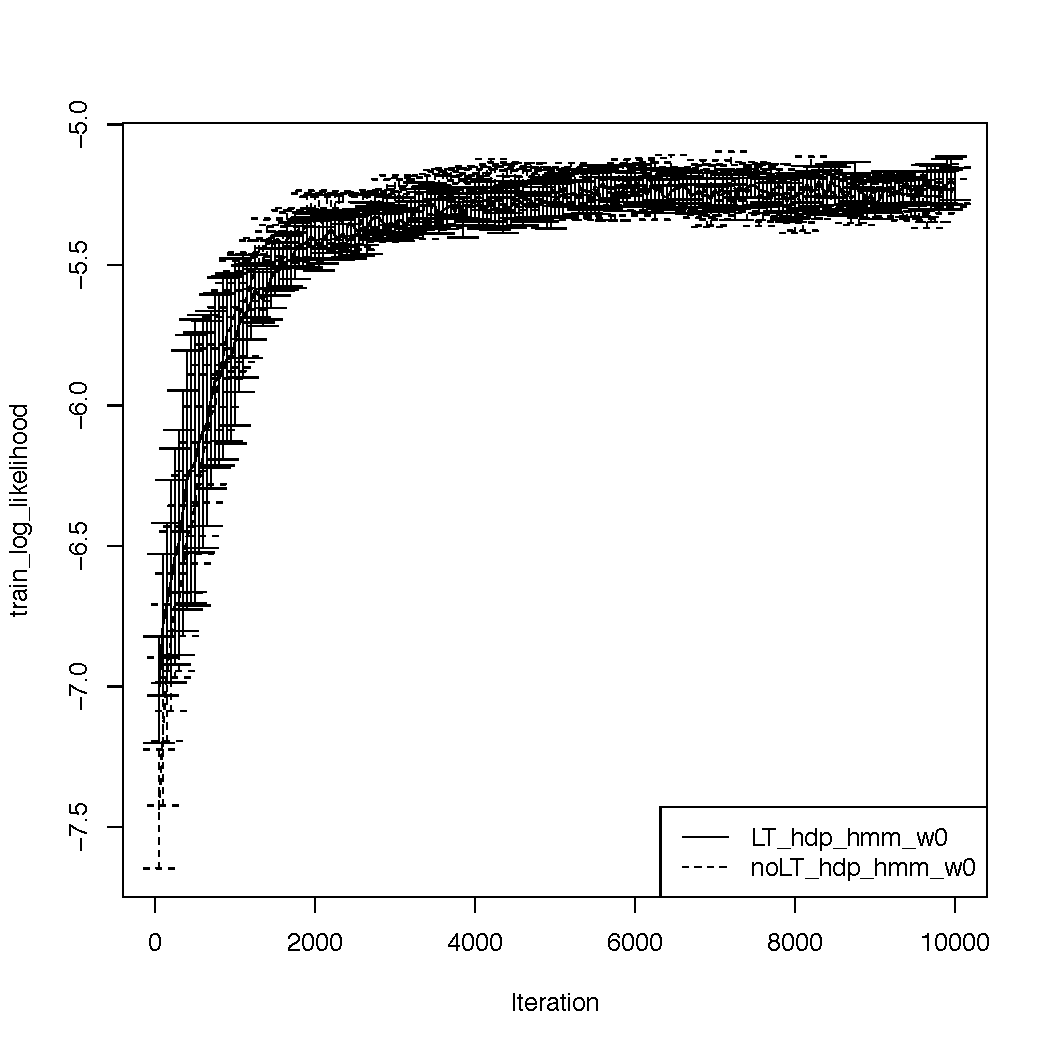
\includegraphics[width=\textwidth]{fig/block_diag/train_log_likelihood}
\end{minipage}
\hspace{0.1in}
\begin{minipage}{0.45\textwidth}
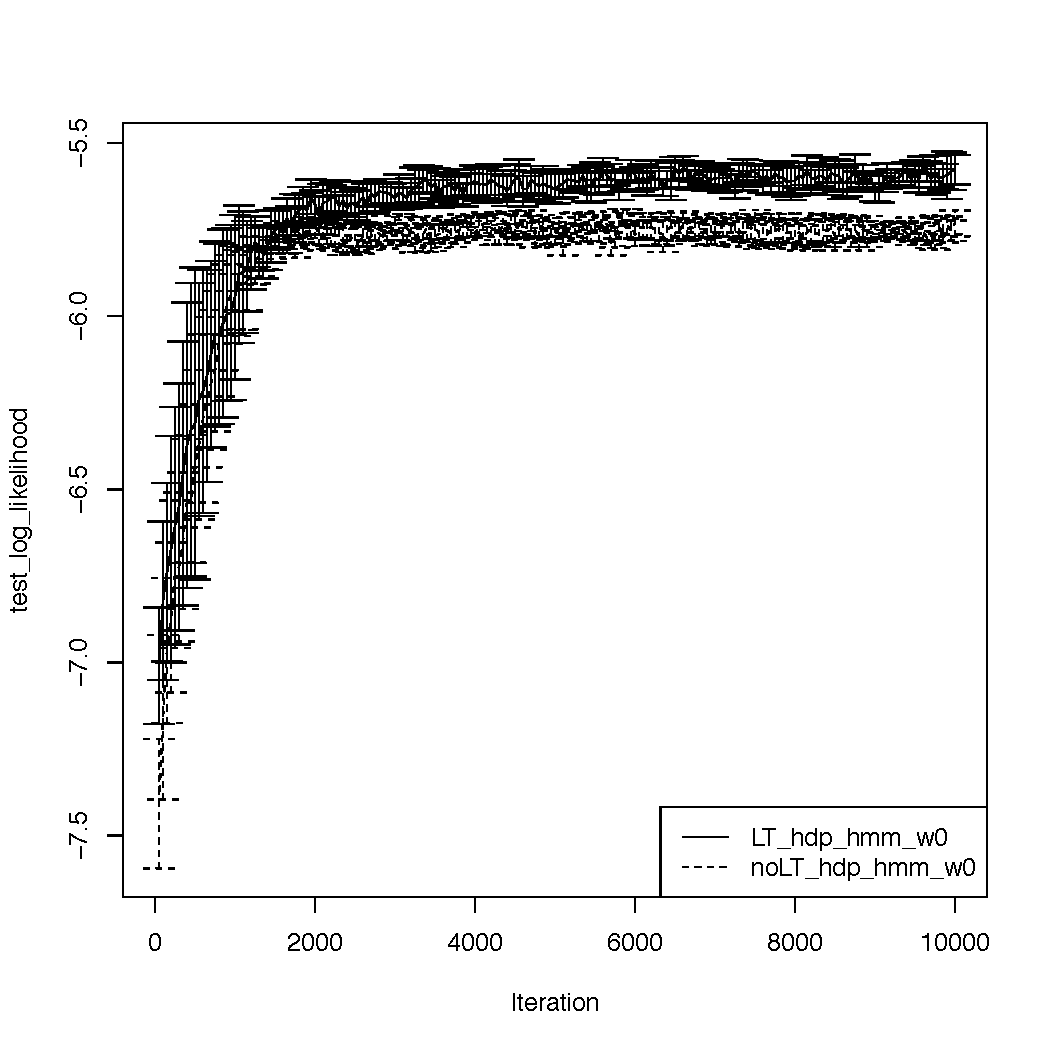
\includegraphics[width=\textwidth]{fig/block_diag/test_log_likelihood}
\end{minipage}
\caption{Left: Log likelihood on the training set by Gibbs iteration
  (marginalizing out state sequence) for LT and no LT (HDP-HMM)
  models.  Right: Log likelihood on a held out test set.}
\end{figure}

\section{Discovering Chord Equivalence Classes in Tonal Music}
\label{sec:disc-chord-equiv}

A real-world test of the separable-similarity form of HaMMLeT comes from the music domain.  We employed a dataset in which each observation consisted of four musical tones played concurrently, constituting a chord, and where the sequences between chords followed conventions for Western tonal music. 

\chapter{\MakeUppercase{Conclusions and Future Work}}
\label{chapter:discussion}

\section{Summary}
\label{sec:summary}

In this dissertation I have presented a new probability model for sequence data: the Hierarchical Dirichlet Process Hidden Markov Model with Local Transitions (HDP-HMM-LT, or ``HaMMLeT''), which provides a way to infer a latent state sequence underlying time series data while incorporating prior information that the latent states reside in some similarity space, with transitions being more likely between pairs of states that are nearby in that space.  Two broad versions of the model are presented, which represent similarity fundamentally differently.  

The first version of the model, illustrated in Chapter \ref{chapter:cocktail-party} conceives of similarity as a function of the emission distributions of the respective states; or at least, of a function of the same state information that influences the emission distributions.  This form of the model is well suited to scenarios in which the latent state is a composite of several component sub-states, not all of which change at the same time; that is, the kinds of settings where factorial models are typically used.  The difference between the HaMMLeT model and a facotrial model is that the substates are not modeled as independent sequences in HaMMLeT, and so it is possible to discover correlations among them.  The performance of this model is illustrated in a speaker diarization experiment (the ``cocktail party'' problem), with favorable comparison to both the ``vanilla'' HDP-HMM and the factorial HMM, whose features it combines, as well as to the Sticky HDP-HMM, which privileges self-transitions but possesses no notion of proximity between non-identical states.

The second version of the model, illustrated in Chapter \ref{chapter:music}, represents similarity between states as unrelated to emissions themselves, which is suited to applications where there is a notion of ``functional distance'' between states which is separate from the surface distance between observations at those states, as is arguably the case in Western music, where the ``circle of fifths'' structures harmonic classes in a manner such that consecutive chords tend to be nearby in the circle, even if their pitches are far apart.  This model is illustrated using two harmonic parsing experiments, one using synthetically generated data from the Kulitta grammar \cite{quick2014kulitta}, and the other using Bach chorales.  Comparisons are made to the vanilla HDP-HMM and the Sticky HDP-HMM.  Here, the key finding is that although the two ``non-LT'' models fit the training data well (in fact better than the LT model), they appear to overfit, yielding worse predictive likelihood on a held out test set than the LT model, which evidently recovers a more parsimonious description of the harmonic structure.

I conclude this dissertation by describing some directions for future work extending and further exploring the properties of the HaMMLeT model.  First I describe a potential application related to power disaggregration, which has been a use case for existing nonparametric Bayesian HMMs (e.g., \cite{johnson2013bayesian}).  Then I describe a possible marriage between the local transition property of HaMMLeT with the nonparametric infinite factorial HMM \cite{gael2009infinite}.  Finally, I discuss computational challenges for inference with the HaMMLeT model, and potential directions for improving scalability.


\section{Future Application: Power Disaggregation}
\label{sec:power-disaggregation}

A potential application of the categorical-vector-state model described in Chapter \ref{chapter:cocktail-party} is to disaggregating energy signals.  In the future, I plan to test the model using a subset of the Reference Energy Disaggregation Data set (REDD; \citet{kolter2011redd}).  The data consists of power consumption measurements from several time intervals from several electrical channels in several different homes, as well as an aggregated power consumption time series for each interval per home. An example interval is shown in Fig. \ref{fig:redd-data-example}.  

Two key properties of this data are apparent in the figure.  First, up to some small-scale variability, each channel visits a relatively small number of amplitudes, with some (such as the oven) alternating between an ``on'' state and an ``off'' state, and others (such as the outlets and lighting channels) exhibiting more complex dynamics, presumably corresponding to various appliances or light fixtures turning on and off in different combinations.  This property motivates the choice of a categorical state model.  Second, there are clear correlations among the various channels: in this example, the two oven channels always go on and off together, albeit exhibiting different amplitudes when on, while two of the three lighting channels are highly but not perfectly correlated, while the third exhibits opposing behavior to the other two (perhaps arising from behavior).

Collectively, the dynamics exhibited here are similar to the cocktail party data described in Chapter \ref{chapter:cocktail-party}.  For one, since transitions between combinatorial states tend to be ``local'', in that it is rare for more than one channel to change state at one time, we would expect the HaMMLeT model's bias toward local state transitions to be beneficial, compared to the ``vanilla'' HDP-HMM which has no such locality bias.  On the other hand, not all combinations of states occur in the data, and morever, some state combinations are more or likely than the product of the individual channel probabilities would suggest, suggesting that the flexibility of a model such as HaMMLeT, in which there is a single latent state space over vector-valued states, might be better able to capture the correct transition probaiblities than a model such as the Factorial HMM, in which the component chains evolve {\em a priori} independently.

\begin{figure}[tb]
  \centering
  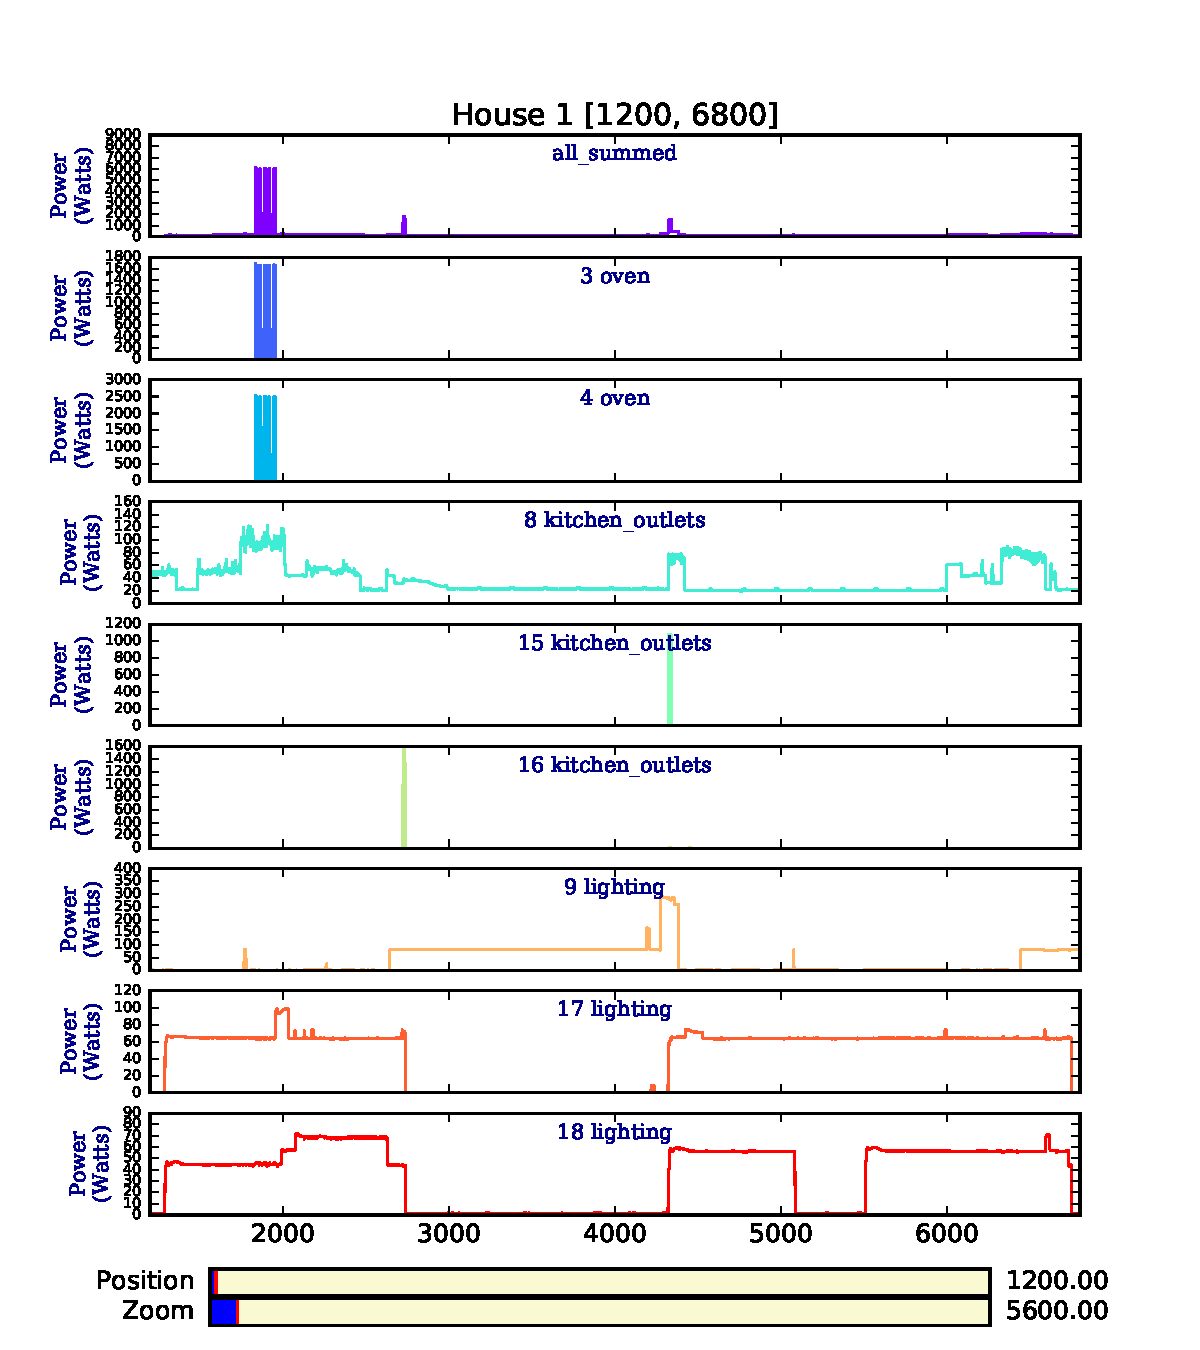
\includegraphics[width=\textwidth]{data/REDD/jw2013_downsampled_intervals/house_1_1200_6800/house_1_1200-6800.pdf}
  \caption{A sample data interval from the REDD dataset \cite{kolter2011redd}.  The top channel contains the total measured power in watts consumed by a home during a period of approximately 24 hours.  Each timestep represents a 20 second intervals, during which the amplitude recorded is a median of the amplitudes in the original higher resolution data.}
  \label{fig:redd-data-example}
\end{figure}

\subsection{Generalizing to Categorical-Valued $\theta$}
It is not difficult to relax the assumption made in Chapter \ref{chapter:cocktail-party} 
that the $\theta_j$ are binary vectors and
instead allow each $\theta_{jd}$ to take on one in an arbitrary set of
discrete values --- i.e., to be categorically distributed rather than
Bernoulli distributed.  The similarity between two states will again be defined in terms of distance between $\theta_j$ vectors that also inform the emission distribution via a linear-Gaussian model.  As a result, much of the additional inference steps described for the 
cocktail party experiment carry over to this instantiation of the
model.  The exception of course is
inferences about $\theta$.

In this section, I define representations and priors for $\theta$ and the weight matrix, 
$W$ for the general case of categorical-vector-valued $\theta$.  Then
I derive the necessary Gibbs steps.  

A potential future application of this version of the model to power
disaggregation is described in Chapter \ref{chapter:discussion}, where the observations consist of an aggregated energy-use time series from several houses, the latent state vector describes the energy being used by each of several channels (e.g., lighting, refrigerator, washer/dryer), such that individual channels are in one of several discrete states at a given time. For example, the refrigerator channel might cycle between an ``off'' state, a low-power standby state, and a high-power ``active cooling'' state.  Inference consists of discovering the set of discrete states for each channel, attributing a typical level of energy consumption for each state, and inferring what state each channel is in during each discretized time window in the data.

\subsection{Priors and Representations in the Categorical State Variant}
\label{sec:priors-repr-categ}

In place of Beta priors on each $\theta_{jd}$, we can use Chinese
Restaurant Process priors, with concentration parameter
$\alpha_{d}^{(\theta)}$.  In the case that the number of categorical 
values is known in advance, this can be replaced by a Dirichlet 
prior, but I present the more flexible case here. 

The weight matrix $W$ must be expanded to allow for distinct weights
associated with each possible value of the $\theta_{jd}$.  Rather than
the matrix given by $(w_{dk})_{d=1,\dots,D,k=1,\dots,K}$, we now need
a set of weights, $(w_{sdk})$, where $s$ indexes the categorical
values that $\theta_{jd}$ can take.  With a CRP prior, 
there is an unbounded number of $s$, though during inference, as in the direct assignment sampler for the HDP-HMM, we need only consider those values to which some state is currently assigned, plus one additional value representing a ``new'' state.

I will continue to assume that the $\phi$ function
decays exponentially as a function of the number of component-wise
differences (that is, Hamming distance) 
between a pair of states.  Specifically, $\Delta_{jj'd}$ is zero
if and only if $\theta_{jd} = \theta_{j'd}$ and is 1 otherwise,
$\Delta_{jj'} = \sum_{d} \Delta_{jj'd}$, and
$\phi(\theta_{j}\theta_{jj'}) = e^{-\lambda\Delta_{jj'}}$.
  
We can use a ``dummy variable'' representation
of $\theta_j$.  Define $S_d$ to be the number of realized
states for dimension $d$ and a 1 in position $\sum_{d' < d} S_{d'} + s$ indicates that
$\theta_{jd} = s$.  There will thus be $D$ entries equal to 1, with
the remaining entries equal to zero.  We can then represent the weight
matrix $\bW$ as stacked block matrix, where each block is $S_d
\times K$, and there is one block for each $d$.  In practice we only
need to instantiate a new block when some $\theta_{jd}$ is assigned to
a ``new table'' in the CRP metaphor, so that the dimension of $\bW$ is
$\sum_d S_d \times K$.  Then we have
\begin{equation}
  y_{t} \sim \Norm{w^{(b)} + W^{\sf T}\theta_{z_t}}{\Sigma}
\end{equation}
where $w^{(b)}$ is a $K$-dimensional bias vector with a separate Normal
prior, $W$ is the weight matrix as defined just above, $z_t$ is the
state indicator for time $t$, and $\Sigma$ is a $K \times K$ noise covariance matrix.

\subsection{Adapting Posterior Inference for Categorical State Vectors}
\label{sec:adapt-post-infer}

\paragraph{Sampling $\theta$}

As before, the conditional posterior for $\theta_{jd}$ 
is proportional to the product of three terms: the prior (now a CRP),
the likelihood of all successful and failed transitions to and from
state $j$, and the likelihood of the observation sequence.

Under the CRP, the probability that $\theta_{jd} = s$ conditioned on the rest of $\theta$ (but not the data) is proportional to the number of other $j' \neq j$ such that
$\theta_{j'd} = s$ where this count is positive; and proportional to
$\alpha_j^{(\theta)}$ otherwise.  Let 
\begin{equation}
\tilde{n}^{-j}_{ds} = \sum_{j' \neq j} I(\theta_{jd} = s), \quad s = 1,
\dots, S_d
\end{equation}
be these counts, where we assume that there are $S_d$ distinct values
taken by the $\theta_{jd}$ for a particular $d$.  Then
\begin{equation}
  p(\theta_{jd} = s \given \theta_{d}^{-j}) \propto
\begin{cases}
\tilde{n}^{-j}_{ds} & s = 1, \dots, S_d \\
\alpha_{d}^{(\theta)} & s = S_d + 1
\end{cases}
\end{equation}

The transition component of the likelihood is as in the binary case:
\begin{align}
  p(z, Q \given \theta_{jd}, \theta_{d}^{-j}) & \propto
  e^{-\lambda\sum_{j'} \Delta_{jj'} (n_{jj'} + n_{j'j})} \prod_{j'
    \neq j} (1 - e^{-\lambda\Delta_{jj'} (q_{jj'} + q_{j'j})})\\
  &\propto e^{-\lambda \sum_{j'} I(\theta_{jd} \neq \theta_{j'd})
    (n_{jj'} + n_{j'j})} \prod_{j'
    \neq j} (1 - a\cdot e^{-\lambda I(\theta_{jd} \neq \theta_{j'd}) (q_{jj'} + q_{j'j})})
\end{align}
where $a$ is a constant in $\theta_{jd}$, defined as $e^{-\lambda
  \Delta_{jj'-d} (q_{jj'd} + q_{j'jd})}$.  Taking a log yields
\begin{equation}
  \log p(z, Q \given \theta_{jd}, \theta_{d}^{-j}) =
  -\lambda \sum_{\{j':\ \theta_{jd} \neq \theta_{j'd}\}} (n_{jj'} +
  n_{j'j}) + \sum_{j'
    \neq j} \log(1 - a\cdot e^{-\lambda I(\theta_{jd} \neq \theta_{j'd}) (q_{jj'} + q_{j'j})})
\end{equation}

The emission component of the likelihood is given for each $t$ by
\begin{equation}
  p(y_t \given \theta_{z_t}, W, \Sigma) \propto \abs{\Sigma}^{-1/2}
  \exp(-\frac{1}{2} (y_t - w^{(b)} -
  W^{\sf T} \theta_{z_t})^{\sf T}\bSigma^{-1}(y_t - w^{(b)} - W^{\sf T} \theta_{z_t}))
\end{equation}

Assuming a diagonal covariance matrix, isolating $\theta_{j,d}$, and
taking a log, this becomes, for each $k$ and $t$,
\begin{align}
  \log p(y_{tk} \given \theta_{z_t,d}, \theta_{z_t}^{-d}, w^{(b)}_k, \sigma^2_k) &=
   -\frac{1}{2\sigma^2_k} \left(y_{tk} -
      w^{(b)}_k-\theta_{z_t}\bw_k\right)^2 \\
  &\propto -\frac{1}{2\sigma^2_k} (\sum_{d'} w_{\theta_{z_td'},d',k} -
    (y_{tk} - w^{(b)}_k))^2 \\
  &\propto -\frac{1}{2\sigma^2_k}(w_{\theta_{z_td},d,k} - (y_{tk} -
    w^{(b)}_k - \sum_{d' \neq d} w_{\theta_{z_t,d'},d',k}))^2
\end{align}
For a particular $j$ and $d$, the full emission log likelihood is a sum of
terms like the above, over all $t$ such that $z_t = j$.

\paragraph{Sampling $W$}
Having expanded $\theta$ to a dummy variable representation, and
having constructed a stacked block form of $W$, we can sample each
column of $W$ from a conditional posterior multivariate Normal just
as in the binary case.

\paragraph{Sampling $\lambda$} Since $\lambda$ controls only the relationship between the distance matrix, $\Delta$, and the similarity matrix, $\phi$, upon 
conditioning on $\Delta$ and the jump attempts, $\lambda$ is not sensitive to the way that $\Delta$ was computed; hence it can be sampled using Adaptive Rejection Sampling from exactly the same conditional distribution as before.

\section{Scaling Inference Using Beam Sampling}
\label{sec:scal-infer-using}

A limitation of the weak limit approximation defined in this dissertation and 
used to carry out Gibbs sampling in all experiments discussed is that requires a maximum number of states (referred to as $J$ in the text) to be specified in advance.  
Although $J$ can be set as large as desired to approximate a truly infinite 
state model, and the hierarchical structure of the HDP prior ensures that a 
sparse subset of available states will be used, the inference algorithm scales 
quadratically in $J$ (specifically, on the order of $\mathcal{O}(TJ^2)$, where 
$T$ is the number of observations), due to the multiplication by the transition matrix that must occur during the forward message passing step.  Hence it may be quite costly to 
perform inference if a very large $J$ is needed.  Because of this, inference algorithms that scale better and, ideally, eliminate entirely 
the need for the upper bound on the size of the state space.

A promising possibility comes from {\bf beam sampling} \cite{vangael2008beam}, which 
in the ordinary HDP-HMM allows the $z_t$ to be sampled jointly
from the full infinite state HDP model without evaluating all state combinations at every $t$.
This is achieved through {\bf slice sampling} \cite{neal2003slice}.  Slice sampling is a Gibbs
sampling method in which the goal of sampling values $x$ from a target
density, $f(x)$ is achieved by the introduction of an auxiliary
``slice'' variable, $s$ that depends on $x$ according to the density 
$f(s \given x)$, chosen so that $f(x \given s)$ can be sampled from
easily.  By the usual logic of a Gibbs sampler, in the limit we obtain
samples from the joint distribution $f(x,s)$, the $x$-marginal of
which is $f(x)$.

\subsection{Beam Sampling in the Original HDP-HMM}
\label{sec:beam-sampl-orig}

Beam sampling \citep{vangael2008beam} combines slice sampling with the
forward-backward algorithm as follows.  The original conditional
distribution of each $z_t$ is given by the transition matrix:
\begin{align}
  p(z_t = j' \given z_{t-1} = j, \pi) = \pi_{jj'}
\end{align}
For each $t$ we introduce a slice variable, $s_t$, which is uniformly
distributed on the interval $(0, \pi_{z_{t-1}z_t})$, so that we have
the conditional density
\begin{align}
  p(s_t \given z, \pi) = \pi_{z_{t-1}z_t}^{-1} \mathbb{I}(0 < s_t < \pi_{z_{t-1}z_t})
\end{align}
This yields the joint density
\begin{align}
  p(z, s \given \pi) &= \prod_{t=1}^T \pi_{z_{t-1}z_t}
  \pi_{z_{t-1}z_t}^{-1} \mathbb{I}(0 < s_t < \pi_{z_{t-1}z_t})\\
  &= \prod_{t=1}^T \mathbb{I}(0 < s_t < \pi_{z_{t-1}z_t}),
\end{align}
that is, conditioned on the collection of slice variables (but not yet
conditioned on the data), the distribution of state sequences is
uniform over all sequences that meet the condition that
$\pi_{z_{t-1}z_t} > s_t$ for all $t$.

Since for each $j$, the transition probabilities, $\pi_{jj'}$ must sum
to 1 over all $j'$, there can be only a finite number of choices for
$j'$ at each $t$ that satisfy $\pi_{jj'} > s_t$; hence, conditional on
$s$, we need only consider finitely many states during the forward and
backward steps.

Now, conditioning on the data $y$ as well, and defining
$b^*_{t+1}(j') := p(z_{t+1} = j' \given s, y_1, \dots, y_{t+1})$, 
the forward message passing recurrence relation becomes
\begin{align}
  b^*_{t+1}(j') &= p(z_{t+1} = j' \given s, y_1, \dots, y_{t+1})\\
  &\propto p(z_{t+1} = j', s, y_1, \dots, y_{t}) p(y_{t+1} \given z_{t+1} = j') \\
  &= p(y_{t+1} \given z_{t+1} = j') \sum_{j} p(z_{t} = j, z_{t+1} = j', s, y_1, \dots, y_{t}) \\
  &= p(y_{t+1} \given z_{t+1} = j') \sum_{j} p(z_{t} = j, s, y_1, \dots, y_{t})
  p(z_{t+1}  = j' \given z_{t} = j, s) \\
  &\propto f(y_{t+1} \given \theta_{j'}) \sum_{j} b^*_{t}(j) I(\pi_{jj'} > s_{t+1}) 
\end{align}
Although the sum over $j$ is still technically over an infinite number
of terms, we can show that only finitely many $j$ will have
$b^*_{t}(j) > 0$.

First, consider $b^*_1$.  We have
\begin{align}
  b^*_1(j') &\propto f(y_{1} \given \theta_{j'}) I(\pi_{0j'} > s_t) .
\end{align}
Since only finitely many entries in the initial distribution $\pi_0$
can exceed $s_t$, $b^*_1(j')$ is 0 for all but finitely many $j'$.
Now suppose that $b^*_t(j)$ is positive for finitely many $j$.  Denote
this set by $\mathcal{J}_t$.  In order for $b^*_{t+1}(j')$ to be
positive, we need to have $\pi_{jj'} > s_{t+1}$ for some $j \in
\mathcal{J}_t$.  Since for each $j$, there are finitely many $j'$ satisfying
$\pi_{jj'} > s_{t+1}$, and since there are finitely many $j \in
\mathcal{J}_t$, there can be only finitely many $\pi_{jj'} > s_{t+1}$ across
{\em all} combinations of $j$ and $j'$.  Hence, $b^*_{t+1}$ has finite support.

The backward distribution for sampling $z_{t}$ given $z_{t+1}$ and $y$
data becomes
\begin{align}
  p(z_t = j \given z_{t+1}, s, y) &\propto p(z_{t} = j \given s, y_1,
  \dots, y_{t}) p(z_{t+1} \given z_t, s) \\
  &= b^*_{t}(j) I(s_{t+1} > \pi_{jz_{t+1}})
\end{align}
which is again zero for all but finitely many $j$.

Using this algorithm we can represent only those entries in the
transition matrix $\pi$ that are needed, combining the mass of all
unrepresented components into one value, $\pi_{j,new}$ for each
$j$.  When performing the forward step, each time there is a $t$ and
$j$ such that both $b^*_{t}(j) > 0$,$\pi_{j,new} > s_{t+1}$, then it is possible that the chain could visit a
new state, and so we perform a stick-breaking step to instantiate the
new component, and the new transition probabilities to and from that
component.  Let $J$ be the number of states currently instantiated, so
that the current representation of $\beta$ is $\beta_1, \dots,
\beta_J, \beta_{new}$.  Then, to instantiate a new component, sample
\begin{align}
  \tilde{\beta}_{J+1} \sim \Beta{1}{\gamma}
\end{align}
set
\begin{align}
  \beta_{J+1} \gets \tilde{\beta}_{J+1} \beta_{new} \qquad \beta_{new}
  \gets (1 - \tilde{\beta}_{J+1}) \beta_{new}
\end{align}
and for each $j = 1, \dots J$, sample
\begin{align}
  \tilde{\pi}_{j,J+1} \sim \Beta{\alpha \beta_{J+1}}{\alpha \beta_{new}}
\end{align}
and set
\begin{align}
  \pi_{j,J+1} \gets \tilde{\pi}_{j,J+1} \pi_{j,new} \qquad \pi_{J,new}
  \gets (1 - \tilde{\pi}_{j,J+1}) \pi_{j,new}
\end{align}
Now, if $\pi_{j,J+1} > s_{t+1}$ for some $j$ in the support of
$b^*_t$, then $J+1$ will be in the support of $b^*_{t+1}$, and we need
to sample a new transition distribution from state $J+1$ according to
\begin{align}
  (\pi_{J+1,1}, \dots, \pi_{J+1,J+1}, \pi_{J+1,new}) \sim \Dir{\alpha
    \beta_1, \dots, \alpha \beta_{J+1}, \alpha \beta_{new}}.
\end{align}
The above process is repeated until $\pi_{j,new} < s_{t+1}$ for all $j$,
after which we can calculate $b^*_{t+1}$ and then move on to the next $t$.

\subsection{Adapting Beam Sampling to the HDP-HMM-LT}
\label{sec:adapt-beam-sampl}

In the context of the weak limit approximation to the HDP-HMM-LT, we compute the entire transition matrix, with entries proportional to $\pi_{jj'}\phi_{jj'}$.  When the number of states is bounded above by $J$, the beam sampling algorithm described above can be used directly, except that all $J^2$ transition probabilities are represented explicitly, and so there is no need for the $\pi_{new}$ term and the corresponding stick-breaking step.  Using beam sampling in this manner can greatly speed up the process of sampling the $z_t$, and thus although it does not remove the need to specify $J$, it allows larger $J$ to be used without the quadratic scaling in computational complexity.

Ideally we would like to remove entirely the need to specify $J$.  Unfortunately in the HDP-HMM-LT, the aggregated probability of transitioning to some new state is
\begin{align}
  \sum_{j'=J+1}^{\infty} \pi_{jj'}\phi_{jj'}
\end{align}
which cannot in general be sampled directly, since unlike in the special case when all $\phi_{jj'}$ are identical, the prior on this quantity is not a Gamma distribution.  A related issue for the Markov Jump Process with Failed Transitions (MJP-FT) representation is that the auxiliary variables $\tilde{u}_t$, representing the continuous duration of interval between transitions $t$ and $t+1$ have distributions defined in terms of the sum of transition probabilities:
\begin{align}
  \tilde{u}_t \given z_t, \pi, \phi &\sim \Exp{\sum_{j'=1}^\infty \pi_{z_t,j'}\phi_{z_t,j'}}
\end{align}

It may be possible to get around this issue through the introduction of additional or modified slice variables.  This is an interesting direction for future work.

\section{An Infinite Factorial HDP-HMM-LT}
\label{sec:an-infin-fact}

One setting in which a local transition property is
desireable is the case where the latent states indicate which in a set
of hidden features is ``active'' at time $t$; that is, when the latent
state is represented by a binary vector.  A parametric example of such
a model is the Factorial HMM \cite{ghahramani1997factorial},
nonparametric extensions of which, such as the infinite factorial
hidden Markov Model \cite{gael2009infinite} and the infinite factorial dynamic model
\cite{valera2015infinite}, have been developed in recent years
by making use of the Indian Buffet Process
\cite{ghahramani2005infinite} as a state prior.  It would be
conceptually straightforward to combine the IBP state prior with the
similarity bias of the LT model, provided the chosen similarity
function is uniformly bounded above on the space of infinite length
binary vectors (for example, take $\phi(u,v)$ to be the exponentiated
negative Hamming distance between $u$ and $v$).  Since the number of
differences between two draws from the IBP is finite with probability
1, this yields a reasonable similarity metric.

Implementing and exploring this variant of the model is another direction of future research.


\appendix
\chapter{Effect of Hyperparameters}
\label{appendix:hyperparameters}
In this appendix I examine the effect of the choices of
hyperparameters on the results of two of the experiments discussed in
the body of the dissertation: the synthetic cocktail party experiment
in Chapter \ref{chapter:cocktail-party}, and the Bach chorale
experiment in Chapter \ref{chapter:music}.


\section{Synthetic Cocktail Party Data}
The results reported in Chapter \ref{chapter:cocktail-party} are based
on the binary state, linear-Gaussian form of the HDP-HMM-LT, with a
Laplace similarity kernel defined over Hamming distances between
binary state vectors.  All hyperparameters of the HDP, as well as the
scale parameter of the similarity kernel, are sampled during
inference; however, the hyperpriors on the two HDP concentration
parameters, $\alpha$ and $\gamma$, and on the variance, $\sigma^2$ of
the Gaussian noise, need to be set by hand.  In this section I explore
the effect of different choices of hyperparameters for these priors.

The HDP-HMM and the HDP-HMM-LT as used in their binary state, linear-Gaussian forms, are defined with the following generative model:
\begin{align*}
  \beta &\sim \GEM{\gamma} \\
  \pi_{jj'} &\stackrel{i.i.d}{\sim} \Gamm{\alpha\beta_{j'}}{\phi_{jj'}^{-1}} \quad j' = 1, 2, \dots \\
  z_{t} \given z_{t-1} &\sim \Disc{\pi_{z_t,\cdot}} \\
  y_{tk} \given z_t, \theta, w_k &\stackrel{ind.}{\sim} \Norm{w_k^{\sf T} \theta_{z_t}}{h_k^{-1}}
\end{align*}
where in the non-LT HDP-HMM case all $\phi_{jj'}$ are identically 1, while in the LT case, we have
\begin{align*}
  \phi_{jj'} := \exp(-\lambda \Delta_{j,j'})
\end{align*}
where $\Delta_{jj'} = \sum_{d} \abs{\theta_{jd} - \theta_{jd'}}$ 
is the Hamming distance between $\theta_j$ and $\theta_{j'}$.

In the case of the Binary Factorial HMM, the binary transition
matrices for each were also constructed using independent HDP priors
with concentration parameters $\gamma$ and $\alpha$.

We have the following top-level priors:
\begin{align*}
  \gamma &\sim \Gamm{a_{\gamma}}{b_{\gamma}} \\
  \alpha &\sim \Gamm{a_{\alpha}}{b_{\alpha}} \\
  h &\sim \Gamm{a_{h}}{b_{h}} \\
  \lambda &\sim \Exp{b_{\lambda}}
\end{align*}
where all distributions are parameterized in terms of shape $a$ and rate $b$.

The reference value for all shape and rate parameters is 0.1.  The
parametric variants explored in the results reported here are listed
in Table \ref{tab:cocktail-param-values}.

\begin{table}
  \centering
  \begin{tabular}{|r|c|c|c|c|c|c|c|} \hline
    Expt. & $a_\gamma$ & $b_{\gamma}$ & $a_\alpha$ & $b_{\alpha}$ & $a_h$ &
    $b_h$ & $b_\lambda$ \\ \hline
    1 & {\bf 0.01} & {\bf 0.01} & 0.1 & 0.1 & 0.1 & 0.1 & 0.1 \\
    2 & {\bf 0.01} & {\bf 5.0} & 0.1 & 0.1 & 0.1 & 0.1 & 0.1 \\
    3 & {\bf 5.0} & {\bf 0.01} & 0.1 & 0.1 & 0.1 & 0.1 & 0.1 \\
    4 & {\bf 5.0} & {\bf 5.0} & 0.1 & 0.1 & 0.1 & 0.1 & 0.1 \\
    5 & 0.1 & 0.1 & {\bf 0.01} & {\bf 0.01} & 0.1 & 0.1 & 0.1 \\
    6 & 0.1 & 0.1 & {\bf 0.01} & {\bf 5.0} & 0.1 & 0.1 & 0.1 \\
    7 & 0.1 & 0.1 & {\bf 5.0} & {\bf 0.01} & 0.1 & 0.1 & 0.1 \\
    8 & 0.1 & 0.1 & {\bf 5.0} & {\bf 5.0} & 0.1 & 0.1 & 0.1 \\
    9 & 0.1 & 0.1 & 0.1 & 0.1 & {\bf 0.01} & {\bf 0.01} & 0.1 \\
    10 & 0.1 & 0.1 & 0.1 & 0.1 & {\bf 0.01} & {\bf 5.0} & 0.1 \\
    11 & 0.1 & 0.1 & 0.1 & 0.1 & {\bf 5.0} & {\bf 0.01} & 0.1 \\
    12 & 0.1 & 0.1 & 0.1 & 0.1 & {\bf 5.0} & {\bf 5.0} & 0.1 \\ \hline
  \end{tabular}
  \caption{Hyperprior parameter values explored in the synthetic
    cocktail party setting}
  \label{tab:cocktail-param-values}
\end{table}

For the most part the hyperparameters make little difference to the
pattern of results, with the exception that when the $b_\alpha$ or
$b_{\gamma}$ parameters are too high, and hence the prior is holding
$\alpha$ and $\gamma$ down at smaller values.  The prior mean of a
Gamma distribution is $a/b$
and the prior variance is $a/b^2$, so when $a$ is 0.01 and $b$ is 5,
the mean is $0.002$ and the standard deviation is $0.02$, which means
that even 1.0 is nearly 50 standard deviations above the mean; when $a
= b = 5.0$, the mean is 1 and the standard deviation is less than
0.5.  Under these conditions, all of the HDP models suffer: in the
case of $\gamma$ being too small, they
concentrate their mass too tightly in a few states overall, and in the
case of $\alpha$ being too small, the transition matrices become too
close to deterministic (with too few states in each row having
non-negligible probability mass).  
However, under all less restrictive priors, the pattern of results
reported in Chapter \ref{chapter:cocktail-party} holds.

\begin{figure}[tb]
  \centering
  \begin{minipage}{0.75\textwidth}
  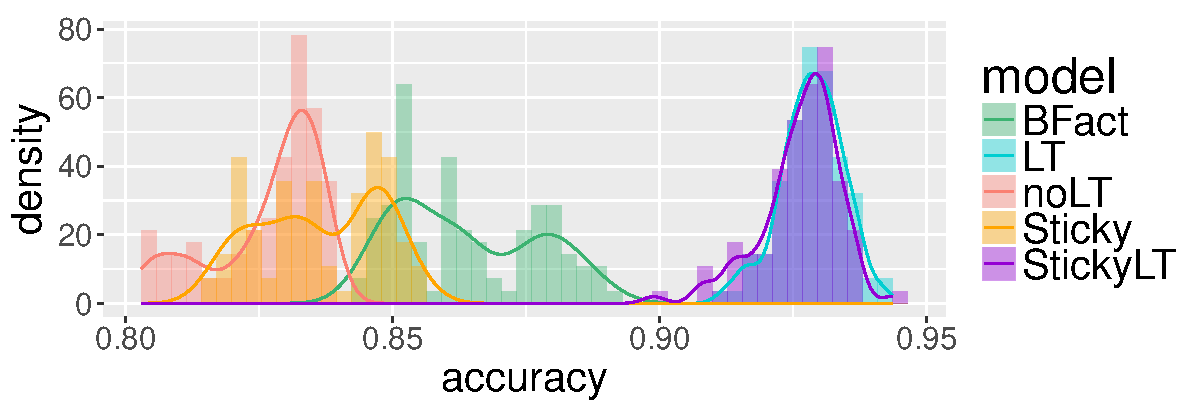
\includegraphics[width = \textwidth]{fig/cocktail/synth_s16_m12/hyper_gamma/h10.0_nocs_cp0/a0p01b0p01/accuracy_density.pdf}
\end{minipage}

\begin{minipage}{0.75\textwidth}
  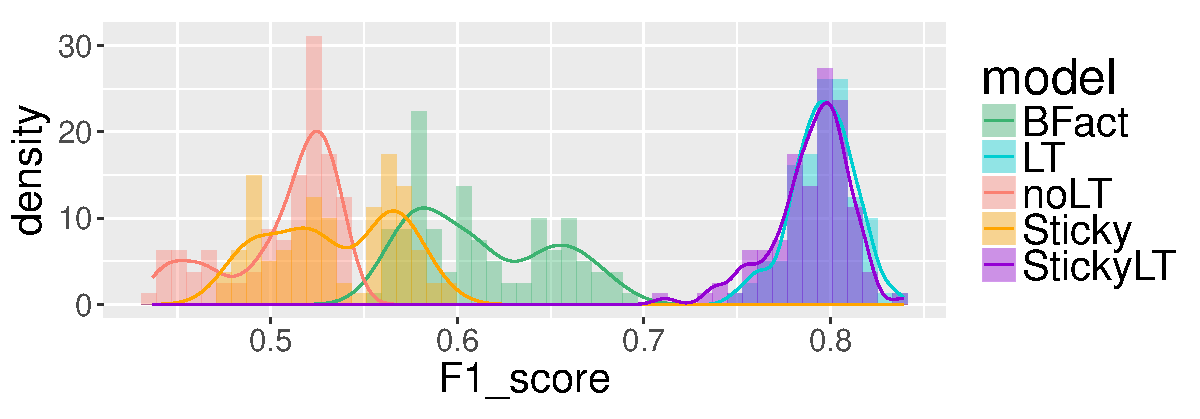
\includegraphics[width = \textwidth]{fig/cocktail/synth_s16_m12/hyper_gamma/h10.0_nocs_cp0/a0p01b0p01/F1_score_density.pdf}
\end{minipage}

\begin{minipage}{0.75\textwidth}
  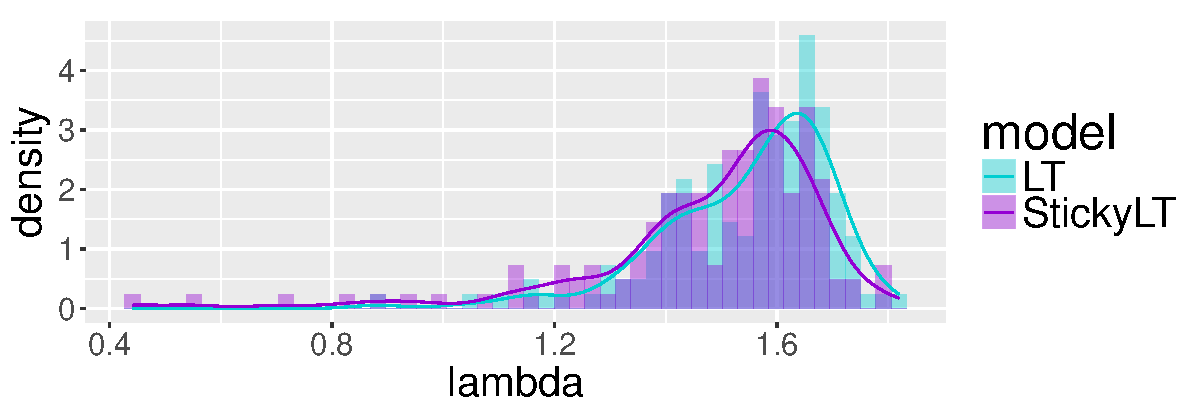
\includegraphics[width = \textwidth]{fig/cocktail/synth_s16_m12/hyper_gamma/h10.0_nocs_cp0/a0p01b0p01/lambda_density.pdf}
\end{minipage}

\begin{minipage}{0.75\textwidth}
  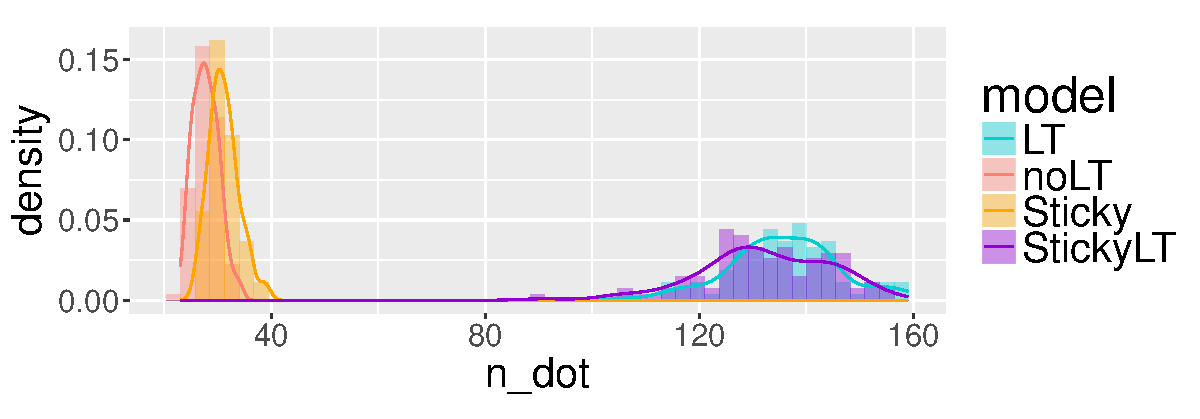
\includegraphics[width = \textwidth]{fig/cocktail/synth_s16_m12/hyper_gamma/h10.0_nocs_cp0/a0p01b0p01/n_dot_density.pdf}
\end{minipage}
\caption{Metrics for run 1: $\gamma \sim \Gamm{0.01}{0.01}$}
\end{figure}

\begin{figure}[tb]
% \vskip 0.1in
\begin{center}
  \centerline{\includegraphics[width = \textwidth, height = 0.2\textwidth]{fig/cocktail/synth_s16_m12/hyper_gamma/h10.0_nocs_cp0/a0p01b0p01/groundtruth.pdf}}
  \centerline{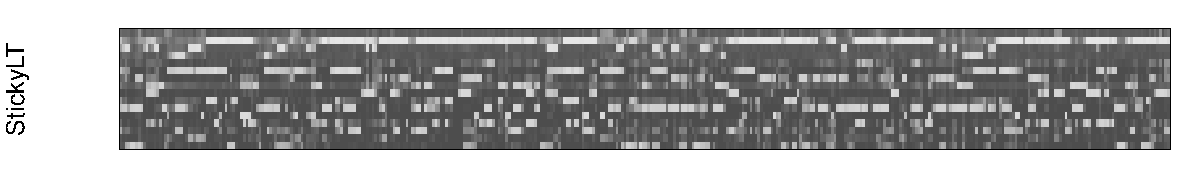
\includegraphics[width = \textwidth, height = 0.2\textwidth]{fig/cocktail/synth_s16_m12/hyper_gamma/h10.0_nocs_cp0/a0p01b0p01/StickyLT_hdp_hmm_w0_agamma0p01_bgamma0p01/binary_state.pdf}}
  \centerline{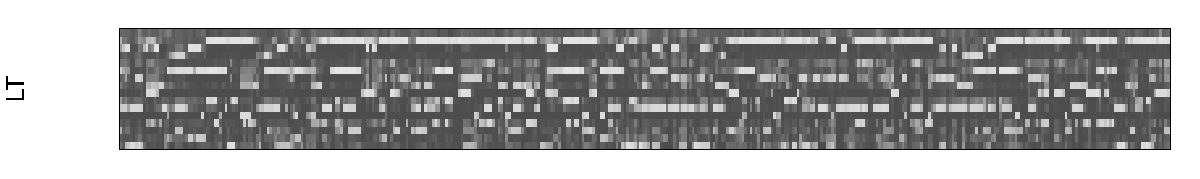
\includegraphics[width = \textwidth, height = 0.2\textwidth]{fig/cocktail/synth_s16_m12/hyper_gamma/h10.0_nocs_cp0/a0p01b0p01/LT_hdp_hmm_w0_agamma0p01_bgamma0p01/binary_state.pdf}}
  \centerline{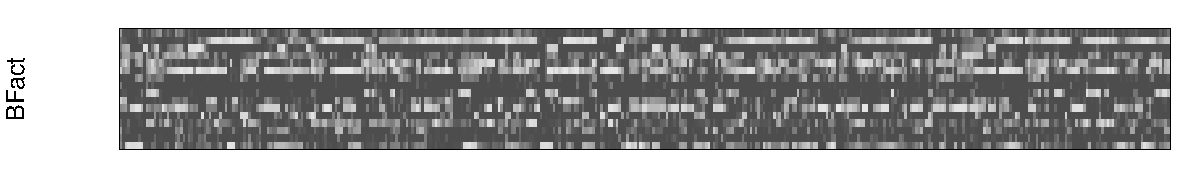
\includegraphics[width = \textwidth, height = 0.2\textwidth]{fig/cocktail/synth_s16_m12/hyper_gamma/h10.0_nocs_cp0/a0p01b0p01/BFact_hmm_w0_agamma0p01_bgamma0p01/binary_state.pdf}}
  \centerline{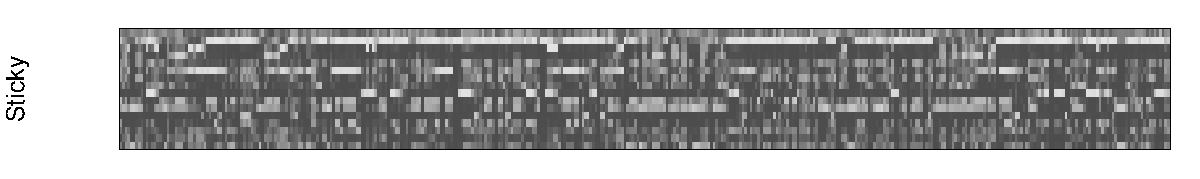
\includegraphics[width = \textwidth, height = 0.2\textwidth]{fig/cocktail/synth_s16_m12/hyper_gamma/h10.0_nocs_cp0/a0p01b0p01/Sticky_hdp_hmm_w0_agamma0p01_bgamma0p01/binary_state.pdf}}
  \centerline{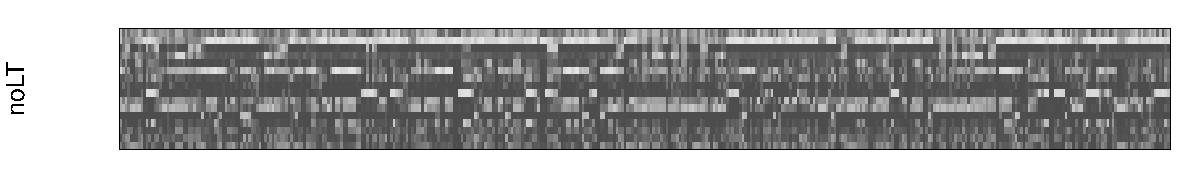
\includegraphics[width = \textwidth, height = 0.2\textwidth]{fig/cocktail/synth_s16_m12/hyper_gamma/h10.0_nocs_cp0/a0p01b0p01/noLT_hdp_hmm_w0_agamma0p01_bgamma0p01/binary_state.pdf}}
\caption{Binary speaker matrices for run 1: $\gamma \sim \Gamm{0.01}{0.01}$}
\end{center}
\end{figure}


\begin{figure}[tb]
  \centering
  \begin{minipage}{0.75\textwidth}
  \includegraphics[width = \textwidth]{fig/cocktail/synth_s16_m12/hyper_gamma/h10.0_nocs_cp0/a0p01b5/accuracy_density.pdf}
\end{minipage}

\begin{minipage}{0.75\textwidth}
  \includegraphics[width = \textwidth]{fig/cocktail/synth_s16_m12/hyper_gamma/h10.0_nocs_cp0/a0p01b5/F1_score_density.pdf}
\end{minipage}

\begin{minipage}{0.75\textwidth}
  \includegraphics[width = \textwidth]{fig/cocktail/synth_s16_m12/hyper_gamma/h10.0_nocs_cp0/a0p01b5/lambda_density.pdf}
\end{minipage}

\begin{minipage}{0.75\textwidth}
  \includegraphics[width = \textwidth]{fig/cocktail/synth_s16_m12/hyper_gamma/h10.0_nocs_cp0/a0p01b5/n_dot_density.pdf}
\end{minipage}
\caption{Metrics for run 2: $\gamma \sim \Gamm{0.01}{5}$}
\end{figure}

\begin{figure}[tb]
% \vskip 0.1in
\begin{center}
  \centerline{\includegraphics[width = \textwidth, height = 0.2\textwidth]{fig/cocktail/synth_s16_m12/hyper_gamma/h10.0_nocs_cp0/a0p01b5/groundtruth.pdf}}
  \centerline{\includegraphics[width = \textwidth, height = 0.2\textwidth]{fig/cocktail/synth_s16_m12/hyper_gamma/h10.0_nocs_cp0/a0p01b5/StickyLT_hdp_hmm_w0_agamma0p01_bgamma5/binary_state.pdf}}
  \centerline{\includegraphics[width = \textwidth, height = 0.2\textwidth]{fig/cocktail/synth_s16_m12/hyper_gamma/h10.0_nocs_cp0/a0p01b5/LT_hdp_hmm_w0_agamma0p01_bgamma5/binary_state.pdf}}
  \centerline{\includegraphics[width = \textwidth, height = 0.2\textwidth]{fig/cocktail/synth_s16_m12/hyper_gamma/h10.0_nocs_cp0/a0p01b5/BFact_hmm_w0_agamma0p01_bgamma5/binary_state.pdf}}
  \centerline{\includegraphics[width = \textwidth, height = 0.2\textwidth]{fig/cocktail/synth_s16_m12/hyper_gamma/h10.0_nocs_cp0/a0p01b5/Sticky_hdp_hmm_w0_agamma0p01_bgamma5/binary_state.pdf}}
  \centerline{\includegraphics[width = \textwidth, height = 0.2\textwidth]{fig/cocktail/synth_s16_m12/hyper_gamma/h10.0_nocs_cp0/a0p01b5/noLT_hdp_hmm_w0_agamma0p01_bgamma5/binary_state.pdf}}
\caption{Binary speaker matrices for run 2: $\gamma \sim \Gamm{0.01}{5}$}
\end{center}
\end{figure}

\begin{figure}[tb]
  \centering
  \begin{minipage}{0.75\textwidth}
  \includegraphics[width = \textwidth]{fig/cocktail/synth_s16_m12/hyper_gamma/h10.0_nocs_cp0/a5b0p01/accuracy_density.pdf}
\end{minipage}

\begin{minipage}{0.75\textwidth}
  \includegraphics[width = \textwidth]{fig/cocktail/synth_s16_m12/hyper_gamma/h10.0_nocs_cp0/a5b0p01/F1_score_density.pdf}
\end{minipage}

\begin{minipage}{0.75\textwidth}
  \includegraphics[width = \textwidth]{fig/cocktail/synth_s16_m12/hyper_gamma/h10.0_nocs_cp0/a5b0p01/lambda_density.pdf}
\end{minipage}

\begin{minipage}{0.75\textwidth}
  \includegraphics[width = \textwidth]{fig/cocktail/synth_s16_m12/hyper_gamma/h10.0_nocs_cp0/a5b0p01/n_dot_density.pdf}
\end{minipage}
\caption{Metrics for run 3: $\gamma \sim \Gamm{5}{0.01}$}
\end{figure}

\begin{figure}[tb]
% \vskip 0.1in
\begin{center}
  \centerline{\includegraphics[width = \textwidth, height = 0.2\textwidth]{fig/cocktail/synth_s16_m12/hyper_gamma/h10.0_nocs_cp0/a5b0p01/groundtruth.pdf}}
  \centerline{\includegraphics[width = \textwidth, height = 0.2\textwidth]{fig/cocktail/synth_s16_m12/hyper_gamma/h10.0_nocs_cp0/a5b0p01/StickyLT_hdp_hmm_w0_agamma5_bgamma0p01/binary_state.pdf}}
  \centerline{\includegraphics[width = \textwidth, height = 0.2\textwidth]{fig/cocktail/synth_s16_m12/hyper_gamma/h10.0_nocs_cp0/a5b0p01/LT_hdp_hmm_w0_agamma5_bgamma0p01/binary_state.pdf}}
  \centerline{\includegraphics[width = \textwidth, height = 0.2\textwidth]{fig/cocktail/synth_s16_m12/hyper_gamma/h10.0_nocs_cp0/a5b0p01/BFact_hmm_w0_agamma5_bgamma0p01/binary_state.pdf}}
  \centerline{\includegraphics[width = \textwidth, height = 0.2\textwidth]{fig/cocktail/synth_s16_m12/hyper_gamma/h10.0_nocs_cp0/a5b0p01/Sticky_hdp_hmm_w0_agamma5_bgamma0p01/binary_state.pdf}}
  \centerline{\includegraphics[width = \textwidth, height = 0.2\textwidth]{fig/cocktail/synth_s16_m12/hyper_gamma/h10.0_nocs_cp0/a5b0p01/noLT_hdp_hmm_w0_agamma5_bgamma0p01/binary_state.pdf}}
\caption{Binary speaker matrices for run 3: $\gamma \sim \Gamm{5}{0.01}$}
\end{center}
\end{figure}

\begin{figure}[tb]
  \centering
  \begin{minipage}{0.75\textwidth}
  \includegraphics[width = \textwidth]{fig/cocktail/synth_s16_m12/hyper_gamma/h10.0_nocs_cp0/a5b5/accuracy_density.pdf}
\end{minipage}

\begin{minipage}{0.75\textwidth}
  \includegraphics[width = \textwidth]{fig/cocktail/synth_s16_m12/hyper_gamma/h10.0_nocs_cp0/a5b5/F1_score_density.pdf}
\end{minipage}

\begin{minipage}{0.75\textwidth}
  \includegraphics[width = \textwidth]{fig/cocktail/synth_s16_m12/hyper_gamma/h10.0_nocs_cp0/a5b5/lambda_density.pdf}
\end{minipage}

\begin{minipage}{0.75\textwidth}
  \includegraphics[width = \textwidth]{fig/cocktail/synth_s16_m12/hyper_gamma/h10.0_nocs_cp0/a5b5/n_dot_density.pdf}
\end{minipage}
\caption{Metrics for run 4: $\gamma \sim \Gamm{5}{5}$}
\end{figure}

\begin{figure}[tb]
% \vskip 0.1in
\begin{center}
  \centerline{\includegraphics[width = \textwidth, height = 0.2\textwidth]{fig/cocktail/synth_s16_m12/hyper_gamma/h10.0_nocs_cp0/a5b5/groundtruth.pdf}}
  \centerline{\includegraphics[width = \textwidth, height = 0.2\textwidth]{fig/cocktail/synth_s16_m12/hyper_gamma/h10.0_nocs_cp0/a5b5/StickyLT_hdp_hmm_w0_agamma5_bgamma5/binary_state.pdf}}
  \centerline{\includegraphics[width = \textwidth, height = 0.2\textwidth]{fig/cocktail/synth_s16_m12/hyper_gamma/h10.0_nocs_cp0/a5b5/LT_hdp_hmm_w0_agamma5_bgamma5/binary_state.pdf}}
  \centerline{\includegraphics[width = \textwidth, height = 0.2\textwidth]{fig/cocktail/synth_s16_m12/hyper_gamma/h10.0_nocs_cp0/a5b5/BFact_hmm_w0_agamma5_bgamma5/binary_state.pdf}}
  \centerline{\includegraphics[width = \textwidth, height = 0.2\textwidth]{fig/cocktail/synth_s16_m12/hyper_gamma/h10.0_nocs_cp0/a5b5/Sticky_hdp_hmm_w0_agamma5_bgamma5/binary_state.pdf}}
  \centerline{\includegraphics[width = \textwidth, height = 0.2\textwidth]{fig/cocktail/synth_s16_m12/hyper_gamma/h10.0_nocs_cp0/a5b5/noLT_hdp_hmm_w0_agamma5_bgamma5/binary_state.pdf}}
\caption{Binary speaker matrices for run 4: $\gamma \sim \Gamm{5}{5}$}
\end{center}
\end{figure}


\begin{figure}[tb]
  \centering
  \begin{minipage}{0.75\textwidth}
  \includegraphics[width = \textwidth]{fig/cocktail/synth_s16_m12/hyper_alpha/h10.0_nocs_cp0/a0p01b0p01/accuracy_density.pdf}
\end{minipage}

\begin{minipage}{0.75\textwidth}
  \includegraphics[width = \textwidth]{fig/cocktail/synth_s16_m12/hyper_alpha/h10.0_nocs_cp0/a0p01b0p01/F1_score_density.pdf}
\end{minipage}

\begin{minipage}{0.75\textwidth}
  \includegraphics[width = \textwidth]{fig/cocktail/synth_s16_m12/hyper_alpha/h10.0_nocs_cp0/a0p01b0p01/lambda_density.pdf}
\end{minipage}

\begin{minipage}{0.75\textwidth}
  \includegraphics[width = \textwidth]{fig/cocktail/synth_s16_m12/hyper_alpha/h10.0_nocs_cp0/a0p01b0p01/n_dot_density.pdf}
\end{minipage}
\caption{Metrics for run 5: $\alpha \sim \Gamm{0.01}{0.01}$}
\end{figure}

\begin{figure}[tb]
% \vskip 0.1in
\begin{center}
  \centerline{\includegraphics[width = \textwidth, height = 0.2\textwidth]{fig/cocktail/synth_s16_m12/hyper_alpha/h10.0_nocs_cp0/a0p01b0p01/groundtruth.pdf}}
  \centerline{\includegraphics[width = \textwidth, height = 0.2\textwidth]{fig/cocktail/synth_s16_m12/hyper_alpha/h10.0_nocs_cp0/a0p01b0p01/StickyLT_hdp_hmm_w0_aalpha0p01_balpha0p01/binary_state.pdf}}
  \centerline{\includegraphics[width = \textwidth, height = 0.2\textwidth]{fig/cocktail/synth_s16_m12/hyper_alpha/h10.0_nocs_cp0/a0p01b0p01/LT_hdp_hmm_w0_aalpha0p01_balpha0p01/binary_state.pdf}}
  \centerline{\includegraphics[width = \textwidth, height = 0.2\textwidth]{fig/cocktail/synth_s16_m12/hyper_alpha/h10.0_nocs_cp0/a0p01b0p01/BFact_hmm_w0_aalpha0p01_balpha0p01/binary_state.pdf}}
  \centerline{\includegraphics[width = \textwidth, height = 0.2\textwidth]{fig/cocktail/synth_s16_m12/hyper_alpha/h10.0_nocs_cp0/a0p01b0p01/Sticky_hdp_hmm_w0_aalpha0p01_balpha0p01/binary_state.pdf}}
  \centerline{\includegraphics[width = \textwidth, height = 0.2\textwidth]{fig/cocktail/synth_s16_m12/hyper_alpha/h10.0_nocs_cp0/a0p01b0p01/noLT_hdp_hmm_w0_aalpha0p01_balpha0p01/binary_state.pdf}}
\caption{Binary speaker matrices for run 5: $\alpha \sim \Gamm{0.01}{0.01}$}
\end{center}
\end{figure}


\begin{figure}[tb]
  \centering
  \begin{minipage}{0.75\textwidth}
  \includegraphics[width = \textwidth]{fig/cocktail/synth_s16_m12/hyper_alpha/h10.0_nocs_cp0/a0p01b5/accuracy_density.pdf}
\end{minipage}

\begin{minipage}{0.75\textwidth}
  \includegraphics[width = \textwidth]{fig/cocktail/synth_s16_m12/hyper_alpha/h10.0_nocs_cp0/a0p01b5/F1_score_density.pdf}
\end{minipage}

\begin{minipage}{0.75\textwidth}
  \includegraphics[width = \textwidth]{fig/cocktail/synth_s16_m12/hyper_alpha/h10.0_nocs_cp0/a0p01b5/lambda_density.pdf}
\end{minipage}

\begin{minipage}{0.75\textwidth}
  \includegraphics[width = \textwidth]{fig/cocktail/synth_s16_m12/hyper_alpha/h10.0_nocs_cp0/a0p01b5/n_dot_density.pdf}
\end{minipage}
\caption{Metrics for run 6: $\alpha \sim \Gamm{0.01}{5}$}
\end{figure}

\begin{figure}[tb]
% \vskip 0.1in
\begin{center}
  \centerline{\includegraphics[width = \textwidth, height = 0.2\textwidth]{fig/cocktail/synth_s16_m12/hyper_alpha/h10.0_nocs_cp0/a0p01b5/groundtruth.pdf}}
  \centerline{\includegraphics[width = \textwidth, height = 0.2\textwidth]{fig/cocktail/synth_s16_m12/hyper_alpha/h10.0_nocs_cp0/a0p01b5/StickyLT_hdp_hmm_w0_aalpha0p01_balpha5/binary_state.pdf}}
  \centerline{\includegraphics[width = \textwidth, height = 0.2\textwidth]{fig/cocktail/synth_s16_m12/hyper_alpha/h10.0_nocs_cp0/a0p01b5/LT_hdp_hmm_w0_aalpha0p01_balpha5/binary_state.pdf}}
  \centerline{\includegraphics[width = \textwidth, height = 0.2\textwidth]{fig/cocktail/synth_s16_m12/hyper_alpha/h10.0_nocs_cp0/a0p01b5/BFact_hmm_w0_aalpha0p01_balpha5/binary_state.pdf}}
  \centerline{\includegraphics[width = \textwidth, height = 0.2\textwidth]{fig/cocktail/synth_s16_m12/hyper_alpha/h10.0_nocs_cp0/a0p01b5/Sticky_hdp_hmm_w0_aalpha0p01_balpha5/binary_state.pdf}}
  \centerline{\includegraphics[width = \textwidth, height = 0.2\textwidth]{fig/cocktail/synth_s16_m12/hyper_alpha/h10.0_nocs_cp0/a0p01b5/noLT_hdp_hmm_w0_aalpha0p01_balpha5/binary_state.pdf}}
\caption{Binary speaker matrices for run 6: $\alpha \sim \Gamm{0.01}{5}$}
\end{center}
\end{figure}

\begin{figure}[tb]
  \centering
  \begin{minipage}{0.75\textwidth}
  \includegraphics[width = \textwidth]{fig/cocktail/synth_s16_m12/hyper_alpha/h10.0_nocs_cp0/a5b0p01/accuracy_density.pdf}
\end{minipage}

\begin{minipage}{0.75\textwidth}
  \includegraphics[width = \textwidth]{fig/cocktail/synth_s16_m12/hyper_alpha/h10.0_nocs_cp0/a5b0p01/F1_score_density.pdf}
\end{minipage}

\begin{minipage}{0.75\textwidth}
  \includegraphics[width = \textwidth]{fig/cocktail/synth_s16_m12/hyper_alpha/h10.0_nocs_cp0/a5b0p01/lambda_density.pdf}
\end{minipage}

\begin{minipage}{0.75\textwidth}
  \includegraphics[width = \textwidth]{fig/cocktail/synth_s16_m12/hyper_alpha/h10.0_nocs_cp0/a5b0p01/n_dot_density.pdf}
\end{minipage}
\caption{Metrics for run 7: $\alpha \sim \Gamm{5}{0.01}$}
\end{figure}

\begin{figure}[tb]
% \vskip 0.1in
\begin{center}
  \centerline{\includegraphics[width = \textwidth, height = 0.2\textwidth]{fig/cocktail/synth_s16_m12/hyper_alpha/h10.0_nocs_cp0/a5b0p01/groundtruth.pdf}}
  \centerline{\includegraphics[width = \textwidth, height = 0.2\textwidth]{fig/cocktail/synth_s16_m12/hyper_alpha/h10.0_nocs_cp0/a5b0p01/StickyLT_hdp_hmm_w0_aalpha5_balpha0p01/binary_state.pdf}}
  \centerline{\includegraphics[width = \textwidth, height = 0.2\textwidth]{fig/cocktail/synth_s16_m12/hyper_alpha/h10.0_nocs_cp0/a5b0p01/LT_hdp_hmm_w0_aalpha5_balpha0p01/binary_state.pdf}}
  \centerline{\includegraphics[width = \textwidth, height = 0.2\textwidth]{fig/cocktail/synth_s16_m12/hyper_alpha/h10.0_nocs_cp0/a5b0p01/BFact_hmm_w0_aalpha5_balpha0p01/binary_state.pdf}}
  \centerline{\includegraphics[width = \textwidth, height = 0.2\textwidth]{fig/cocktail/synth_s16_m12/hyper_alpha/h10.0_nocs_cp0/a5b0p01/Sticky_hdp_hmm_w0_aalpha5_balpha0p01/binary_state.pdf}}
  \centerline{\includegraphics[width = \textwidth, height = 0.2\textwidth]{fig/cocktail/synth_s16_m12/hyper_alpha/h10.0_nocs_cp0/a5b0p01/noLT_hdp_hmm_w0_aalpha5_balpha0p01/binary_state.pdf}}
\caption{Binary speaker matrices for run 7: $\alpha \sim \Gamm{5}{0.01}$}
\end{center}
\end{figure}

\begin{figure}[tb]
  \centering
  \begin{minipage}{0.75\textwidth}
  \includegraphics[width = \textwidth]{fig/cocktail/synth_s16_m12/hyper_alpha/h10.0_nocs_cp0/a5b5/accuracy_density.pdf}
\end{minipage}

\begin{minipage}{0.75\textwidth}
  \includegraphics[width = \textwidth]{fig/cocktail/synth_s16_m12/hyper_alpha/h10.0_nocs_cp0/a5b5/F1_score_density.pdf}
\end{minipage}

\begin{minipage}{0.75\textwidth}
  \includegraphics[width = \textwidth]{fig/cocktail/synth_s16_m12/hyper_alpha/h10.0_nocs_cp0/a5b5/lambda_density.pdf}
\end{minipage}

\begin{minipage}{0.75\textwidth}
  \includegraphics[width = \textwidth]{fig/cocktail/synth_s16_m12/hyper_alpha/h10.0_nocs_cp0/a5b5/n_dot_density.pdf}
\end{minipage}
\caption{Metrics for run 8: $\alpha \sim \Gamm{5}{5}$}
\end{figure}

\begin{figure}[tb]
% \vskip 0.1in
\begin{center}
  \centerline{\includegraphics[width = \textwidth, height = 0.2\textwidth]{fig/cocktail/synth_s16_m12/hyper_alpha/h10.0_nocs_cp0/a5b5/groundtruth.pdf}}
  \centerline{\includegraphics[width = \textwidth, height = 0.2\textwidth]{fig/cocktail/synth_s16_m12/hyper_alpha/h10.0_nocs_cp0/a5b5/StickyLT_hdp_hmm_w0_aalpha5_balpha5/binary_state.pdf}}
  \centerline{\includegraphics[width = \textwidth, height = 0.2\textwidth]{fig/cocktail/synth_s16_m12/hyper_alpha/h10.0_nocs_cp0/a5b5/LT_hdp_hmm_w0_aalpha5_balpha5/binary_state.pdf}}
  \centerline{\includegraphics[width = \textwidth, height = 0.2\textwidth]{fig/cocktail/synth_s16_m12/hyper_alpha/h10.0_nocs_cp0/a5b5/BFact_hmm_w0_aalpha5_balpha5/binary_state.pdf}}
  \centerline{\includegraphics[width = \textwidth, height = 0.2\textwidth]{fig/cocktail/synth_s16_m12/hyper_alpha/h10.0_nocs_cp0/a5b5/Sticky_hdp_hmm_w0_aalpha5_balpha5/binary_state.pdf}}
  \centerline{\includegraphics[width = \textwidth, height = 0.2\textwidth]{fig/cocktail/synth_s16_m12/hyper_alpha/h10.0_nocs_cp0/a5b5/noLT_hdp_hmm_w0_aalpha5_balpha5/binary_state.pdf}}
\caption{Binary speaker matrices for run 8: $\alpha \sim \Gamm{5}{5}$}
\end{center}
\end{figure}


\begin{figure}[tb]
  \centering
  \begin{minipage}{0.75\textwidth}
  \includegraphics[width = \textwidth]{fig/cocktail/synth_s16_m12/hyper_h/h10.0_nocs_cp0/a0p01b0p01/accuracy_density.pdf}
\end{minipage}

\begin{minipage}{0.75\textwidth}
  \includegraphics[width = \textwidth]{fig/cocktail/synth_s16_m12/hyper_h/h10.0_nocs_cp0/a0p01b0p01/F1_score_density.pdf}
\end{minipage}

\begin{minipage}{0.75\textwidth}
  \includegraphics[width = \textwidth]{fig/cocktail/synth_s16_m12/hyper_h/h10.0_nocs_cp0/a0p01b0p01/lambda_density.pdf}
\end{minipage}

\begin{minipage}{0.75\textwidth}
  \includegraphics[width = \textwidth]{fig/cocktail/synth_s16_m12/hyper_h/h10.0_nocs_cp0/a0p01b0p01/n_dot_density.pdf}
\end{minipage}
\caption{Metrics for run 9: $h \sim \Gamm{0.01}{0.01}$}
\end{figure}

\begin{figure}[tb]
% \vskip 0.1in
\begin{center}
  \centerline{\includegraphics[width = \textwidth, height = 0.2\textwidth]{fig/cocktail/synth_s16_m12/hyper_h/h10.0_nocs_cp0/a0p01b0p01/groundtruth.pdf}}
  \centerline{\includegraphics[width = \textwidth, height = 0.2\textwidth]{fig/cocktail/synth_s16_m12/hyper_h/h10.0_nocs_cp0/a0p01b0p01/StickyLT_hdp_hmm_w0_ah0p01_bh0p01/binary_state.pdf}}
  \centerline{\includegraphics[width = \textwidth, height = 0.2\textwidth]{fig/cocktail/synth_s16_m12/hyper_h/h10.0_nocs_cp0/a0p01b0p01/LT_hdp_hmm_w0_ah0p01_bh0p01/binary_state.pdf}}
  \centerline{\includegraphics[width = \textwidth, height = 0.2\textwidth]{fig/cocktail/synth_s16_m12/hyper_h/h10.0_nocs_cp0/a0p01b0p01/BFact_hmm_w0_ah0p01_bh0p01/binary_state.pdf}}
  \centerline{\includegraphics[width = \textwidth, height = 0.2\textwidth]{fig/cocktail/synth_s16_m12/hyper_h/h10.0_nocs_cp0/a0p01b0p01/Sticky_hdp_hmm_w0_ah0p01_bh0p01/binary_state.pdf}}
  \centerline{\includegraphics[width = \textwidth, height = 0.2\textwidth]{fig/cocktail/synth_s16_m12/hyper_h/h10.0_nocs_cp0/a0p01b0p01/noLT_hdp_hmm_w0_ah0p01_bh0p01/binary_state.pdf}}
\caption{Binary speaker matrices for run 9: $h \sim \Gamm{0.01}{0.01}$}
\end{center}
\end{figure}


\begin{figure}[tb]
  \centering
  \begin{minipage}{0.75\textwidth}
  \includegraphics[width = \textwidth]{fig/cocktail/synth_s16_m12/hyper_h/h10.0_nocs_cp0/a0p01b5/accuracy_density.pdf}
\end{minipage}

\begin{minipage}{0.75\textwidth}
  \includegraphics[width = \textwidth]{fig/cocktail/synth_s16_m12/hyper_h/h10.0_nocs_cp0/a0p01b5/F1_score_density.pdf}
\end{minipage}

\begin{minipage}{0.75\textwidth}
  \includegraphics[width = \textwidth]{fig/cocktail/synth_s16_m12/hyper_h/h10.0_nocs_cp0/a0p01b5/lambda_density.pdf}
\end{minipage}

\begin{minipage}{0.75\textwidth}
  \includegraphics[width = \textwidth]{fig/cocktail/synth_s16_m12/hyper_h/h10.0_nocs_cp0/a0p01b5/n_dot_density.pdf}
\end{minipage}
\caption{Metrics for run 10: $h \sim \Gamm{0.01}{5}$}
\end{figure}

\begin{figure}[tb]
% \vskip 0.1in
\begin{center}
  \centerline{\includegraphics[width = \textwidth, height = 0.2\textwidth]{fig/cocktail/synth_s16_m12/hyper_h/h10.0_nocs_cp0/a0p01b5/groundtruth.pdf}}
  \centerline{\includegraphics[width = \textwidth, height = 0.2\textwidth]{fig/cocktail/synth_s16_m12/hyper_h/h10.0_nocs_cp0/a0p01b5/StickyLT_hdp_hmm_w0_ah0p01_bh5/binary_state.pdf}}
  \centerline{\includegraphics[width = \textwidth, height = 0.2\textwidth]{fig/cocktail/synth_s16_m12/hyper_h/h10.0_nocs_cp0/a0p01b5/LT_hdp_hmm_w0_ah0p01_bh5/binary_state.pdf}}
  \centerline{\includegraphics[width = \textwidth, height = 0.2\textwidth]{fig/cocktail/synth_s16_m12/hyper_h/h10.0_nocs_cp0/a0p01b5/BFact_hmm_w0_ah0p01_bh5/binary_state.pdf}}
  \centerline{\includegraphics[width = \textwidth, height = 0.2\textwidth]{fig/cocktail/synth_s16_m12/hyper_h/h10.0_nocs_cp0/a0p01b5/Sticky_hdp_hmm_w0_ah0p01_bh5/binary_state.pdf}}
  \centerline{\includegraphics[width = \textwidth, height = 0.2\textwidth]{fig/cocktail/synth_s16_m12/hyper_h/h10.0_nocs_cp0/a0p01b5/noLT_hdp_hmm_w0_ah0p01_bh5/binary_state.pdf}}
\caption{Binary speaker matrices for run 10: $h \sim \Gamm{0.01}{5}$}
\end{center}
\end{figure}

\begin{figure}[tb]
  \centering
  \begin{minipage}{0.75\textwidth}
  \includegraphics[width = \textwidth]{fig/cocktail/synth_s16_m12/hyper_h/h10.0_nocs_cp0/a5b0p01/accuracy_density.pdf}
\end{minipage}

\begin{minipage}{0.75\textwidth}
  \includegraphics[width = \textwidth]{fig/cocktail/synth_s16_m12/hyper_h/h10.0_nocs_cp0/a5b0p01/F1_score_density.pdf}
\end{minipage}

\begin{minipage}{0.75\textwidth}
  \includegraphics[width = \textwidth]{fig/cocktail/synth_s16_m12/hyper_h/h10.0_nocs_cp0/a5b0p01/lambda_density.pdf}
\end{minipage}

\begin{minipage}{0.75\textwidth}
  \includegraphics[width = \textwidth]{fig/cocktail/synth_s16_m12/hyper_h/h10.0_nocs_cp0/a5b0p01/n_dot_density.pdf}
\end{minipage}
\caption{Metrics for run 11: $h \sim \Gamm{5}{0.01}$}
\end{figure}

\begin{figure}[tb]
% \vskip 0.1in
\begin{center}
  \centerline{\includegraphics[width = \textwidth, height = 0.2\textwidth]{fig/cocktail/synth_s16_m12/hyper_h/h10.0_nocs_cp0/a5b0p01/groundtruth.pdf}}
  \centerline{\includegraphics[width = \textwidth, height = 0.2\textwidth]{fig/cocktail/synth_s16_m12/hyper_h/h10.0_nocs_cp0/a5b0p01/StickyLT_hdp_hmm_w0_ah5_bh0p01/binary_state.pdf}}
  \centerline{\includegraphics[width = \textwidth, height = 0.2\textwidth]{fig/cocktail/synth_s16_m12/hyper_h/h10.0_nocs_cp0/a5b0p01/LT_hdp_hmm_w0_ah5_bh0p01/binary_state.pdf}}
  \centerline{\includegraphics[width = \textwidth, height = 0.2\textwidth]{fig/cocktail/synth_s16_m12/hyper_h/h10.0_nocs_cp0/a5b0p01/BFact_hmm_w0_ah5_bh0p01/binary_state.pdf}}
  \centerline{\includegraphics[width = \textwidth, height = 0.2\textwidth]{fig/cocktail/synth_s16_m12/hyper_h/h10.0_nocs_cp0/a5b0p01/Sticky_hdp_hmm_w0_ah5_bh0p01/binary_state.pdf}}
  \centerline{\includegraphics[width = \textwidth, height = 0.2\textwidth]{fig/cocktail/synth_s16_m12/hyper_h/h10.0_nocs_cp0/a5b0p01/noLT_hdp_hmm_w0_ah5_bh0p01/binary_state.pdf}}
\caption{Binary speaker matrices for run 11: $h \sim \Gamm{5}{0.01}$}
\end{center}
\end{figure}

\begin{figure}[tb]
  \centering
  \begin{minipage}{0.75\textwidth}
  \includegraphics[width = \textwidth]{fig/cocktail/synth_s16_m12/hyper_h/h10.0_nocs_cp0/a5b5/accuracy_density.pdf}
\end{minipage}

\begin{minipage}{0.75\textwidth}
  \includegraphics[width = \textwidth]{fig/cocktail/synth_s16_m12/hyper_h/h10.0_nocs_cp0/a5b5/F1_score_density.pdf}
\end{minipage}

\begin{minipage}{0.75\textwidth}
  \includegraphics[width = \textwidth]{fig/cocktail/synth_s16_m12/hyper_h/h10.0_nocs_cp0/a5b5/lambda_density.pdf}
\end{minipage}

\begin{minipage}{0.75\textwidth}
  \includegraphics[width = \textwidth]{fig/cocktail/synth_s16_m12/hyper_h/h10.0_nocs_cp0/a5b5/n_dot_density.pdf}
\end{minipage}
\caption{Metrics for run 12: $h \sim \Gamm{5}{5}$}
\end{figure}

\begin{figure}[tb]
% \vskip 0.1in
\begin{center}
  \centerline{\includegraphics[width = \textwidth, height = 0.2\textwidth]{fig/cocktail/synth_s16_m12/hyper_h/h10.0_nocs_cp0/a5b5/groundtruth.pdf}}
  \centerline{\includegraphics[width = \textwidth, height = 0.2\textwidth]{fig/cocktail/synth_s16_m12/hyper_h/h10.0_nocs_cp0/a5b5/StickyLT_hdp_hmm_w0_ah5_bh5/binary_state.pdf}}
  \centerline{\includegraphics[width = \textwidth, height = 0.2\textwidth]{fig/cocktail/synth_s16_m12/hyper_h/h10.0_nocs_cp0/a5b5/LT_hdp_hmm_w0_ah5_bh5/binary_state.pdf}}
  \centerline{\includegraphics[width = \textwidth, height = 0.2\textwidth]{fig/cocktail/synth_s16_m12/hyper_h/h10.0_nocs_cp0/a5b5/BFact_hmm_w0_ah5_bh5/binary_state.pdf}}
  \centerline{\includegraphics[width = \textwidth, height = 0.2\textwidth]{fig/cocktail/synth_s16_m12/hyper_h/h10.0_nocs_cp0/a5b5/Sticky_hdp_hmm_w0_ah5_bh5/binary_state.pdf}}
  \centerline{\includegraphics[width = \textwidth, height = 0.2\textwidth]{fig/cocktail/synth_s16_m12/hyper_h/h10.0_nocs_cp0/a5b5/noLT_hdp_hmm_w0_ah5_bh5/binary_state.pdf}}
\caption{Binary speaker matrices for run 12: $h \sim \Gamm{5}{5}$}
\end{center}
\end{figure}

\section{Bach Chorale Data}

The models used in the music experiments in Chapter \ref{chapter:music}
employ separate emission and similarity spaces, and hence, conditioned
on the state sequence, the observations do not inform the locations,
$\ell_j$.  As a result there is no extrinsic information about the
scale of the similarity kernel, since performing a rescaling of the
locations $\ell_j$ together with an inverse scaling of the kernel
parameter $\lambda$ results in an equivalent likelihood.  Therefore,
rather than letting $\lambda$ be inferred as it is in the cocktail
party experiments, its value was fixed, whereas the locations are
given a multivariate $\Norm{0}{\mathbf{I}}$ prior (in all experiments
reported here the dimension of the similarity space is $2$)
and are sampled using Hamiltonian Monte Carlo.

Although sampling state locations in principle allows similarities to be learned,
the choice of scale parameter $\lambda$ relative to the prior on state
locations is consequential in practice.  In
Figs. \ref{fig:bach-hyperparameter-lambda0p01}-\ref{fig:bach-hyperparameter-lambda5p0},
training and test set log likelihoods are shown on the Bach chorale data for four models ---
HDP-HMM, Sticky HDP-HMM, HDP-HMM-LT, and Sticky HDP-HMM-LT --- with
$\lambda$ values of 0.01, 1.0 and 5.0, respectively.  In
Fig. \ref{fig:bach-hyperparameter-all-lambdas}, the effect of
$\lambda$ on the log likelihood is shown for a spectrum of models
ranging from the original HDP-HMM ($\lambda = 0$) to an HDP-HMM-LT
with $\lambda = 10$.

The pattern reported in Chapter \ref{chapter:music} can be seen
clearly in these results: with very small $\lambda$ (0.01), the LT
models are nearly identical to the non-LT models.  As $\lambda$
increases up to 5, the gap increases, with the LT models achieving
lower training log likelihoods and higher test log likelihoods,
reflecting the tendency of the non-LT models' less restrictive prior on transition
matrices to overfit by employing as many states as possible.  When
$\lambda$ gets as large as 10, however, performance degrades, with
both training and test log likelihoods decreasing.  This likely
reflects a too-strong bias toward self-transitions, resulting in the
use of too few states and underfitting the data.

\begin{figure}[tb]
% \vskip 0.1in
\begin{center}
  \centerline{\includegraphics[width = 0.75\columnwidth]{fig/music/bach/lambda0p01/train_log_likelihood_density.pdf}}
  \centerline{\includegraphics[width = 0.75\columnwidth]{fig/music/bach/lambda0p01/test_log_likelihood_density.pdf}}
  \centerline{\includegraphics[width = 0.75\columnwidth]{fig/music/bach/lambda0p01/n_dot_density.pdf}}
  % \centerline{\includegraphics[width = \columnwidth]{fig/bach/alpha.pdf}}
\caption{Top and Middle: Training set and test set log marginal likelihoods for Bach
  chorale data on the four HDP-based models: HDP-HMM-LT, HDP-HMM,
  Sticky HMM, and Sticky HDP-HMM-LT, where the two LT models set
  $\lambda = 0.01$.  Bottom: Number of latent states
  occupied in the training set by each model. \label{fig:bach-hyperparameter-lambda0p01}
}
\end{center}
% \vskip 0.1in
\end{figure}

\begin{figure}[tb]
% \vskip 0.1in
\begin{center}
  \centerline{\includegraphics[width = 0.75\columnwidth]{fig/music/bach/lambda1/train_log_likelihood_density.pdf}}
  \centerline{\includegraphics[width = 0.75\columnwidth]{fig/music/bach/lambda1/test_log_likelihood_density.pdf}}
  \centerline{\includegraphics[width = 0.75\columnwidth]{fig/music/bach/lambda1/n_dot_density.pdf}}
  % \centerline{\includegraphics[width = \columnwidth]{fig/bach/alpha.pdf}}
\caption{Top and Middle: Training set and test set log marginal likelihoods for Bach
  chorale data on the four HDP-based models: HDP-HMM-LT, HDP-HMM,
  Sticky HMM, and Sticky HDP-HMM-LT, where the two LT models set
  $\lambda = 1.0$.  Bottom: Number of latent states
  occupied in the training set by each model. \label{fig:bach-hyperparameter-lambda1p0}
}
\end{center}
% \vskip 0.1in
\end{figure}

\begin{figure}[tb]
% \vskip 0.1in
\begin{center}
  \centerline{\includegraphics[width = 0.75\columnwidth]{fig/music/bach/lambda5/train_log_likelihood_density.pdf}}
  \centerline{\includegraphics[width = 0.75\columnwidth]{fig/music/bach/lambda5/test_log_likelihood_density.pdf}}
  \centerline{\includegraphics[width = 0.75\columnwidth]{fig/music/bach/lambda5/n_dot_density.pdf}}
  % \centerline{\includegraphics[width = \columnwidth]{fig/bach/alpha.pdf}}
\caption{Top and Middle: Training set and test set log marginal likelihoods for Bach
  chorale data on the four HDP-based models: HDP-HMM-LT, HDP-HMM,
  Sticky HMM, and Sticky HDP-HMM-LT, where the two LT models set
  $\lambda = 1.0$.  Bottom: Number of latent states
  occupied in the training set by each model. \label{fig:bach-hyperparameter-lambda5p0}
}
\end{center}
% \vskip 0.1in
\end{figure}

\begin{figure}[tb]
% \vskip 0.1in
\begin{center}
  \centerline{\includegraphics[width = 0.75\columnwidth]{fig/music/bach/varying_lambda_eps0005/train_log_likelihood_density.pdf}}
  \centerline{\includegraphics[width = 0.75\columnwidth]{fig/music/bach/varying_lambda_eps0005/test_log_likelihood_density.pdf}}
  \centerline{\includegraphics[width = 0.75\columnwidth]{fig/music/bach/varying_lambda_eps0005/n_dot_density.pdf}}
  % \centerline{\includegraphics[width = \columnwidth]{fig/bach/alpha.pdf}}
\caption{Top and Middle: Training set and test set log marginal likelihoods for Bach
  chorale data on the four HDP-based models: HDP-HMM-LT, HDP-HMM,
  Sticky HMM, and Sticky HDP-HMM-LT, where the two LT models set
  $\lambda = 1.0$.  Bottom: Number of latent states
  occupied in the training set by each model. \label{fig:bach-hyperparameter-all-lambdas}
}
\end{center}
% \vskip 0.1in
\end{figure}


\bibliographystyle{apalike}
\bibliography{../bib/supplement}
\end{document}  
